\documentclass[prd,aps,10pt,nofootinbib,twocolumn,superscriptaddress,preprintnumbers,balancelastpage,longbibliography]{revtex4-1}

\usepackage{amsmath,amssymb}	
\usepackage{mathtools}
\usepackage{fontawesome}
\usepackage[dvipsnames]{xcolor}
\usepackage{hyperref}
\usepackage{xspace}
\usepackage{fancyhdr}
\usepackage{braket}
\usepackage{graphicx}
\usepackage{siunitx}
\usepackage{blindtext}
\usepackage{nicefrac}
\usepackage{lipsum}
\usepackage{bbold}
\usepackage{tabularx}
\usepackage{multirow}
% \usepackage{booktabs}
\usepackage{dcolumn}
\usepackage{makecell}

\usepackage{afterpage}
% \newcolumntype{L}[1]{>{\raggedright\let\newline\\\arraybackslash\hspace{0pt}}m{#1}}
% \newcolumntype{C}[1]{>{\centering\let\newline\\\arraybackslash\hspace{0pt}}m{#1}}
% \newcolumntype{R}[1]{>{\raggedleft\let\newline\\\arraybackslash\hspace{0pt}}m{#1}}
\usepackage{longtable}
\setlength{\LTcapwidth}{\textwidth}

\newcommand{\nbicon}{{\color{linkcolor}\faFileCodeO}\xspace}
\newcommand{\nblink}[1]{\href{https://github.com/smsharma/dark-photons-perturbations/blob/apr-2020/notebooks/#1.ipynb}{\nbicon}}
\newcommand{\githubmaster}{\href{https://github.com/smsharma/dark-photons-perturbations/}{\faGithub}\xspace}

\newcommand{\dd}{\mathrm{d}}
\newcommand{\mAp}{m_{A^\prime}}
\newcommand{\vect}[1]{\boldsymbol{\mathbf{#1}}}

\definecolor{deepgreen}{rgb}{0.2,0.8,0.2}
\newcommand{\SM}[1]{{\bf \color{deepgreen}{[SM: #1]}}}

\colorlet{linkcolor}{BrickRed}



\hypersetup{colorlinks=true,
linkcolor=linkcolor,
citecolor=linkcolor,
urlcolor=linkcolor,
,linktocpage=true
,pdfproducer=medialab}

\DeclareSIUnit \h {\ensuremath{\mathit{h}}}
\DeclareSIUnit\electronvolt{e\kern-.05em V}
\DeclareSIUnit\parsec{pc}

% \newcolumntype{C}[1]{>{\centering\let\newline\\\arraybackslash\hspace{0pt}}m{#1}}

% define "struts", as suggested by Claudio Beccari in
%    a piece in TeX and TUG News, Vol. 2, 1993.
\newcommand\Tstrut{\rule{0pt}{2.6ex}}         % = `top' strut
\newcommand\Bstrut{\rule[-0.9ex]{0pt}{0pt}}   % = `bottom' strut

\renewcommand{\arraystretch}{1.8}
\newcolumntype{C}[1]{>{\centering\let\newline\\\arraybackslash\hspace{0pt}}m{#1}}

\begin{document}

\preprint{\hfill MIT-CTP/XXXX}

\title{A neural simulation-based inference approach for characterizing \\ the Galactic Center $\gamma$-ray excess}

\author{Siddharth Mishra-Sharma}
\email{sm8383@nyu.edu}
\thanks{ORCID: \href{https://orcid.org/0000-0001-9088-7845}{0000-0001-9088-7845}}
\affiliation{Center for Cosmology and Particle Physics, Department of Physics, New York University, New York, NY 10003, USA}
\affiliation{The NSF AI Institute for Artificial Intelligence and Fundamental Interactions}
\affiliation{Center for Theoretical Physics, Massachusetts Institute of Technology, Cambridge, MA 02139, USA}
\affiliation{Department of Physics, Massachusetts Institute of Technology, Cambridge, MA 02139, USA}
\affiliation{Department of Physics, Harvard University, Cambridge, MA 02138, USA}

\author{Kyle Cranmer}
\email{kyle.cranmer@nyu.edu}
\thanks{ORCID: \href{https://orcid.org/0000-0002-5769-7094}{0000-0002-5769-7094}}
\affiliation{Center for Cosmology and Particle Physics, Department of Physics, New York University, New York, NY 10003, USA}
\affiliation{Center for Data Science, New York University, 60 Fifth Ave, New York, NY 10011, USA}

\date{\today}

\begin{abstract}
The nature of the \Fermi $\gamma$-ray Galactic Center Excess (GCE) has remained a persistent mystery for over a decade. Although the excess is broadly compatible with emission expected due to dark matter annihilation, an explanation in terms of a population of unresolved astrophysical point sources \emph{e.g.}, millisecond pulsars, remains viable. The effort to uncover the origin of the GCE is hampered in particular by an incomplete understanding of diffuse emission of Galactic origin. This can lead to spurious features that make it difficult to robustly differentiate smooth emission, as expected for a dark matter origin, from more ``clumpy'' emission expected for a population of relatively bright, unresolved point sources. We leverage recent advancements in the field of simulation-based inference, in particular density estimation techniques using normalizing flows, in order to characterize the contribution of modeled components, including unresolved point sources, to the GCE. Compared to traditional techniques based on the statistical distribution of photon counts, our machine learning-based method is able to utilize more of the information contained in a given model of the Galactic Center emission, and in particular can perform posterior parameter estimation while accounting for pixel-to-pixel spatial correlations in the $\gamma$-ray map. On application to \Fermi data, the method generically attributes a smaller fraction of the GCE flux to an unresolved point source population compared to traditional approaches, and we obtain a lower bound of $32.5^{+9.1}_{-18.7}\%$ for such a contribution in our baseline analysis. \SM{Rephrase this last bit.}
\end{abstract}

\maketitle

\tableofcontents

\section{Introduction}
\label{sec:intro}

Dark matter (DM) represents one of the major unsolved problems in particle physics and cosmology today. The traditional Weakly-Interacting Massive Particle (WIMP) paradigm envisions production of dark matter in the early Universe through freeze-out of dark sector particles weakly coupled to the Standard Model (SM) sector. In this scenario, one of the most promising avenues of detecting a dark matter signal is through an observation of excess $\gamma$-ray photons at $\sim\mathrm{GeV}$ energies from DM-rich regions of the sky produced through the cascade of SM particles resulting from DM self-annihilation. 

The \Fermi $\gamma$-ray Galactic Center Excess (GCE), first identified over a decade ago using data from the \Fermi Large Area Telescope (LAT)~\cite{Atwood:2009ez}, is an excess of photons in the Galactic Center with properties---such as energy spectrum and spatial morphology---broadly compatible with expectation due to annihilating DM~\cite{Goodenough:2009gk,Hooper:2010mq,Boyarsky:2010dr,Hooper:2011ti,Abazajian:2012pn,Hooper:2013rwa,Gordon:2013vta,Abazajian:2014fta,Daylan:2014rsa,Calore:2014xka,Abazajian:2014hsa,TheFermi-LAT:2015kwa,Linden:2016rcf,Macias:2016nev,Clark:2016mbb}. The nature of the GCE remains contentious however, with competing explanations in terms of a population of unresolved astrophysical point sources (PSs), in particular millisecond pulsars (MSPs), remaining viable~\cite{Abazajian:2014fta,Abazajian:2010zy,Hooper:2013nhl,Calore:2014oga,Cholis:2014lta,Petrovic:2014xra,Yuan:2014yda,Brandt:2015ula,Gautam:2021wqn,Ploeg:2020jeh}. Analyses of the morphology of the excess have shown it to prefer a spatial distribution correlated with baryonic structures in the Galactic Center region rather than a distribution expected due to DM annihilation~\cite{Macias:2016nev,Macias:2019omb,Bartels:2017vsx}, although these conclusions can depend on details of the modeling~\cite{DiMauro:2020rcr,DiMauro:2021raz}. Studies leveraging the statistical distribution of photon counts in the Galactic Center have shown the $\gamma$-ray data to prefer a point source origin of the excess~\cite{Lee:2015fea,Bartels:2015aea,Buschmann:2020adf,Chang:2019ars}, a conclusion corroborated using wavelet-based techniques~\cite{Bartels:2015aea}. Recent studies have, however, pointed out the potential of unknown systematics, such as the poorly understood morphology of the diffuse foreground emission and the existence of unmodeled point source populations, to affect the conclusions of these analyses~\cite{Leane:2019xiy}. Ref.~\cite{Buschmann:2020adf} showed that many of these issues can be ameliorated through the use of better diffuse foreground models, as well as by augmenting existing models with additional degrees of freedom.

The high dimensionality of $\gamma$-ray maps---typically binned spatially using a pixelization scheme---has motivated the use of likelihoods based on simplified representations of the data \emph{e.g.}, the probability distribution of photon counts~\cite{Lee:2014mza,Lee:2015fea} or a wavelet decomposition of the photon map~\cite{Bartels:2015aea,Balaji:2018rwz,McDermott:2015ydv,Zhong:2019ycb}, in order to enable computationally tractable analyses. These descriptions provide an approximation to the likelihood encoded in a spatial model of the $\gamma$-ray emission and, under certain assumptions, exactly correspond to the full likelihood associated with the modeled data-generating process. This is the case, \emph{e.g.}, for a likelihood based on the probability distribution of photon counts when the pixels can be assumed to be mutually independent. When pixel-to-pixel correlations are present, on the other hand, the use of such a simplified data representation necessarily involves loss of information compared to that contained in the original $\gamma$-ray map.
% The high dimensionality of $\gamma$-ray data has traditionally necessitated a description of the photon map in terms of representative summary quantities \emph{e.g.}, the probability distribution of photon counts~\cite{Lee:2014mza,Lee:2015fea} or a wavelet decomposition of the photon map~\cite{Bartels:2015aea,Balaji:2018rwz,McDermott:2015ydv,Zhong:2019ycb}, in order to enable computationally tractable analyses. While effective, this reduced description necessarily involves loss of information compared to that contained in the original $\gamma$-ray map. 

Recent developments in machine learning have enabled analysis techniques that can extract more information from high-dimensional datasets, and can be used to leverage more of the information contained in models of $\gamma$-ray emission. Machine learning methods have recently shown promise for analyzing $\gamma$-ray data~\cite{Caron:2021map} and specifically for understanding the nature of the \Fermi GCE~\cite{List:2020mzd,List:2021aer,Caron:2017udl}. In particular, Ref.~\cite{List:2020mzd} used a method based on Bayesian neural networks in order to infer the flux fractions associated with various modeled components in the Galactic Center region, finding the GCE to be predominantly smooth in contrast to prior analyses depending the statistics of photon counts. Ref.~\cite{List:2021aer} extended this analysis, using a novel non-parametric approach~\cite{list2021earth} to extract the characteristics of the PS population associated with the GCE, finding a non-negligible portion of the emission to be attributable to a dim PS population.

In this paper, we present a complementary approach that leverages recent developments in the field of simulation-based inference (SBI, also referred to as likelihood-free inference; see, \emph{e.g.}, Ref.~\cite{cranmer2020frontier} for a recent review)
%  ~\cite{Alsing:2019xrx,Brehmer:2018eca,Brehmer:2018hga,Brehmer:2018kdj,Brehmer:2020cvb,Cranmer:2015bka,cranmerFrontierSimulationbasedInference2020,durkanContrastiveLearningLikelihoodfree2020,greenbergAutomaticPosteriorTransformation2019,Hermans:2019ioj,lueckmannBenchmarkingSimulationBasedInference2021,lueckmannLikelihoodfreeInferenceEmulator2019,pacchiardiGeneralizedBayesianLikelihoodFree2021,papamakariosFastEpsilonFree2018,papamakariosSequentialNeuralLikelihood2019,wiqvistSequentialNeuralPosterior2021,zhaoValidatingConditionalDensity2021} 
in order to weigh in on the nature of the GCE. In particular, we use conditional density estimation techniques based on normalizing flows~\cite{papamakarios2019normalizing,rezende2015variational} to characterize the contributions of various modeled components, including ``clumpy'' PS-like and ``smooth'' DM-like emission spatially tracing the GCE, to the $\gamma$-ray photon sky at $\sim\mathrm{GeV}$ energies in the Galactic Center region. Rather than using hand-crafted summary statistics, we employ a graph-based spherical convolutional neural network architecture (previously utilized in Refs.~\cite{List:2020mzd,List:2021aer}) in order to extract summary statistics from $\gamma$-ray maps optimized for the downstream task of estimating the distribution of parameters characterizing the contribution of modeled components to the GCE. Unlike traditional approaches based on the statistics of photon counts, this approach allows us to capture more of the information contained in a model of the Galactic Center emission, and in particular implicitly uses the distribution of pixel-to-pixel correlations as an additional discriminating handle. As we will show, this makes our method more resilient to certain systematic uncertainties compared to these approaches. The results of our analysis on \Fermi data will be shown to be consistent with those obtained in the recent machine learning-based analysis of Ref.~\cite{List:2021aer}.

This paper is organized as follows. In Sec.~\ref{sec:analysis} we describe our forward model and analysis framework based on neural simulation-based inference. In Sec.~\ref{sec:simulations} we validate our pipeline on mock observations of the \Fermi GCE. Section~\ref{sec:data} presents an application of the method to \Fermi $\gamma$-ray data, including systematic variations on the analysis. In Sec.~\ref{sec:mismodeling} we study the susceptibility of the analysis to known mismodeling of the signal and background templates. We conclude in Sec.~\ref{sec:conclusion}.

\section{Methodology}
\label{sec:analysis}

We begin by describing the various ingredients of our forward model and datasets used. After a brief summary of established methods based on explicit likelihoods, we detail our analysis methodology going over, in turn, the general principles behind simulation-based inference, posterior estimation using normalizing flows, and learning representative summary statistics from high-dimensional $\gamma$-ray maps with neural networks.

\subsection{Datasets and the forward model}
\label{sec:datasets}

\noindent
\textbf{Datasets and region of interest:} We use the datasets and spatial templates from Ref.~\cite{rodd_nicholas_safdi_siddharth_2016} (packaged with Ref.~\cite{Mishra-Sharma:2016gis}) to create simulated maps of \Fermi data in the Galactic Center region. The data and templates used correspond to 413 weeks of \Fermi-LAT Pass 8 data collected between August 4, 2008 and July 7, 2016. The top quarter of photons by quality of PSF reconstruction in the energy range 2--20~GeV and event class \texttt{ULTRACLEANVETO} are used. The recommended quality cuts are applied, corresponding to zenith angle less than 90$^\circ$, \texttt{LAT\_CONFIG}==1, and \texttt{DATA\_QUAL}==1.\footnote{\url{https://fermi.gsfc.nasa.gov/ssc/data/analysis/documentation/Cicerone/Cicerone_Data_Exploration/Data_preparation.html}} The maps are spatially binned using the \texttt{HEALPix}~\cite{Gorski:2004by} pixelization scheme with resolution parameter \texttt{nside}=128, roughly corresponding to pixel area $\sim 0.5\,\mathrm{deg}^2$. This dataset has been previously used in the literature for analyses based on explicit likelihoods~\cite{Buschmann:2020adf,Chang:2019ars,Leane:2019xiy} as well as machine learning-based analyses~\cite{List:2020mzd} for characterizing the GCE. All templates are normalized, per-pixel, within a region defined by $r < 30^\circ$.

The inner region of the Galactic plane, where the observed emission is especially difficult to model, is masked at $|b| < 2^\circ$, and a radial cut $r < 25^\circ$ defines the region of interest (ROI) for our analysis. Even though the GCE is spatially confined to the inner $10\mbox{--}15^\circ$ of the Galactic Center~\cite{Daylan:2014rsa,Calore:2014xka}, using a larger ROI improves the ability to constrain other spatially extended templates and helps mitigate spatial degeneracies that would otherwise crop up in a smaller ROI. On the other hand, using a ROI that is too large can exacerbate the effects of misspecified spatial templates~\cite{Chang:2018bpt}. We mask resolved PSs from the 3FGL catalog~\cite{Fermi-LAT:2015bhf} at a radius of $0.8^\circ$, approximately corresponding to 99\% PSF containment for photons in the data type employed~\cite{Fermi-LAT:2015bhf}. \\

\noindent
\textbf{Diffuse emission forward model:} The simulated data maps are a combination of diffuse (alternatively referred to as smooth or Poissonian) and PS contributions. The smooth contributions include \emph{(i)}~the Galactic diffuse foreground emission, \emph{(ii)}~spatially isotropic emission accounting for, \emph{e.g.}, uniform emission from unresolved sources of extragalactic origin, \emph{(iii)}~emission from resolved PSs included in the \Fermi 3FGL catalog~\cite{Fermi-LAT:2015bhf}, and \emph{(iv)}~lobe-like emission associated with the \Fermi bubbles~\cite{Su:2010qj}. Finally, \emph{(v)}~Poissonian DM-like emission is modeled using a line-of-sight integral of the (squared) generalized Navarro-Frenk-White (NFW)~\cite{Navarro:1995iw,Navarro:1996gj} profile,
\begin{equation}
\label{eq:nfw}
\rho_\mathrm{gNFW}(r) \propto \frac{1}{\left(r / r_{\mathrm s}\right)^{\gamma}\left(1+r / r_{\mathrm s}\right)^{3-\gamma}}
\end{equation}
with inner slope $\gamma=1.2$ motivated by previous GCE analyses~\cite{Gordon:2013vta,Daylan:2014rsa,Zhou:2014lva}. Here, $r$ is the radial distance from the Galactic Center, $r_{\mathrm s}=20\,\mathrm{kpc}$ is the Milky Way scale radius, and we take $R_\odot = 8.2\,\mathrm{kpc}$ as the distance to the Galactic Center~\cite{2020arXiv201202169B,2019A&A...625L..10G}. Templates for components \emph{(ii)--(iv)} are obtained from Ref.~\cite{Mishra-Sharma:2016gis}. 

The Galactic foreground component accounts for $\gamma$ rays produced due to cosmic rays interacting with interstellar gas and radiation, which makes up the majority of the observed emission in the Galactic Center region. In particular, bremsstrahlung emission from cosmic-ray electrons scattering off of gas as well as photons produced as a result of the decay of pions produced through cosmic ray protons scattering elastically with the gas both trace the Galactic gas distribution, modulated by the incoming cosmic ray density. These components exhibit structure on smaller angular scales. Additionally, inverse Compton (up-)scattering (ICS) of the interstellar radiation field by cosmic ray electrons produces an important component of the $\gamma$-ray Galactic diffuse emission which spatially traces the Galactic charge carrier density and does not exhibit modulation on small scales. Normalizations of the gas-tracing components, subscripted `brem/$\pi^0$', and the ICS-tracing component, subscripted `ICS', are included separately in our forward model. Templates for these two components are described in our baseline configuration by {Model~O} introduced in Ref.~\cite{Buschmann:2020adf}, which was based on the same \Fermi dataset employed here and where it was found to be better fit, as quantified by the likelihood of describing the data up to Poisson noise, to the counts map in the Galactic Center region compared to diffuse foreground templates previously employed in GCE analyses. We explore the effect of variations on the assumed Galactic diffuse model in Sec.~\ref{sec:systematics}. 

The diffuse emission templates have been pre-smoothed with the \Fermi point-spread function (PSF) at 2 GeV for the dataset employed, modeled as a pair of King functions\footnote{\url{https://fermi.gsfc.nasa.gov/ssc/data/analysis/documentation/Cicerone/Cicerone_LAT_IRFs/IRF_PSF.html}}. The total diffuse emission in a given pixel $p$, $x^p$, is modeled as a Poisson realization of a linear combination of the diffuse templates $T^p_i$, with $i$ indexing the individual templates, their corresponding normalizations $A_i$ regarded as parameters of the forward model; $x^p \sim \mathrm{Pois}\left(x^p\mid\sum_i A_i T^p_i\right)$. \\  %Prior ranges on these parameters are specified in the left column of Tab.~\ref{tab:priors}. \\

\noindent
\textbf{PS emission forward model:} Assuming the locations of individual PSs are not known a-priori, the statistics of multiple PS populations can be completely specified through \emph{(i)} their spatial distribution, described by templates $T^p$ discretized over pixels $p$, \emph{(ii)} the distribution of expected photon counts $S$ contributed by each PS, $p(S)$, and \emph{(iii)} the distribution of the number of PSs for each population.  Additionally, the modeled instrumental point-spread function quantifies the spatial distribution of photon counts sourced by individual PS around its location due to the finite angular resolution of the LAT instrument.

Here, we parameterize the distributions of photon counts $S$ contributed by each PS through a doubly-broken power law,
\begin{equation}
\label{eq:scd_bpl}
p(S\mid\theta_\mathrm{PS})\propto \left\{\begin{array}{lc}
\left(\frac{S}{S_{\mathrm b, 1}}\right)^{-n_{1}}, & S \geq S_{\mathrm b, 1} \\
\left(\frac{S}{S_{\mathrm b, 1}}\right)^{-n_{2}}, & S_{\mathrm b, 1}>S \geq S_{\mathrm b, 2} \\
\left(\frac{S_{\mathrm b, 2}}{S_{\mathrm b, 1}}\right)^{-n_{2}}\left(\frac{S}{S_{\mathrm b, 2}}\right)^{-n_{3}}, & S_{\mathrm b, 2}>S
\end{array}\right.
\end{equation}
specified by the break locations $\{S_{\mathrm b, 1}, S_{\mathrm b, 2}\}$, spectral indices (slopes) $\{n_1, n_2, n_3\}$, and appropriately normalized to unity. Together, we denote these parameters by $\theta_\mathrm{PS}$.

The PS component of the simulated \Fermi map is created as follows, practically implemented using the code package \texttt{NPTFit-Sim}~\cite{NPTFit-Sim}. The total number of PSs to be simulated is drawn as $n \sim \mathrm{Pois}(n\mid n_\mathrm{pix}\lambda)$, where $n_\mathrm{pix}$ is the number of pixels in the ROI and $\lambda$ is the mean number of PSs per pixel. The sample of PS angular positions $\{r_n\}$ is drawn from a PDF constructed by linearly interpolating the relevant pixel-wise spatial template $T^p$; $\{r_n\} \sim p(r) \propto T(r)$. The expected number of photons emitted by each PS, indexed by $i$, is drawn by first sampling from the mean source-count distribution in Eq.~\eqref{eq:scd_bpl}, $S \sim p\left({S}\mid\theta_\mathrm{PS}\right)$, and scaling this as ${S_i} = S \epsilon(r_i) / \langle \epsilon \rangle$ to account for variations in the \Fermi exposure at the sampled PS positions, $\epsilon(r_i)$, over the mean exposure $\langle \epsilon \rangle$ in the ROI. The actual sample of photon counts emitted by the simulated PSs, $\{x_n\}$, is taken to be a Poisson realization of this expectation; ${x_i} \sim \mathrm{Pois}\left({x_i}\mid {S_i}\right)$. Given the angular positions of and photon counts emitted by PSs $\{r_n, x_n\}$, the radial coordinates of photons relative to the positions of PSs are drawn following the modeled \Fermi PSF, with the azimuthal coordinates sampled uniformly assuming a spherically-symmetric PSF. The procedure is repeated for each PS population, and the final simulated PS map is constructed by binning the sampled photon positions within the ROI according to the pixelization scheme used.

In the NPTF literature, modeled PS populations are often compactly described through the so-called source-count distribution (SCD) $\dd^2 N /\dd S \dd\Omega$, which quantifies the differential number density of sources per unit angular area emitting $S$ photons in expectation. The source-count distribution jointly describes the distribution of photon counts from individual PSs $p(S\mid\theta_\mathrm{PS})$ and their mean per-pixel abundance $\lambda$, and is related to these as
\begin{equation}
\label{eq:scd_ps}
\frac{\dd^2 N}{\dd S\dd\Omega}=\lambda \, p(S\mid\theta_\mathrm{PS}) / \Omega_\mathrm{pix}
\end{equation}
% We note that these parameters specify the {spatially-averaged} properties of the PS population---variation due to non-uniform exposure of the LAT instrument is accounted for in putting down simulated photon counts. 
where the the pixel area $\Omega_\mathrm{pix}$ is used to convert the per-pixel source count to per-area, rendering it agnostic to pixel size. We will present our results in terms of the source fluxes ($\dd^2 N /\dd F\dd\Omega$) rather than expected counts ($\dd^2 N /\dd S\dd\Omega$), with the conversion $S = \langle \epsilon \rangle F$ where $\langle \epsilon \rangle$ is the mean exposure in the region considered. 

In this paper, we consider two independent PS populations: \emph{(i)}~those spatially correlated with the GCE, modeled the same as the Poissonian counterpart using a line of sight integral of the (squared) generalized NFW profile in Eq.~\eqref{eq:nfw} with $\gamma = 1.2$, and \emph{(ii)}~those spatially correlated with the Galactic disk, modeled by a doubly-exponential profile motivated by studies of the spatial distribution of Galactic millisecond pulsar populations~\cite{Lorimer:2006qs, Bartels:2018xom},
\begin{equation}
\label{eq:disk_spatial}
\rho_\mathrm{Disk}(R, z) \propto \exp \left(-\frac{R}{R_\mathrm{d}}\right) \, \exp\left(-\frac{|z|}{z_\mathrm{s}}\right)
\end{equation}
where $R$ and $z$ are the radial and vertical Galactic cylindrical coordinates and the disk scale height is set to $z_\mathrm{s} = 0.3\,\mathrm{kpc}$ and radius $R_\mathrm{d} = 5\,\mathrm{kpc}$ in the baseline scenario. The final maps are obtained by combining the diffuse and PS emission components of the forward model. \\  % Variations on these choices are explored in the Appendix. 

\noindent
\textbf{Prior specification:} Priors for the Poissonian templates are specified uniformly on the corresponding template normalizations. For the PS components, rather than sampling the expected per-pixel number of PSs $\lambda$ with a uniform prior, we instead uniformly sample a related parameter $\langle S^{\rm PS} \rangle = \int\,\dd S\,S\,\lambda \, p(S\mid\theta_\mathrm{PS})$, the expected number of photon counts contributed by the PS population per pixel. 
This is motivated by the fact that diffuse emission following Poisson statistics can be modeled as a large number of PSs contributing $\lesssim 1$ photon counts in expectation, leading to a degeneracy between the GCE PS-like and Poissonian components when the photon counts PDF in Eq.~\eqref{eq:scd_bpl} has substantial probability mass below a single photon (see Refs.~\cite{Chang:2019ars,Collin:2021ufc} for a detailed discussion of this degeneracy, in particular in the context of methods based on simplified likelihoods such as NPTF). In order to place the two components on the same `footing' and encourage the expression of this natural degeneracy, we reparameterize the PS population parameters $\{\lambda, \theta_\mathrm{PS}\}$ as $\{\langle S^{\rm PS} \rangle, \theta_\mathrm{PS}\}$, where $\langle S^{\rm PS} \rangle = \int\,\dd S\,S\,\lambda \, p(S\mid\theta_\mathrm{PS})$. Similarly, for the Poissonian GCE component, the template normalization $A_\mathrm{GCE}$ is reparameterized through a constant multiplicative factor into the mean per-pixel expected counts $\langle S^{\rm Poiss}_\mathrm{GCE} \rangle$. Since a uniform prior on $\lambda$ would not correspond to a uniform prior on $\langle S^{\rm PS} \rangle$, these reparameterizations enforce the desired equivalence between Poissonian and PS-like components of the model in the limit of faint PSs.

The forward model is thus specified by a total of 18 parameters---6 for the overall normalizations of the Poissonian templates $\{\langle S_{\rm GCE}^{\rm Poiss} \rangle$, $A_{{\rm brem}/\pi^0}$, $A_{\rm ICS}$, $A_\text{iso}$, $A_\text{bub}$, $A_\text{3FGL}\}$, and $6\times2$ parameters modeling the source-count distributions associated with GCE-correlated and disk-correlated PS populations $\{\langle S^{\rm PS} \rangle, n_1, n_2, n_3, S_{\mathrm b, 1}, S_{\mathrm b, 2}\}$. The priors used in the forward model are specified in Tab.~\ref{tab:priors}. In order to improve sample efficiency, priors on the contribution of each component are motivated by posteriors obtained from a Poissonian template fit to the real \Fermi data. 

\begin{table}[tb]
\small
\begin{center}
\begin{tabular}{C{2cm}C{2cm} | C{2cm}C{2cm}}
\toprule
\multicolumn{2}{c}{\textbf{Poissonian}} & \multicolumn{2}{c}{\textbf{PS-like (GCE and disk)}}\Tstrut\Bstrut	\\   
\Xhline{1\arrayrulewidth}
\textbf{Parameter}	 & \textbf{Prior range}  & \textbf{Parameter}	&  \textbf{Prior range}\Tstrut\Bstrut	\\   
\Xhline{1\arrayrulewidth}
$\langle S_{\rm GCE}^{\rm Poiss} \rangle$ & [0, 2.5]\,ph  & $\langle S^{\rm PS} \rangle$ & [0, 2.5]\,ph\Tstrut\Bstrut \\
$A_{{\rm brem}/\pi^0}$ & [6, 12]  &  $n_1$ & [10, 20]\Tstrut\Bstrut  \\ 
$A_{\rm ICS}$  & [1, 6]  & $n_2$ & [1.1, 1.99]\Tstrut\Bstrut  \\ 
$A_\text{iso}$ & [0, 1.5] &  $n_3$ & [-10, 1.99]\Tstrut\Bstrut \\
$A_\text{bub}$ & [0, 1.5] &  $S_{\mathrm b,1}$ & [5, 40]\,ph\Tstrut\Bstrut \\
$A_\text{3FGL}$ & [0, 1.5] & $S_{\mathrm b,2}$  & [0.1, 4.99]\,ph\Tstrut\Bstrut \\
\botrule
\end{tabular}
\end{center}
\caption{Parameter priors used for the components of the forward model described in Sec.~\ref{sec:datasets}. All priors are uniform within the ranges specified. Priors on the Poissonian components, corresponding to overall normalization, are shown in the left table column, while those of the GCE- and disk-correlated PS components, parameterized according to Eq.~\eqref{eq:scd_bpl}, are shown in the right table column. The overall normalizations of the Poissonian GCE and PS-like components are parameterized through the mean number of counts contributed by the respective components in the ROI.}
\label{tab:priors}
\end{table}  

\subsection{Inference with likelihoods based on simplified data representations}
\label{sec:likelihood-methods}

Before discussing in detail the methodology used in this paper, we will provide a brief overview of an established class of techniques---Non-Poissonian template fitting---that have been successfully deployed in order to characterize the contribution of PSs to the GCE. 
% We will focus on a schematic description of the method, aiming to highlight simplifications employed and highlight its salient aspects with our machine learning-based approach described in subsequent sections.
We will focus on a schematic description of the method without delving into details of the implementation, aiming to highlight the elements that introduce approximations and where our ML-based approach differs.

A central object in statistical inference is the likelihood $p(x\mid \theta)$, which quantifies the probability of an observation $x$ given parameters of interest $\theta$. In the simplest incarnation of astrophysical template-fitting methods dealing with counts data, the likelihood of the map $x$ in the region of interest is computed as a pixel-wise product of Poisson likelihoods with mean given by a linear combination of spatial templates $T_i^p$, $p(x\mid \theta) = \prod_p \mathrm{Pois}\left(x^p\mid\sum_i A_i T_i^p\right)$, where normalizations $A_i$ of the respective spatial templates are the parameters of interest. This captures the diffuse part of the forward model described in Sec.~\ref{sec:datasets}, and inference here can easily be performed within a frequentist or Bayesian framework. 

In practice, unobserved latent variables $z$ are often involved in the data-generation process, and computing the likelihood involves marginalizing over the latent space, $p(x\mid\theta) = \int \dd z\,p(x\mid\theta, z)$. In typical problems of interest, the high dimensionality of the latent space often means that this integral is intractable, necessitating simplifications in statistical treatment as well as theoretical modeling. 
% The present problem is no exception. In their simplest incarnation, traditional template fitting methods model the counts map $x$ in the region of interest as a pixel-wise product of Poisson likelihoods with mean given by a linear combination of spatial templates $T_i^p$, $p(x\mid \theta) = \prod_p \mathrm{Pois}\left(x^p\mid\sum_i A_i T_i^p\right)$, where normalizations $A_i$ of the respective spatial templates are the parameters of interest and there are no additional latent variables. This captures the diffuse part of the forward model described in Sec.~\ref{sec:datasets}, and inference here can easily be performed within a frequentist or Bayesian framework. 
For the forward model in Sec.~\ref{sec:datasets}, the presence of PS populations 
% where a fraction of the PSs cannot be localized or characterized (due to being indistinguishable from a fluctuation of the background and falling below instrumental detection threshold) 
introduces a large number of latent variables, specifically the position of and counts emitted by each PS. Ignoring the contribution from diffuse components for the moment and considering only a single isotropically-distributed PS population, the likelihood for the map $x$ in the region of interest is given by
\begin{equation}
\label{eq:data_likelihood}
p(x\mid\lambda, \theta_\mathrm{PS}) = \sum_{n = 0}^{\infty} \int \dd^{n} z \, p\left(n\mid\lambda\right)\,p(z\mid\theta_\mathrm{PS})\,p(x|z),
\end{equation}
where $\theta_\mathrm{PS}$ parameterize the distribution of photon counts from individual PSs. $n$ is the total number of PSs in the ROI, with the sum running over all possible number of PSs. This high-dimensional integral is, for all practical purposes, computationally intractable. The presence of a finite instrumental PSF introduces additional latent processes, decoupling the positions of the photons and PSs. Given these difficulties, a simplification of the problem setting is typically required to make further progress.

The 1-point PDF (probability distribution function) framework, first introduced in the context of $\gamma$-ray analyses in Ref.~\cite{Malyshev:2011zi} and extended to allow for non-trivial spatial PS distributions in Refs.~\cite{Lee:2014mza,Lee:2015fea} under the name of non-Poissonian template fitting (NPTF), considers a simplification of the problem by computing the pixel-wise likelihood assuming each pixel to be statistically independent (\emph{1-point} then referring to values over individual, independent spatial positions in the sky). This significantly reduces the latent space dimensionality by eliminating the positions of individual PSs as latent variables, localizing them within a pixel and modulating their expected abundance by the modeled spatial template (\emph{e.g.}, GCE-correlated or disk-correlated in our case). Since non-Poissonian template fitting has been widely used in analyses of the GCE, we briefly outline the basic philosophy behind this method, pointing the interested reader to a more detailed discussion as well as numerical implementations in Refs.~\cite{Lee:2015fea,Mishra-Sharma:2016gis}.

Since emission from each PS can be regarded as independent conditioned on $\theta_\mathrm{PS}$, the probability of a given PS, indexed $i$, emitting $x^p_i$ photons in a pixel $p$ is given by
\begin{equation}
\label{eq:pixel-wise_likelihood}
p(x^p_i\mid\theta_\mathrm{PS}) = \int \dd S_i \,p(S_i\mid\theta_\mathrm{PS})\,p(x^p_i|S_i),
\end{equation}
where $S_i$ are the expected photon counts from the PS following some probability distribution parameterized by $\theta_\mathrm{PS}$, in this case following a doubly-broken power law with parameters $\theta_\mathrm{PS} = \{n_1, n_2, n_3, S_\mathrm{b,1}, S_\mathrm{b,2}\}$, and $p(x^p_i|S_i)$ is the distribution of actual counts given latent $S_i$, assumed to follow a Poisson distribution on $S_i$. The probability of having a total of $x_p$ counts in a pixel from multiple PSs is then described by a multinomial distribution, subject to the constraint that the total number of counts be equal to the observed counts:
\small
\begin{align}
\label{eq:pixel-wise_likelihood_multinomial}
\begin{split}
p(x^p\mid&\lambda,\theta_\mathrm{PS}) =  \sum_{n = 0}^{\infty}  p\left(n \mid \lambda\right) \sum_{n_{j}} \delta\left(\sum_j n_{j}j - x^p\right) \\ 
&\times \delta\left(\sum_j n_{j} - n\right) \frac{n!}{\prod_j n_{j} }\prod_{j=1}^{n} p(x^p_i = j\mid\theta_\mathrm{PS})  ^ {n_{j}},
\end{split}
\end{align}
\normalsize
where $n_j$ is the number of PSs contributing $j$ counts. The distribution of the number of PSs in a pixel is usually assumed to follow a Poisson distribution on the mean expected number of PSs $\lambda$ \emph{i.e.}, $p(n\mid\lambda) = \mathrm{Pois}(n\mid\lambda)$. In this case, the sum over $n$ can be eliminated and the distribution of observed counts is given by
\begin{align}
\label{eq:pixel-wise_likelihood_poisson}
\begin{split}
p(x^p\mid&\lambda, \theta_\mathrm{PS}) = \sum_{n_j = 0}^{\infty} \delta\left(\sum_j n_{j}j - x^p\right) \\ & \times \prod_j \mathrm{Pois}\left(n_{j}\mid\lambda \, p(x^p_i = j\mid\theta_\mathrm{PS})\right).
\end{split}
\end{align}
where $p(x^p_i = j\mid\theta_\mathrm{PS})$ is given by Eq.~\eqref{eq:pixel-wise_likelihood}. 
While not immediately obvious from this expression, eliminating the positions of individual PSs as latent parameters as well as the sum over the possible number of PSs $n$ renders the per-pixel likelihood tractable, and the total data likelihood can then be computed as a product over pixels, $p(x\mid\lambda,\theta_\mathrm{PS}) = \prod_{p} p(x^p\mid\lambda,\theta_\mathrm{PS})$.

We emphasize that we have only provided a brief overview of the NPTF method here, with further analytic simplifications, extensions to approximately incorporate the effect of non-trivial instrumental point-spread function and exposure, as well as a numerical recipe for evaluating the likelihood described in detail in Ref.~\cite{Mishra-Sharma:2016gis}. We note that including the effect of a finite point-spread function in the NPTF framework renders the per-pixel likelihood only approximately correct, since this introduces correlations across pixels over the scale of the PSF size. Previous studies have shown this approximation to be accurate enough for the present problem when using a pixel size of the order of the PSF size itself~\cite{Chang:2019ars}. Further generalizations of the method that can account for more extreme variations in the instrumental point-spread function and exposure without resorting to an approximate treatment---necessary for application to \emph{e.g.} X-ray data---were introduced and studied in Ref.~\cite{Collin:2021ufc}. 

Probabilistic cataloging~\cite{2013AJ....146....7B,2021arXiv210202409L} is another method that has been proposed for characterizing the sub-threshold contribution of PS populations in counts data and found application in $\gamma$-ray analyses~\cite{Daylan:2016tia}. This technique keeps the latent variables in Eq.~\eqref{eq:data_likelihood} \emph{i.e.}, the positions and expected fluxes of individual PSs, as parameters of interest, and uses trans-dimensional sampling techniques to obtain the distribution over possible catalogs of unresolved PS populations. For computational reasons, probabilistic cataloging techniques generally require a strong assumption on the nature of the putative PS population and can thus produce highly prior-dependent results.

% Of central interest in Bayesian inference is the probability distribution of a set of parameters of interest $\theta$ given some data $x$---the posterior distribution $p(\theta\mid x)$. Bayes' theorem can be used to obtain the posterior as $p(\theta\mid x) = p(\theta)\, p(x\mid\theta) / \mathcal Z$, where $p(x\mid\theta)$ is the likelihood and $\mathcal Z \equiv p(x)$ the Bayesian evidence. 

In this paper, we show results on \Fermi data using the NPTF algorithm in order to establish a comparison point to previous GCE studies employing the method. We perform these analyses within a Bayesian framework, obtaining an approximation to the posterior distribution $p(\theta\mid x) = p(\theta)\, p(x\mid\theta) / \mathcal Z$, where $\mathcal Z \equiv p(x)$ the Bayesian evidence. 
We use the NPTF likelihood implemented in \texttt{NPTFit}~\cite{Mishra-Sharma:2016gis} and obtain representative posterior samples over the parameters of interest described in Sec.~\ref{sec:datasets} using nested sampling~\cite{Feroz:2013hea,skilling2006} implemented in \texttt{dynesty}~\cite{Speagle_2020}. The static variant of the nested sampling algorithm is run in its default configuration with 1000 live points, stopping when the estimated contribution of the remaining posterior volume to the log-evidence falls below $\Delta \log \mathcal Z < 0.1$. Although it's possible to correct for non-uniform exposure within the NPTF framework by considering independent sub-regions with different exposure values, given the fairly uniform \Fermi exposure in the Galactic Center region we simply use the mean exposure in our NPTF benchmarks for simplicity.

1-point PDF-based techniques, and in particular NPTF, have been widely applied for characterizing $\gamma$-ray PS populations below the \Fermi detection threshold, both in relation to the GCE~\cite{Lee:2015fea,Leane:2020pfc,Leane:2020nmi,Buschmann:2020adf,Calore:2021bty} and more generally \emph{e.g.}, for characterizing the contribution of extragalactic PSs at high latitudes~\cite{Lisanti:2016jub,Zechlin:2016pme,Zechlin:2015wdz} and for searching for a DM annihilation signal from Galactic subhalos~\cite{Somalwar:2020awt}. It has recently been pointed out, however, that signal and foreground mismodeling associated in particular with the emission in the Galactic Center region can hamper the ability to accurately characterize the contribution of PSs to the GCE~\cite{Leane:2019xiy,Leane:2020pfc}. In particular, Refs.~\cite{Lee:2015fea,Leane:2019xiy,Chang:2019ars} pointed out that spurious residuals associated with foreground mismodeling can lead to the mischaracterization of a purely DM signal as a population of PSs. Ref.~\cite{Buschmann:2020adf} recently showed that many of the issues associated with the expression of such effects in \Fermi data could be mitigated through the use of better Galactic foreground models along with affording them more degrees of freedom on large angular scales.
Refs.~\cite{Leane:2020pfc,Leane:2020nmi} further showed and described analytically how mismodeling, in particular an unmodeled North-South asymmetry in a DM signal, could lead to the spurious inference of PSs in NPTF analyses of the GCE. %, a scenario that is seen to be preferred in real \Fermi data.

The fact that NPTF analyses rely on a simplified per-pixel likelihood can make them especially susceptible to the effects of model misspecification (alternatively referred to as mismodeling)---systematic departures of the forward model from the true data-generating process. This can be intuited from the fact that, assuming a corresponding permutation of template pixel labels, the NPTF likelihood is invariant to a permutation of pixels within the analysis ROI. This means that residuals associated with a misspecified background model can mimic the effect of PSs through the distribution of their photon counts, disregarding the specific spatial structure associated with a PS population. The full likelihood sketched out in Eq.~\eqref{eq:data_likelihood} and implicitly defined by the forward model described in Sec.~\ref{sec:datasets} contains significantly more spatial structure than is encoded in the distribution of photon counts, and in particular accounts for the distribution of pixel-to-pixel correlations in the $\gamma$-ray map; see also Ref.~\cite{List:2021aer} for an extended discussion on this point.
% , ignoring any spatial correlations that could have an additional regularizing effect in the face of mismodeling. 
In the rest of this section, we will describe the building blocks of our machine learning-based method that, in contrast to NPTF, aims to estimate the likelihood implicitly associated with the $\gamma$-ray forward model, leveraging pixel-to-pixel spatial correlations with the overall aim of more robustly characterizing the PS contribution to the GCE.  % and reducing susceptibility to signal and background mismodeling.

% \SM{Mention the ignoring of spatial correlations earlier, maybe right before pcat}

\subsection{Simulation-based inference}

% $\theta \sim p(\theta)$, $x\sim p(x\mid\theta, z)$, $z\sim p(z\mid\theta)$.

Simulation-based inference (SBI) refers to a class of methods for performing inference when the data-generating process does not have a tractable likelihood. This is the case for the model described in Sec.~\ref{sec:datasets}, where the likelihood in Eq.~\eqref{eq:data_likelihood} cannot be used explicitly for practical purposes without further simplifications. The model is then defined through a simulator as a probabilistic program, often knows as a forward model. Samples ${x}$ from the simulator then \emph{implicitly} define a likelihood, $\{x\}\sim p(x\mid\theta)$. In the simplest existing realizations of SBI, simulated samples $\{x\}$ can be compared to a given dataset of interest $x'$, with the approximate posterior defined by parameter values whose corresponding samples most closely resemble $x'$ according to some distance metric. Such methods---usually grouped under the umbrella of Approximate Bayesian Computation (ABC)~\cite{10.1214/aos/1176346785}---are not uncommon in astrophysics and cosmology. Nevertheless, they suffer from several downsides. The curse of dimensionality usually necessitates reduction of data to representative, hand-crafted, lower-dimensional summary statistics $s(x)$, resulting in loss of information. A notion of distance in the lower-dimensional summaries domain as well as a tolerance threshold, $||s(x) - s(x')|| < \epsilon$, is necessary to trade off between precision and sample efficiency, leading to inexact inference. Additionally, the ABC analysis must be performed anew for each new target dataset.

Recent advances in machine learning, particularly the proliferation of neural network architectures suited to a variety of data structures and the development of algorithms that can efficiently approximate functions and distributions in high dimensions, have galvanized the field of simulation-based inference, substantially increasing its domain of applicability; see Ref.~\cite{cranmer2020frontier} for a review of recent developments. In the following subsections, we will describe the specific SBI methods employed in this work for parameter estimation on the forward model described in Sec.~\ref{sec:datasets}.

% Much of the recent work on simulation-based inference
% ~\cite{Alsing:2019xrx,Brehmer:2018eca,Brehmer:2018hga,Brehmer:2018kdj,Brehmer:2020cvb,Cranmer:2015bka,cranmerFrontierSimulationbasedInference2020,durkanContrastiveLearningLikelihoodfree2020,greenbergAutomaticPosteriorTransformation2019,Hermans:2019ioj,lueckmannBenchmarkingSimulationBasedInference2021,lueckmannLikelihoodfreeInferenceEmulator2019,pacchiardiGeneralizedBayesianLikelihoodFree2021,papamakariosFastEpsilonFree2018,papamakariosSequentialNeuralLikelihood2019,wiqvistSequentialNeuralPosterior2021,zhaoValidatingConditionalDensity2021} 
% has focused on leveraging advancements in machine learning, in particular the ability of neural networks to extract useful features from high-dimensional data and to flexibly approximate functions and distributions, in order to address these issues. This has enabling qualitatively new ways of performing inference on complex models defined through simulations; see Ref.~\cite{cranmer2020frontier} for a review of recent developments in this field.

\subsection{Conditional density estimation with normalizing flows}

We approximate the joint posterior $p(\theta\mid x)$ over the parameters of interest $\theta$ through a distribution $\hat p_\phi(\theta\mid s)$ conditioned on summaries $s=s(x)$ from simulated samples $\{x\}$, parameterized by $\phi$ and modeled by a neural network. This class of simulation-based inference techniques, known as conditional density estimation~\cite{papamakariosFastEpsilonFree2018,cranmer_kyle_2016_198541}, directly models the posterior distribution given a set of samples $\{x\}\sim p(x\mid\theta)$ produced from the forward model, where parameters $\theta$ are sampled according to some prior proposal distribution $\{\theta\}\sim p(\theta)$. We note that, given the absence of explicit labels, estimating the probability density associated with a set of samples is an example of an unsupervised learning problem. \\

\noindent
\textbf{Normalizing flows:}
In this paper we employ normalizing flows~\cite{papamakarios2019normalizing,rezende2015variational}, a class of models that provide an efficient way of constructing flexible and expressive high-dimensional probability distributions. Normalizing flows model the (conditional) distribution over the parameters of interest $\hat p_\phi(\theta\mid s)$ as a series of transformations, denoted by $f$ such that $\theta = f(z)$, from a simple base distribution $\pi({z})$ to the target distribution. Suppressing the conditional dependence on $s$ for the moment for simplicity, we have
\begin{equation}
    \label{eq:flow_transformation}
\hat{p}({\theta})=\pi(z)\left|\operatorname{det}\left(\frac{\partial z}{\partial {\theta}}\right)\right|=\pi(f^{-1}({\theta}))\left|\operatorname{det}J_{f^{-1}}(\theta)\right|
\end{equation}
where $\operatorname{det}J_{f^{-1}}$ is the Jacobian of the inverse transformation $f^{-1}$.

The defining characteristic of transformations in flow-based models is that they be diffeomorphic \emph{i.e.}, $f$ be differentiable and invertible with a differentiable inverse. This renders the Jacobian and inverse in Eq.~\eqref{eq:flow_transformation} computable, allowing for the evaluation of the probability density of the target distribution $\hat{p}({\theta})$ at a given parameter point $\theta$ once the transformation is defined. In practice, the transformation $f$ (or $f^{-1}$) is chosen such that $\operatorname{det}J$ can be efficiently computed and is defined by a neural network, and the base distribution $\pi(z)$ is chosen to be a standard Gaussian $z\sim \mathcal N(0, \mathbb{1})$, which we follow here. 

A crucial property of diffeomorphic transformation such as those that define normalizing flows is that multiple transformations can be chained together through composition. Given two transformations $f_1$ and $f_2$, their composition will also be differentiable and invertible: $\operatorname{det}J_{f_{1}\circ f_2}(\theta) = \operatorname{det}J_{f_{2}}\left(f_1(\theta)\right)\operatorname{det}J_{f_{1}}(\theta)$ and $(f_2 \circ f_1)^{-1} = f_1^{-1} \circ f_2^{-1}$. This can be used to define more expressive probability distributions by chaining together several flow transformation. `Flow' thus refers to the trajectory through which parameters in the simple base distribution are transformed into the target parameter space, and `normalizing' refers to the inverse transformation into the base distribution. Flow-based models are \emph{generative}---given a new dataset $x'$, it is easy to sample from the base distribution and then run the forward transformation, obtaining a set of parameter samples representative of the posterior distribution, $\{\theta\}\sim\hat p(\theta|x')$.

A number of methods have been proposed for defining the flow transformation \emph{e.g.}, based on affine transformations~\cite{10.5555/3294771.3294994,kingma2016improved,dinh2016density,dinh2014nice}, spline-based transformations~\cite{durkan2019neural,durkan2019cubic}, and continuous-time transformations~\cite{grathwohl2018ffjord}. We refer to Ref.~\cite{papamakarios2019normalizing} for a recent review of normalizing flows, including details of practical implementations as well as an overview of proposed methods. \\

\noindent
\textbf{Masked autoregressive flows for (conditional) density estimation:}
In this paper we use Masked Autoregressive Flows (MAFs)~\cite{10.5555/3294771.3294994} to define the flow transformation. Autoregressive models can be used to learn a complex joint probability density $p(\theta)$ as a product of one-dimensional conditional densities where each $\theta_i$ depends only on the previous $\theta_{1:i-1}$ in the parameter sequence: $p(\theta) = \prod_i p(\theta_i\mid \theta_{1:i-1})$. The MAF is built using blocks of affine transformations subject to the autoregressive constraint; for a single block, the affine transformation from $z$ to $\theta$ is expressed as %\SM{Mention that the conditioner is modeled as Gaussian}
\begin{equation}
\label{eq:maf_z}
\theta_{i}=z_{i}\cdot \exp \alpha_{i}+\mu_{i} 
\end{equation}
where $\mu_{i}=g_{\mu_{i}}\left({\theta}_{1: i-1} ; {s}\right)$ and $\alpha_i = g_{\alpha_{i}}\left({\theta}_{1: i-1} ; {s}\right)$ are scaling and shift factors modeled by neural networks and additionally parameterized by summaries $s$ from the forward model. The autoregressive property is enforced by masking out connections between network layers using the recipe introduced in Ref.~\cite{germain2015made}. The inverse transformation is easily identified from Eq.~\eqref{eq:maf_z}. This allows for an analytically tractable Jacobian determinant, for an $N$-dimensional distribution given by
\begin{equation}
\label{eq:det}
\left|\operatorname{det}J_{f^{-1}}(\theta)\right|=\exp \left(-\sum_{i=1}^N \alpha_{i}\right)
\end{equation}
and a forward pass through the flow according to Eq.~\eqref{eq:maf_z}.
Multiple transformations $f_j$ can be composed together in order to model more expressive posteriors,
\begin{equation}
\hat{p}({\theta}\mid s)=\pi\left(f^{-1}({\theta})\right) \prod_{j=1}^{K}\left|\operatorname{det}J_{f^{-1}_j}(z_{j-1})\right|
\end{equation}
where we have reinstated the conditional dependence on data summaries $s$, keeping it implicit in the transformations on the right hand side. The log-probability of the posterior can then be computed using Eq.~\eqref{eq:det}:
\begin{equation}
\label{eq:objective}
\log \hat{p}({\theta}\mid s) = \log \left[\pi\left(f^{-1}({\theta})\right)\right]-\sum_{j=1}^{K} \sum_{i=1}^{N} \alpha_{i}^{j},
\end{equation}
which acts as the optimization objective during training. Here, we use 8 MAF transformations, each made up of a 2-layer masked neural network with 128 hidden units and $\tanh$ activations. The ordering of parameters in the autoregressive sequence is randomly permuted between successive transformations in order to reduce dependence on the specific ordering of input variables. Each transformation is conditioned on summaries $s(x)$ extracted from the $\gamma$-ray maps $x$ (described in the next section below) by including these as additional inputs into the transformation block \emph{i.e.}, the scaling and shift factors in Eq.~\eqref{eq:maf_z} can be expressed as $\mu_{i}=g_{\mu_{i}}\left({\theta}_{1: i-1} ; {s(x)}\right)$ and $\alpha_i = g_{\alpha_{i}}\left({\theta}_{1: i-1} ; {s(x)}\right)$.

\subsection{Learning summary statistics with neural networks}

The curse of dimensionality makes it computationally inefficient to condition the density estimation task on the raw dataset $x$ \emph{i.e.}, the $\gamma$-ray pixel counts map in the region of interest (ROI). Representative summaries $s = s_\varphi(x)$ of the data can therefore be used in order to enable a tractable analysis, where $\varphi$ parameterizes the data-to-summary transformation. Although many choices for data summaries are possible---\emph{e.g.}, a Principal Component Analysis (PCA) decomposition of the photon counts map, an angular power spectrum decomposition of the photon counts map, or simply a histogram of the photon counts---in this paper, we use a neural network to automatically learn low-dimensional summaries that are optimized for the specific downstream task at hand of estimating the posterior distributions of the parameters associated with the forward model. \\

\noindent
\textbf{Graph construction and network architecture:}
The \texttt{DeepSphere} architecture~\cite{defferrard2020deepsphere,Perraudin:2018rbt,deepsphere_rlgm}, with a configuration similar to that and inspired by that employed in Ref.~\cite{List:2020mzd}, is used to extract representative summaries from $\gamma$-ray maps and is briefly outlined here. \texttt{DeepSphere} is a graph-based spherical convolutional neural network (CNN) architecture tailored to data sampled on a sphere, and in particular is able to leverage the hierarchical structure of data in the \texttt{HEALPix} representation. This makes it well-suited for our purposes.

The \texttt{HEALPix} sphere can be represented as a weighted undirected graph $\mathcal G = (\mathcal V, \mathcal E, A)$ where $\mathcal V$ is the set of $N_\mathrm{pix} = |\mathcal V|$ vertices, $\mathcal E$ is the set of edges, and $A$ is the weighted adjacency matrix. Each pixel $i$ is represented by a vertex $v_i \in \mathcal V$ and is connected to the 8 (or 7, depending on the pixel)
vertices $v_j$ which represent the neighboring pixels $j$ of pixel $i$, forming edges $(v_i
, v_j) \in \mathcal E$. The weights of the adjacency matrix over neighboring pixels $(i, j)$ are given by $A_{ij} = \exp \left(-{\left\|r_{i}-r_{j}\right\|_{2}^{2}}/{\rho^{2}}\right)$ where $r_i$ specifies the 3-dimensional coordinates of pixel $i$. The kernel widths $\rho$ at a given \HEALPix resolution are obtained from Ref.~\cite{defferrard2020deepsphere}, which used empirical measures of rotational equivariance in order to optimize for this hyperparameter.

We use the combinatorial graph Laplacian, defined as $ L =  D -  A$, where $ D$ is the diagonal degree matrix, and which can be used to define a Fourier basis on a graph. By construction symmetric positive semi-definite, the graph Laplacian can be decomposed as $ L =  U  \Lambda  U^T$, where $ U$ is an orthonormal eigenvector matrix and $ \Lambda$ is a diagonal eigenvalue matrix. The Laplacian eigenvectors then define the graph Fourier basis, with the Fourier transform $\tilde{ x}$ of a signal $ x$ on a graph being its projection $\tilde{x} =  U^T  x$.
Given a convolutional kernel $h$, graph convolutions can be efficiently performed in the Fourier basis as $h({L}) {x}={U} h({\Lambda}) {U}^{T} {x}$~\cite{defferrard2016convolutional}.

The \texttt{DeepSphere} convolutional kernel $h$ is defined as a linear combination of Chebychev polynomials, $h({{L}}) = \sum_{k=0}^{K} c_{k} T_{k}({{L}})$ where $T_k$ are the order-$k$ Chebyshev polynomials and $c_k$ are the $K + 1$ filter coefficients which are the trainable parameters to be learned during model optimization. The graph filtering operation can then be expressed as
\begin{equation}
h({L}) {x}={U}\left(\sum_{k=0}^{K} c_{k} T_k({\Lambda})\right) {U}^{T} {x}=\sum_{k=0}^{K} c_{k} T_k({L}) {x}.
\end{equation}
We set $K=5$, having checked that larger values do not quantitatively affect the results of the analysis. $T_k({\Lambda})$ acts on the diagonal eigenvalue matrix, $T_k({\Lambda_{ii}}) = T_k({\Lambda})_{ii}$. 

Following Refs.~\cite{Perraudin:2018rbt,List:2020mzd}, the feature extraction architecture is built out of graph convolutional layers which involve progressively coarsening the pixel representation of the $\gamma$-ray maps while increasing the number of filter channels at each step. The input map corresponds to the 16,384 pixels at \HEALPix resolution \texttt{nside}=128 in the nested pixel ordering within the single pixel corresponding to \texttt{nside}=1 covering the Galactic Center region, with the masked pixels set to zero. Each graph convolution operation is followed by a batch normalization, a ReLU nonlinearity, and a max pooling operation which downsamples the representation by a factor of 4 into the next coarser \HEALPix resolution, starting with input maps at \texttt{nside}=128 until a single pixel channel at \texttt{nside}=1 remains after the final convolutional layer. All together, 7 layers of this kind are employed. The number of filter channels is doubled at each convolutional layer until a maximum of 256. 

The output of the final convolutional layer is augmented with 2 additional auxiliary variables---the log-mean and log-standard deviation of the $\gamma$-ray map within the region of interest---and passed, via a ReLU nonlinearity, through a fully-connected layer with 1024 hidden units outputting a desired number of summary features, which we take as 128 in our baseline configuration. Pixels outside of the ROI as well as masked PSs are set to zero in the input maps. All input maps are standardized to zero mean and unit variance across the training sample.

Using a neural network-based feature extractor, we implicitly use an approximation to the full data likelihood in Eq.~\eqref{eq:data_likelihood} associated with our forward model of emission in the Galactic Center region. The method is thus able to capture pixel-to-pixel correlations in the $\gamma$-ray map, mitigating some of the limitations of likelihood-based methods described in Sec.~\ref{sec:likelihood-methods}. \\

\noindent
\textbf{Optimization, training, and evaluation:} The optimization objective in Eq.~\eqref{eq:objective}, $\log \hat{p}_\phi(\theta\mid s_\varphi(x))$, is used to train the graph convolutional and normalizing flow neural networks simultaneously, optimizing their respective parameters $\{\varphi, \phi\}$. $10^{6}$ samples are generated using the prior proposal distribution of parameters given in Tab.~\ref{tab:priors}, and models are optimized with batch size 128 using the \texttt{AdamW}~\cite{KingmaB14,loshchilov2018decoupled} optimizer with initial learning rate $10^{-3}$ and weight decay $10^{-5}$, using cosine annealing to decay the learning rate across epochs. Training proceeds for up to 30 epochs with early stopping if the validation loss, evaluated on 15\% of samples held out, has not improved after 8 epochs. 

After training, given a new dataset of either real or simulated \Fermi data in our ROI, the posterior is obtained by drawing 20,000 samples from the flow within the prior distribution using rejection sampling, conditioning each flow transformation on summaries extracted by the convolutional neural network with the new dataset as input. The model is \emph{amortized}, which means that after the upfront cost of training the neural network, the required number of posterior samples corresponding to a new dataset can be obtained on a few-second timescale. This makes it efficient to validate the performance of a trained model using mock data, which we do in the following section before applying the method to \Fermi data.

%
\begin{figure*}
\centering
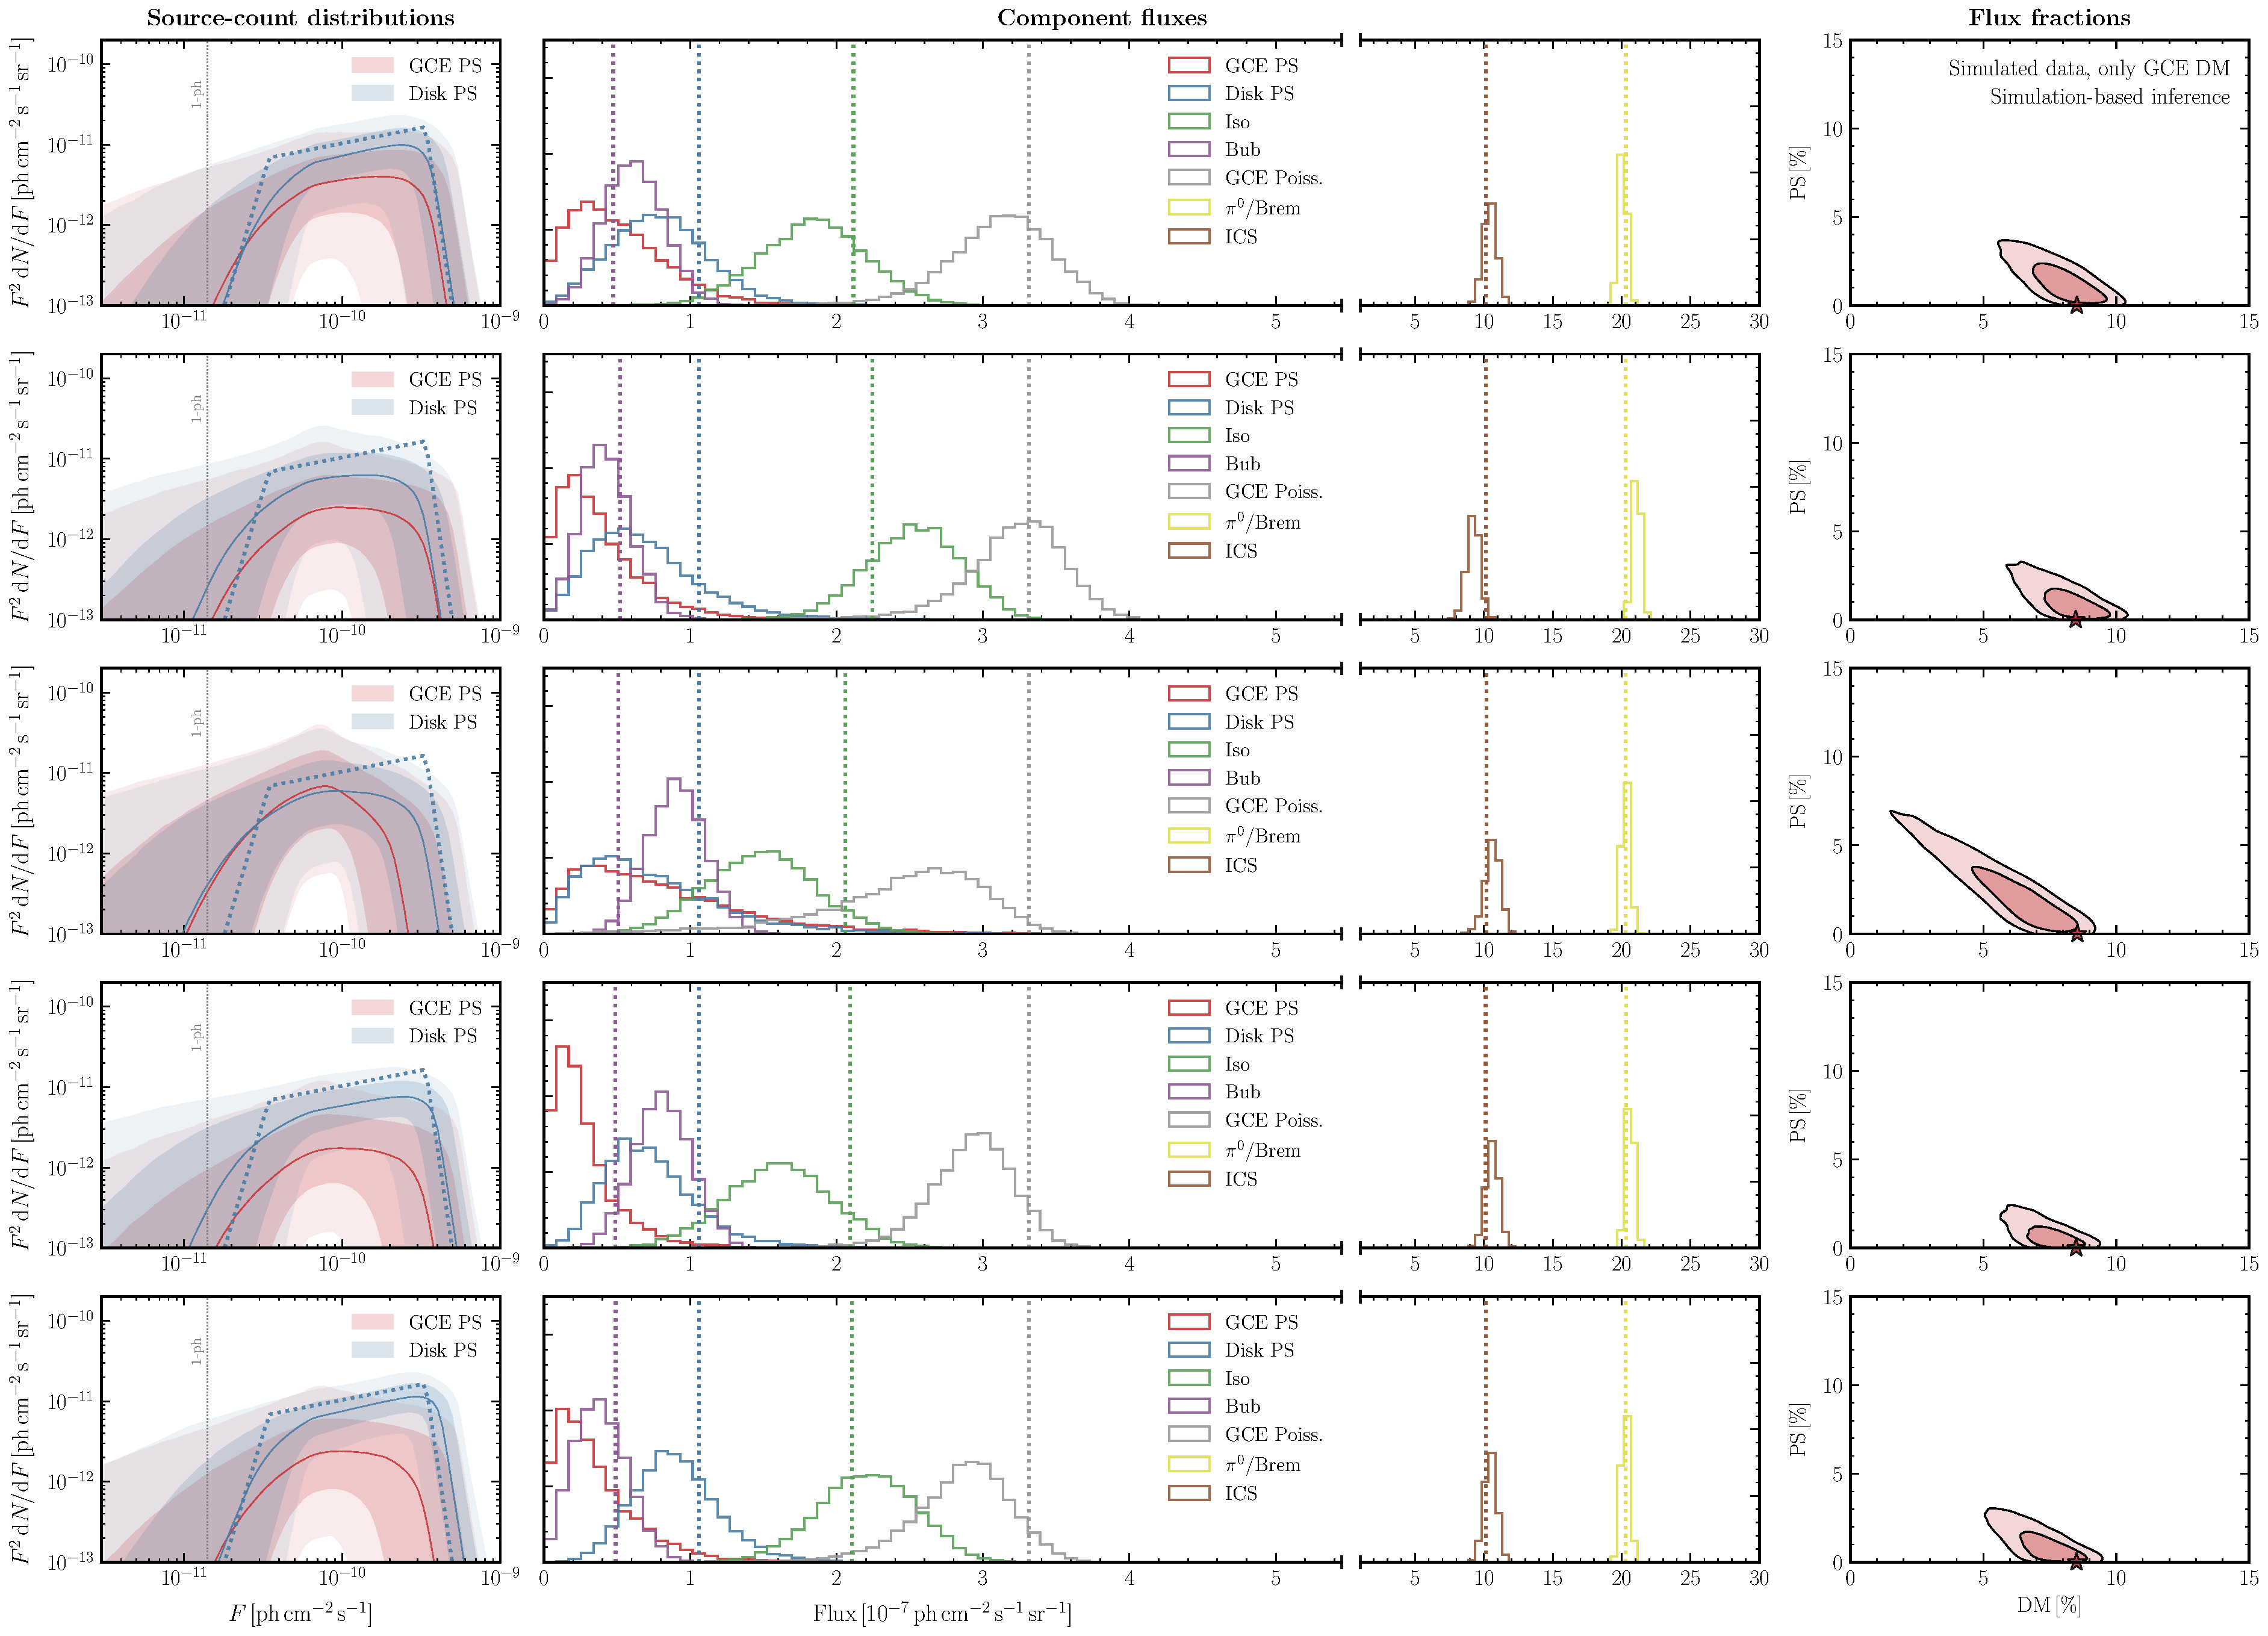
\includegraphics[width=0.95\textwidth]{plots/sim_sbi_dm.pdf}
\caption{Results of the analysis on simulated \Fermi data where the GCE consists of purely DM-like emission, with different rows corresponding to five different simulated realizations. The left column shows the inferred source-count distribution posteriors for GCE-correlated (red) and disk-correlated (blue) PS. Dashed vertical lines corresponding to the flux associated with 1 expected photon count per source and the approximate 1-$\sigma$ threshold for detecting individual sources are given for reference. Solid lines correspond to the inferred median, and the lighter and darker bands represent the middle-68\% and 95\% posterior containments respectively, evaluated point-wise in flux $F$. The middle panel shows the posteriors for the Poissonian templates. The right panel shows the joins posterior on the flux fractions of DM-like and PS-like emission. The dotted lines (in the left two columns) and the stars (in the right column) correspond to the true simulated quantities. DM-like emission is successfully inferred in each case, with the other parameter posteriors corresponding faithfully to the true simulated values.} 
\label{fig:sim_sbi_dm}
\end{figure*}
%

\section{Tests on simulated data}
\label{sec:simulations}

We begin by validating our pipeline on simulated \Fermi data. We create simulated datasets with the parameters of interest in the forward model fixed to posterior medians obtained in a fit of the baseline model to real \Fermi data, and test the ability of our model to infer the presence of either DM-like or PS-like signals on top of the modeled astrophysical background.

Figure~\ref{fig:sim_sbi_dm} shows results of the analysis pipeline conditioning the trained baseline model on five simulated realizations of maps where the GCE consists of purely DM-like emission. The left column shows the median (solid lines) as well as middle-68/95\% containment (dark/light shaded regions) of the posteriors on the source-count distributions $F^2 \dd N/\dd F$ of GCE-correlated (red) and disk-correlated (blue) PS emission, evaluated point-wise in flux $F$. The dashed grey vertical lines correspond to the flux associated with a single expected photon count per source (below which Poissonian and PS-like emission is expected to be perfectly degenerate) and the approximate 1-$\sigma$ threshold for detecting individual sources (below which the degeneracy is often observed in practice~\cite{Chang:2019ars,Buschmann:2020adf}). The middle column shows the posteriors on various modeled emission components, excluding emission from resolved 3FGL PSs as the posterior in that case is largely unconstrained owing to the fact that resolved PSs are masked out in the analysis. The right column shows the joint posterior on the fraction of DM- and PS-like emission in proportion to the total inferred flux in the ROI. The true underlying parameter values from which the data was generated are represented by dotted lines in the left and middle columns, and by star markers in the right column. We see that, in all cases shown, the pipeline successfully recovers the presence of DM-like emission, with little flux---$\lesssim 10\%$ of the total inferred GCE emission in all cases---attributed to PSs. 
%Some PS-like emission is inferred in most cases as well however, due to a combination of degeneracy with both disk-correlated PSs as well as DM-like flux. 
The overall flux of all modeled components is seen to be consistent with the true values used for the simulations.

Figure~\ref{fig:sim_sbi_ps} shows the corresponding results for simulated data containing PS-like emission correlated with the GCE. Here, simulations were produced such that the highest break of the GCE-correlated PS SCD was contained between 5 and 20 expected photon counts. We see that PS-like emission is successfully inferred in each case, while at the same time exemplifying a degeneracy with the Poissonian component. Furthermore, as seen in the left column, the method is able to characterize the contribution of the two modeled PS components through the inferred source-count distribution. Some degeneracy between GCE- and disk-correlated PSs is seen, although the true SCDs are seen to lie within the 95\% posterior containment interval of the inferred source-count distributions in each case.

%
\begin{figure*}
\centering
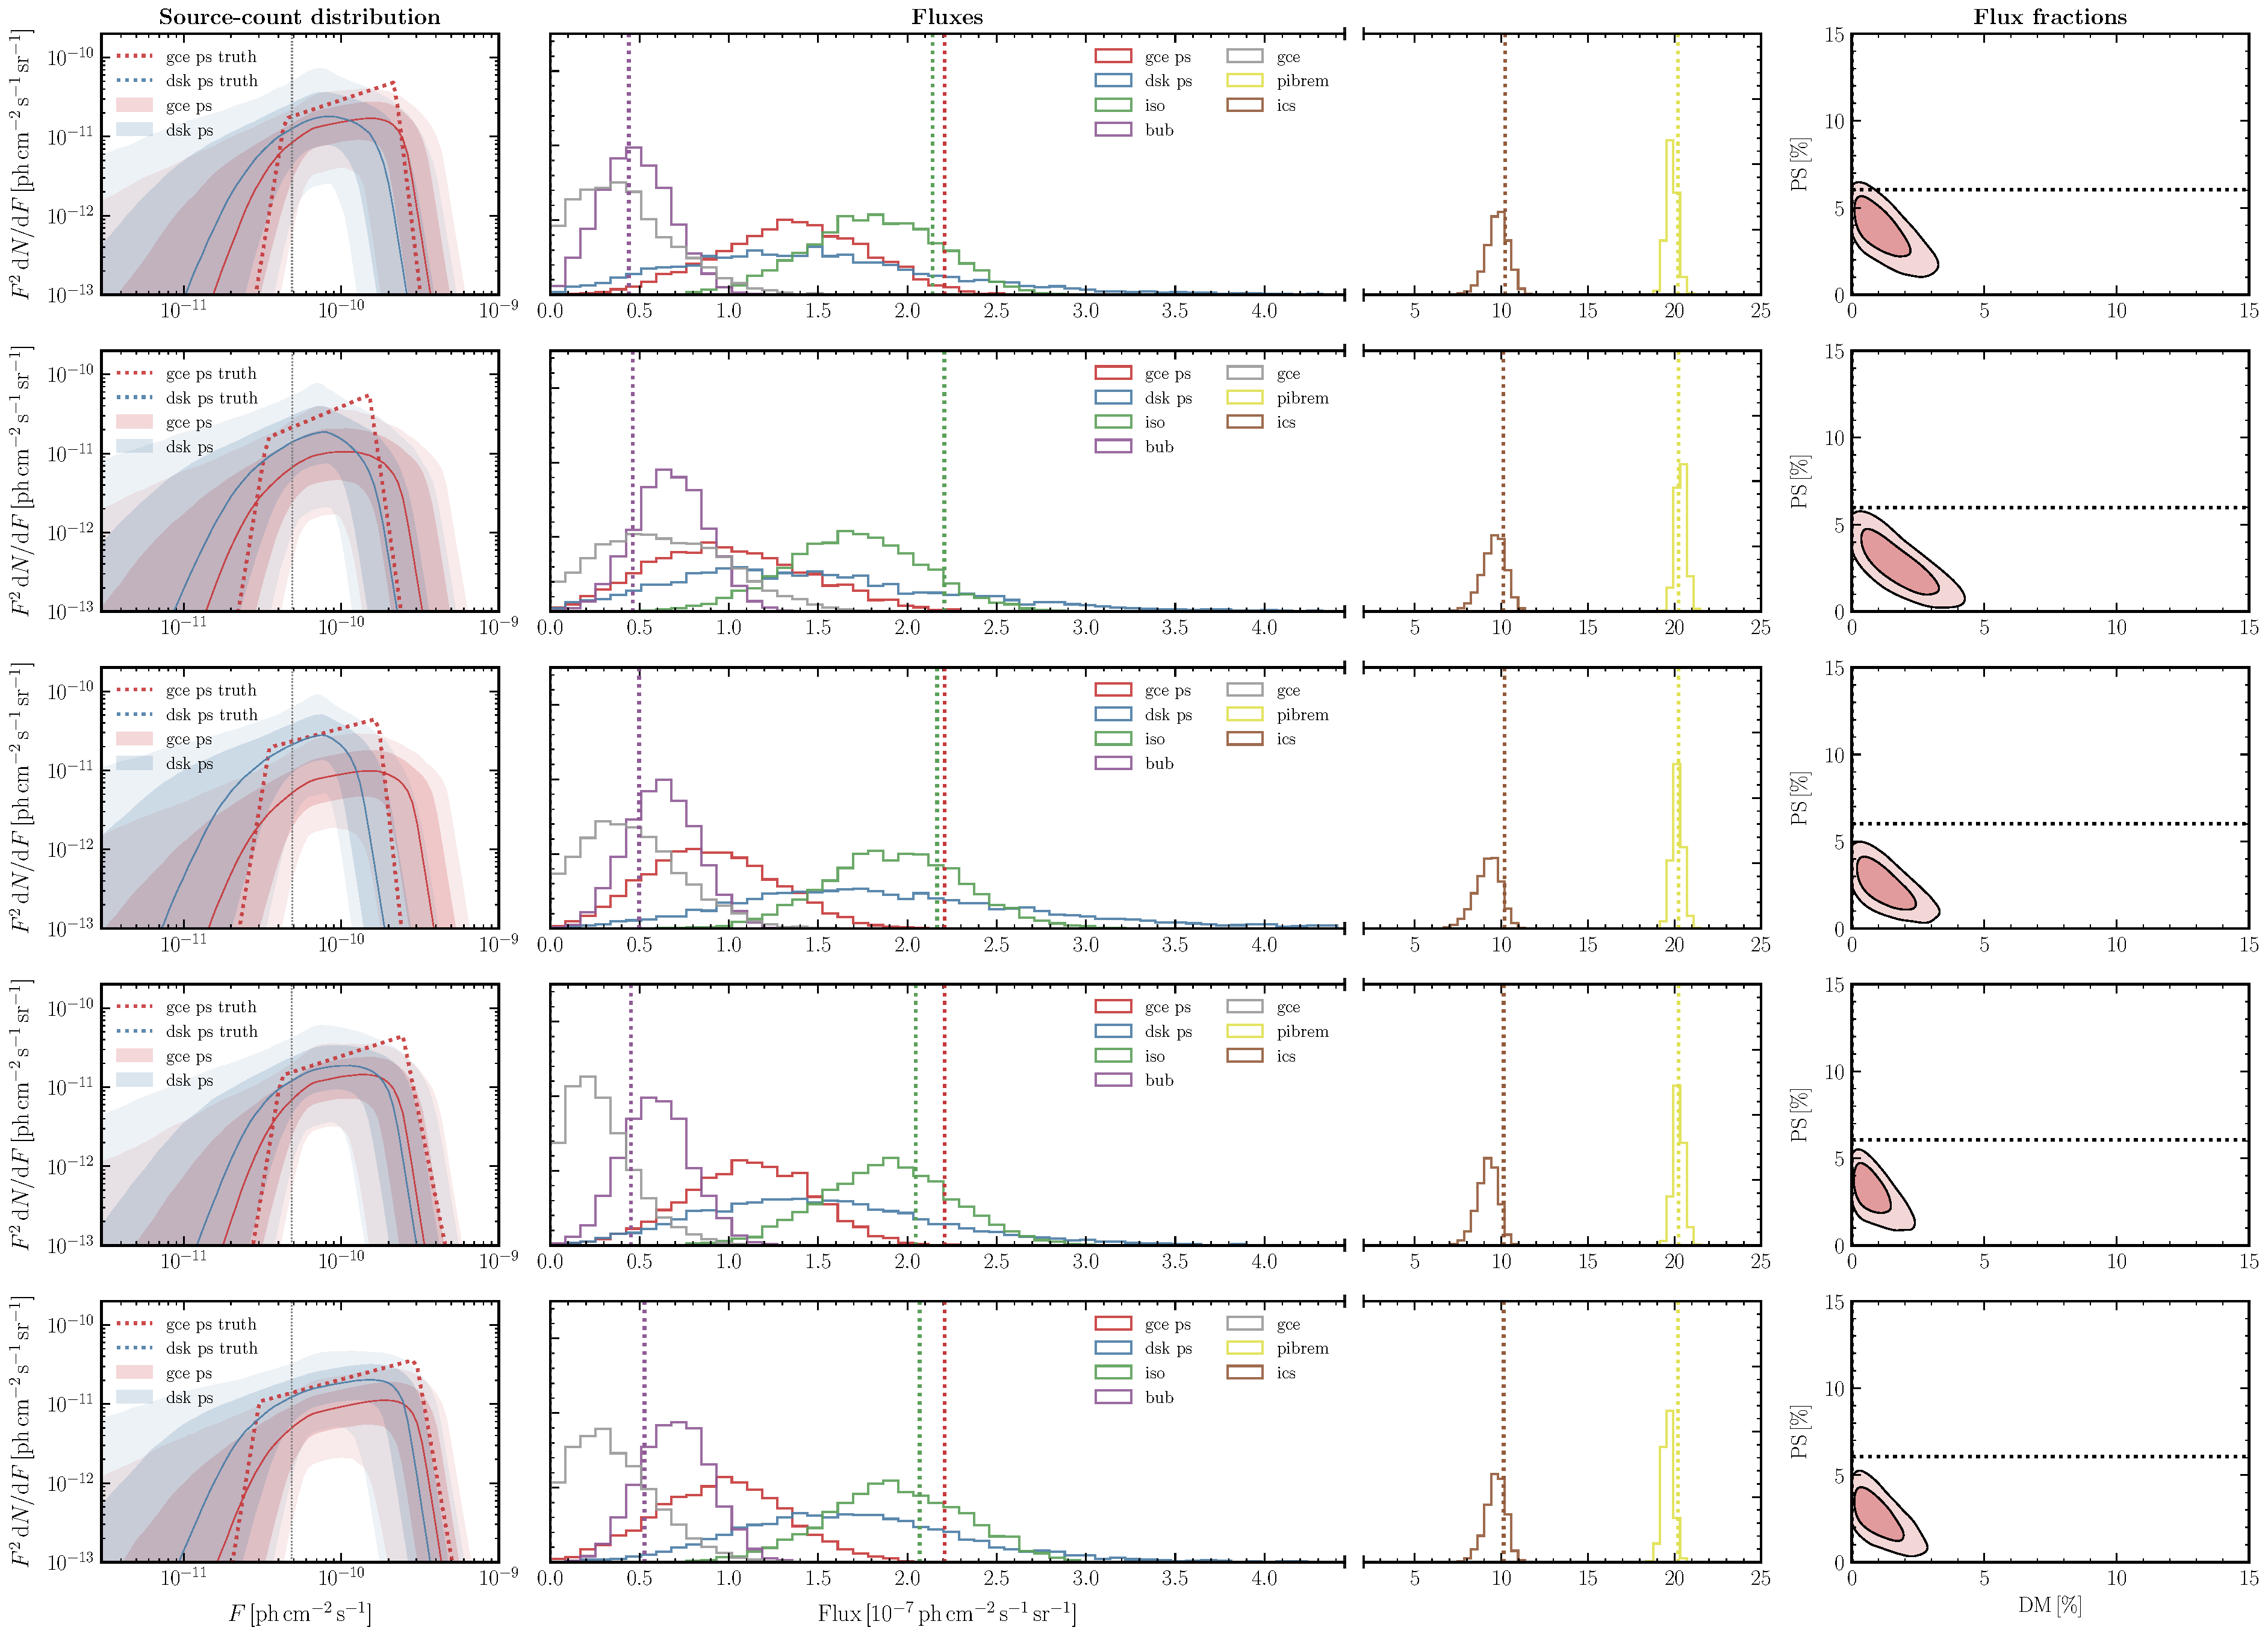
\includegraphics[width=0.95\textwidth]{plots/sim_sbi_ps.pdf}
\caption{Same as Fig.~\ref{fig:sim_sbi_dm}, but for five simulated realization of \Fermi data where the GCE consists of predominantly PS-like emission. PS-like emission is inferred in each case, with the other posteriors corresponding faithfully to their true simulated quantities. The GCE-correlated source-count distribution is also seen to be successfully recovered in the left panel.}
\label{fig:sim_sbi_ps}
\end{figure*}
%

\section{Results on \Fermi data}
\label{sec:data}

We finally apply our neural simulation-based inference pipeline to the real \Fermi dataset. As a point of comparison, we also run the NPTF method described in Sec.~\ref{sec:likelihood-methods} on the data using the same spatial templates and prior assumptions as those used in the corresponding SBI analyses. A summary of the results obtained for different analysis configurations, corresponding to re-training the model using a different set of spatial templates, is shown in Table~\ref{tab:results}, including the fraction of overall emission attributed to the GCE, fraction of the GCE attributed to PS-like emission, flux at which the GCE source count distribution peaks, fraction of the overall emission attributed to disk-correlated PSs, and flux at which the disk source count distribution peaks.

The results of the NPTF analysis are shown in the bottom panel of Fig.~\ref{fig:fid_data}. Consistent with previous studies using a similar configuration, a significant fraction of the GCE---$55.0^{+8.8}_{-22.9}\%$--is attributed to PS-like emission.
The top panel of Fig.~\ref{fig:fid_data} shows results using the neural simulation-based analysis pipeline introduced in this paper. Although posteriors for the astrophysical background templates are seen to be broadly consistent with those inferred in the NPTF analysis, the preference for PSs is reduced in this case, with $32.5^{+9.1}_{-18.7}\%$ of the GCE emission being PS-like. We also note that, in both cases, the inferred GCE-correlated source-count distribution peaks at lower values than those inferred in previous NPTF analyses, which have generally found the bulk of expected emission from PSs to lie just below the 3FGL PS detection threshold~\cite{Lee:2015fea} at $\sim2$--$3\times 10^{-10}$\,ph\,cm$^{-2}$\,s$^{-1}$. In this baseline configuration, the SCD peak is constrained to be $2.3^{+1.2}_{-2.2}\times 10^{-11}$\,ph\,cm$^{-2}$\,s$^{-1}$. We note that that the position of the SCD peak is related to the flux at which the largest number of PSs are inferred to lie, rather than a statement about which fluxes the majority of the emission comes from.


%
\begin{table*}[!t]
    \small
    \begin{center}
    \begin{tabular}{cc|cccccc}
    \toprule
    \textbf{Configuration}  & \textbf{Method}  & \textbf{GCE fraction}	 & \textbf{GCE PS fraction}  & $F_{\mathrm{b}, 1}^\mathrm{GCE}\times 10^{10}$	&  \textbf{Disk PS fraction} &  $F_{\mathrm{b}, 1}^\mathrm{Disk}\times 10^{10}$	&  \textbf{Posteriors}\Tstrut\Bstrut	\\   
    - & - & - & - & [ph\,cm$^{-2}$\,s$^{-1}$] & - & [ph\,cm$^{-2}$\,s$^{-1}$]	& -\Tstrut\Bstrut	\\   
    \Xhline{1\arrayrulewidth}
    \multirow{2}{*}{Baseline} & SBI & $7.8^{+0.2}_{-0.6}\%$ & $38.0^{+8.7}_{-19.2}\%$ & $1.3^{+0.2}_{-0.4}$ & $5.0^{+0.5}_{-1.1}\%$ & $2.2^{+0.2}_{-0.5}$ & \multirow{2}{*}{Figure~\ref{fig:fid_data}}\Tstrut \\
    & NPTF & $7.7^{+0.2}_{-0.6}\%$ & $55.0^{+8.8}_{-22.9}\%$ & $1.1^{+0.1}_{-0.2}$ & $5.4^{+0.5}_{-1.1}\%$ & $2.0^{+0.2}_{-0.5}$\Bstrut &\\ 
    \hline
    \multirow{2}{*}{Diffuse Model A} & SBI & $6.4^{+0.2}_{-0.6}\%$ & $47.5^{+9.9}_{-25.1}\%$ & $1.3^{+0.3}_{-0.4}$ & $4.9^{+0.5}_{-1.2}\%$ & $2.4^{+0.2}_{-0.5}$ & \multirow{2}{*}{Figure~\ref{fig:fid_data_modelA}}\Tstrut  \\ 
    & NPTF & $6.7^{+0.2}_{-0.6}\%$ & $74.9^{+6.6}_{-22.5}\%$ & $1.1^{+0.1}_{-0.2}$ & $5.1^{+0.5}_{-1.3}\%$ & $2.2^{+0.2}_{-0.5}$\Bstrut &\\
    \hline
    \multirow{2}{*}{Diffuse Model F} & SBI & $4.7^{+0.2}_{-0.6}\%$ & $62.2^{+10.2}_{-26.4}\%$ & $1.5^{+0.3}_{-0.5}$ & $5.2^{+0.5}_{-1.1}\%$ & $2.5^{+0.2}_{-0.5}$
    & \multirow{2}{*}{Figure~\ref{fig:fid_data_modelF}}\Tstrut \\
    & NPTF & $5.2^{+0.2}_{-0.5}\%$ & $67.5^{+8.6}_{-26.7}\%$ & $1.1^{+0.2}_{-0.3}$ & $6.4^{+0.5}_{-1.1}\%$ & $2.0^{+0.2}_{-0.4}$\Bstrut &\\
    \hline
    \multirow{2}{*}{Thick disk} & SBI & $7.9^{+0.3}_{-0.6}\%$ & $51.9^{+8.5}_{-22.2}\%$ & $1.4^{+0.2}_{-0.4}$ & $3.2^{+0.5}_{-1.2}\%$ & $2.5^{+0.3}_{-0.6}$ & \multirow{2}{*}{Figure~\ref{fig:fid_data_thick_disk}}\Tstrut \\
    & NPTF & $8.2^{+0.3}_{-0.7}\%$ & $75.0^{+7.1}_{-22.6}\%$ & $1.1^{+0.1}_{-0.2}$ & $2.3^{+0.7}_{-1.1}\%$ & $3.1^{+0.6}_{-1.2}$\Bstrut &\\
    \botrule
    \end{tabular}
    \end{center}
    \caption{Inferred values for the GCE flux as a fraction of the total flux, the GCE PS-like flux as a fraction of the total GCE flux, the position of the upper source count flux break $F_{\mathrm{b}, 1}$ for the GCE and disk PS components, and the disk flux as a fraction of the total flux. For the baseline configuration as well as the various systematic variations explored, the median along with the 16th and 84th posterior percentile values are shown for the simulation-based inference and NPTF analyses.}
    \label{tab:results}
    \end{table*}    
    %

%
\begin{figure*}
\centering
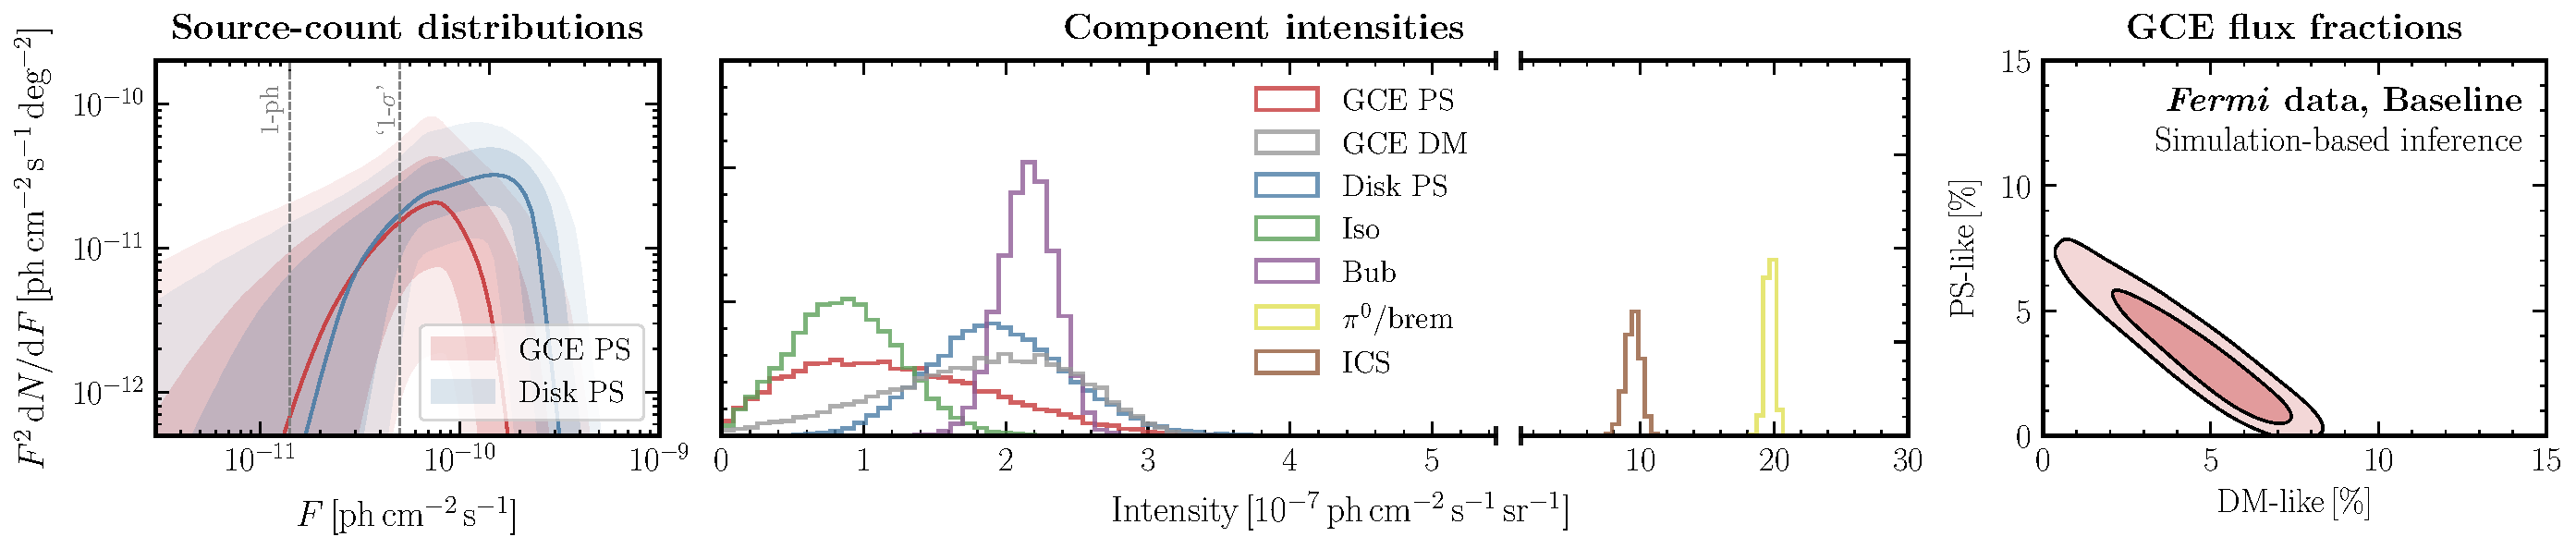
\includegraphics[width=0.95\textwidth]{plots/data_fid_sbi.pdf}
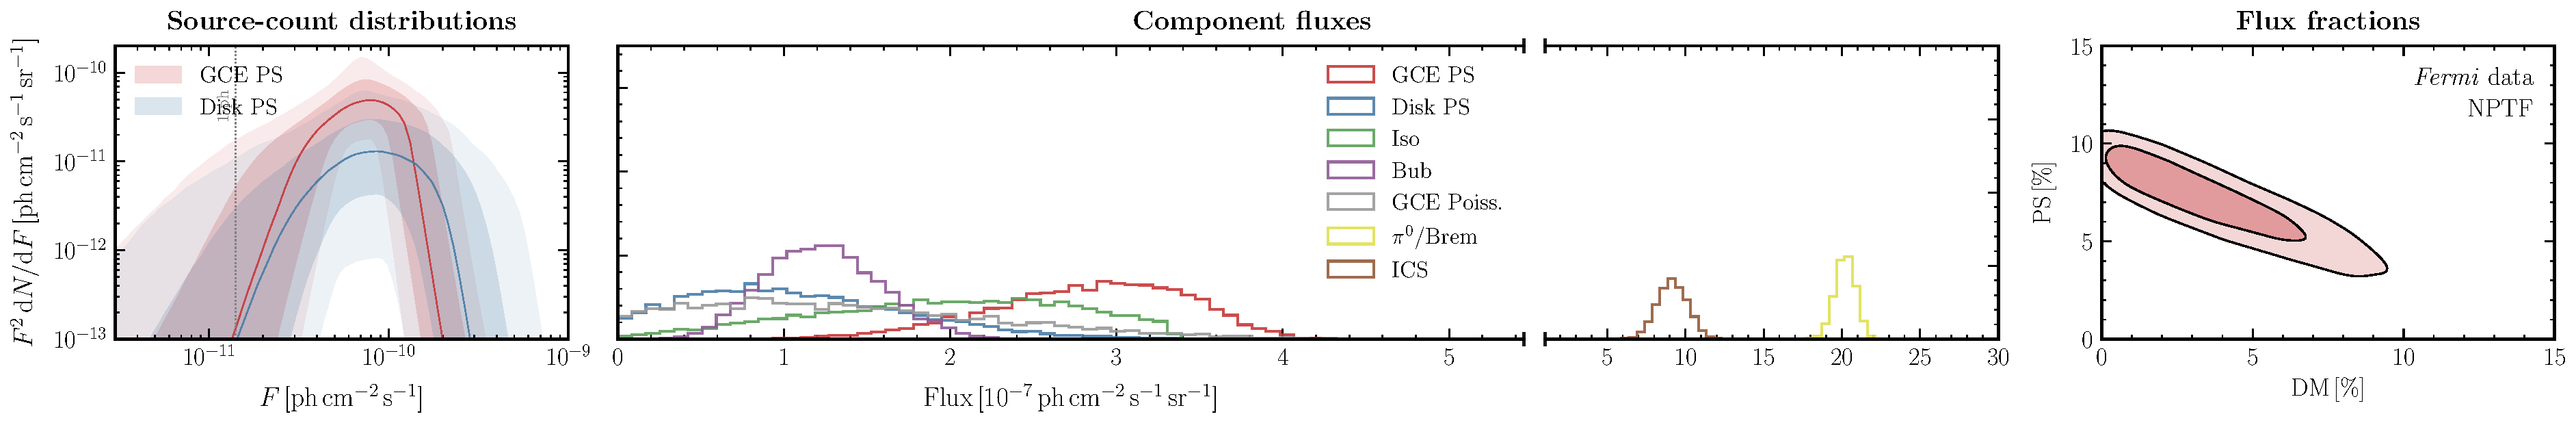
\includegraphics[width=0.95\textwidth]{plots/data_fid_nptf.pdf}
\caption{Results of the baseline analysis on real \Fermi data. \emph{(Top row)} Analysis using neural simulation-based inference with normalizing flows, and \emph{(bottom row)} using the 1-point PDF likelihood implemented in the non-Poissonian template fitting (NPTF) framework. While moderate preference for a PS-like origin of the GCE is seen in the case of the NPTF analysis (bottom), the simulation-based inference analysis attributes a smaller fraction of the GCE to PS-like emission (top).}
\label{fig:fid_data}
\end{figure*}
%

\subsection{Signal injection test on data}
\label{sec:sig-injection}

A crucial test of self-consistency is the ability of the method to recover an artificial signal injected onto the real $\gamma$-ray data. As shown in Ref.~\cite{Leane:2019xiy}, initial applications of the NPTF to the GCE would generally fail this closure test, with implications for characterizing the nature of PSs in the Galactic Center explored in Refs.~\cite{Chang:2019ars,Buschmann:2020adf}. In particular, it was shown that this test can help diagnose underlying issues associated with mismodeling of the diffuse foreground emission, which have the potential to bias the characterization of PS populations. Recent NPTF analyses using improved descriptions of foreground modeling~\cite{Buschmann:2020adf} show consistent behavior under the closure test. We perform a version of this test within our framework, testing the ability of our method to recover different mock signals injected onto the real \Fermi data.

Figure~\ref{fig:sig_inj_data} shows the results of this test, with the different rows corresponding to different signal configurations---purely DM, bright PSs, medium-bright PSs, and dim PSs. Bright, medium-bright, and dim PS configurations are taken have a maximum PS flux (given by the highest break in Eq.~\eqref{eq:scd_bpl}) at 20, 10, and 5 photon counts respectively, with other parameters the same as those inferred on real \Fermi data. The leftmost columns show the baseline analysis on \Fermi data, with subsequent columns showing signals of progressively larger sizes injected onto the data, up to approximately the size of the original GCE signal. The dotted horizontal and vertical lines show the total emissions including the injected signal and the median fluxes for the PS and DM components of the GCE inferred without any additional injected signal, respectively. 

The additional injected signal is seen to be reconstructed correctly within the inferred 95\% confidence interval in all four cases. For the DM signal (top row), the brightest tested DM signal is seen to partially reconstruct as PS-like, which could be attributed to the larger magnitude of Poisson fluctuations in this case mimicking the effect of an unresolved PS population. The injected PS signals (rows 2--4) are correctly reconstructed in all cases, with the dimmer PS signals showing a more prominent flat direction with Poissonian emission, as expected.

%
\begin{figure*}
\centering

\includegraphics[width=0.95\textwidth]{plots/sig_inj_title.pdf}
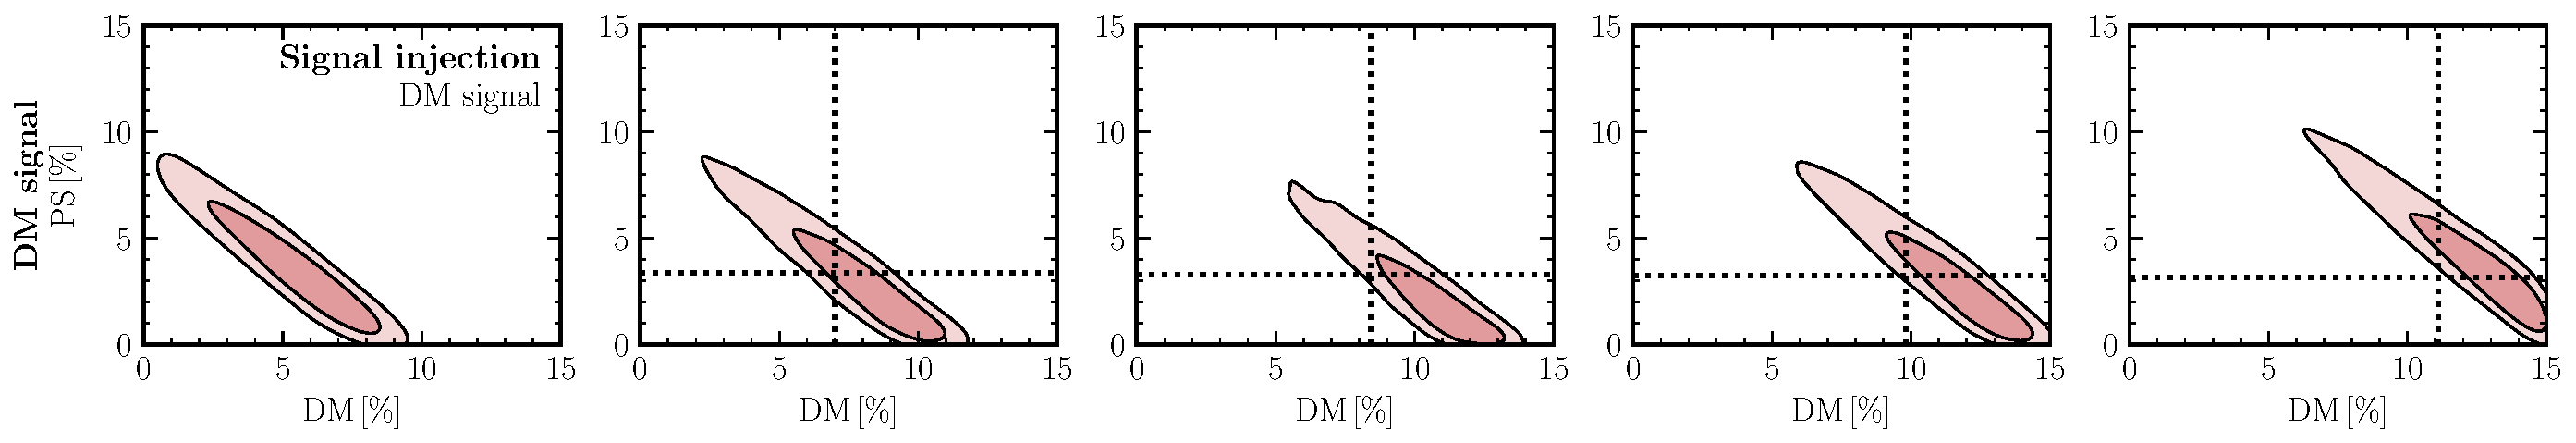
\includegraphics[width=0.95\textwidth]{plots/data_sig_inj_dm.pdf}
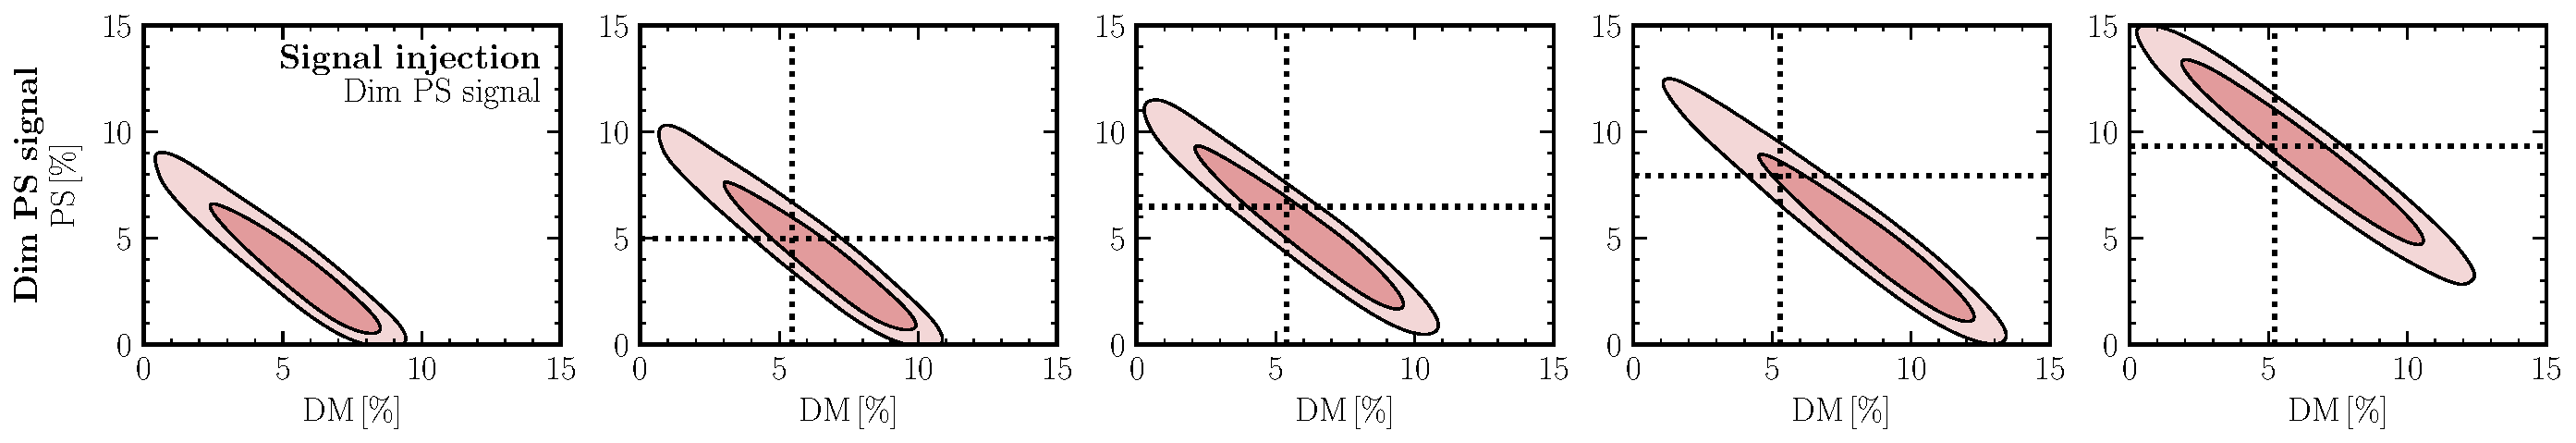
\includegraphics[width=0.95\textwidth]{plots/data_sig_inj_dim_ps.pdf}
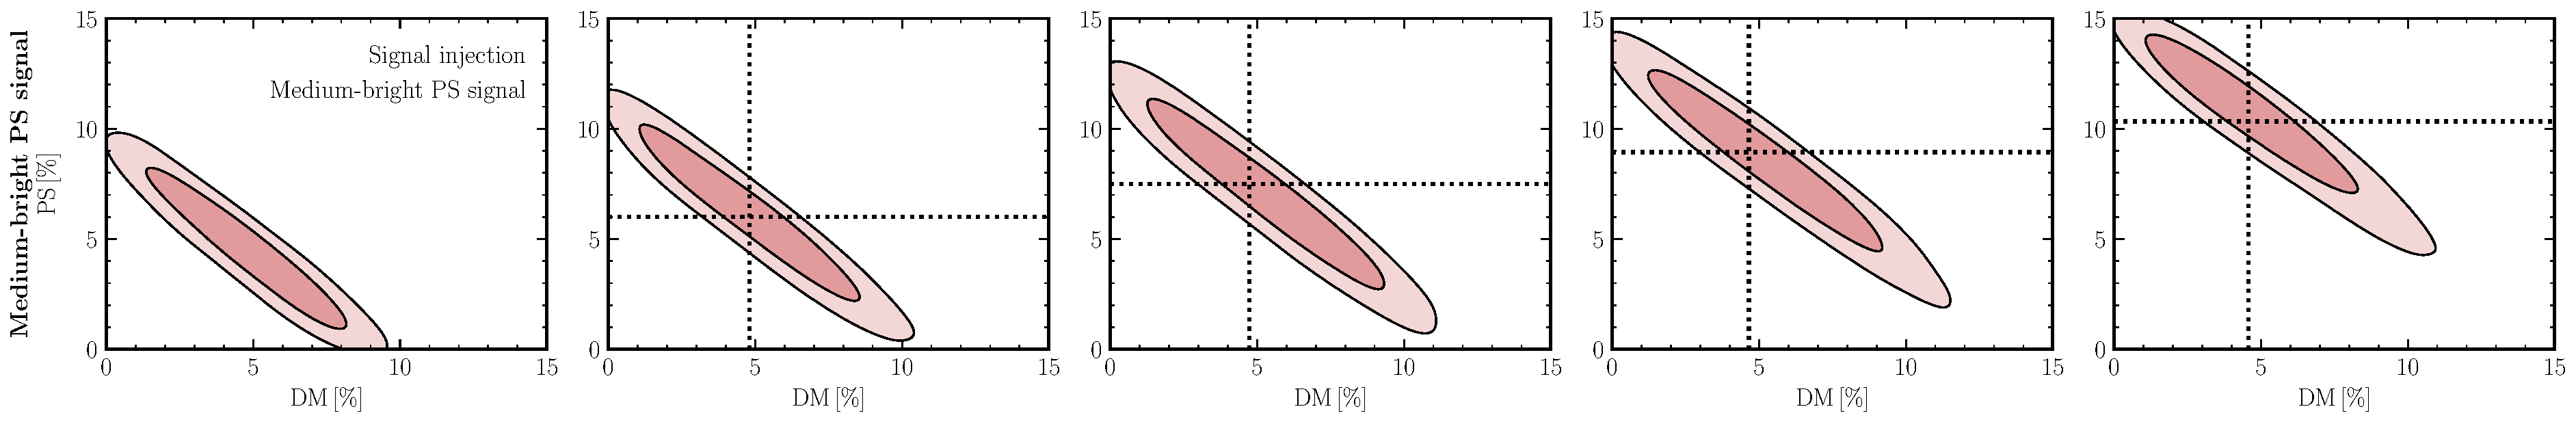
\includegraphics[width=0.95\textwidth]{plots/data_sig_inj_med_ps.pdf}
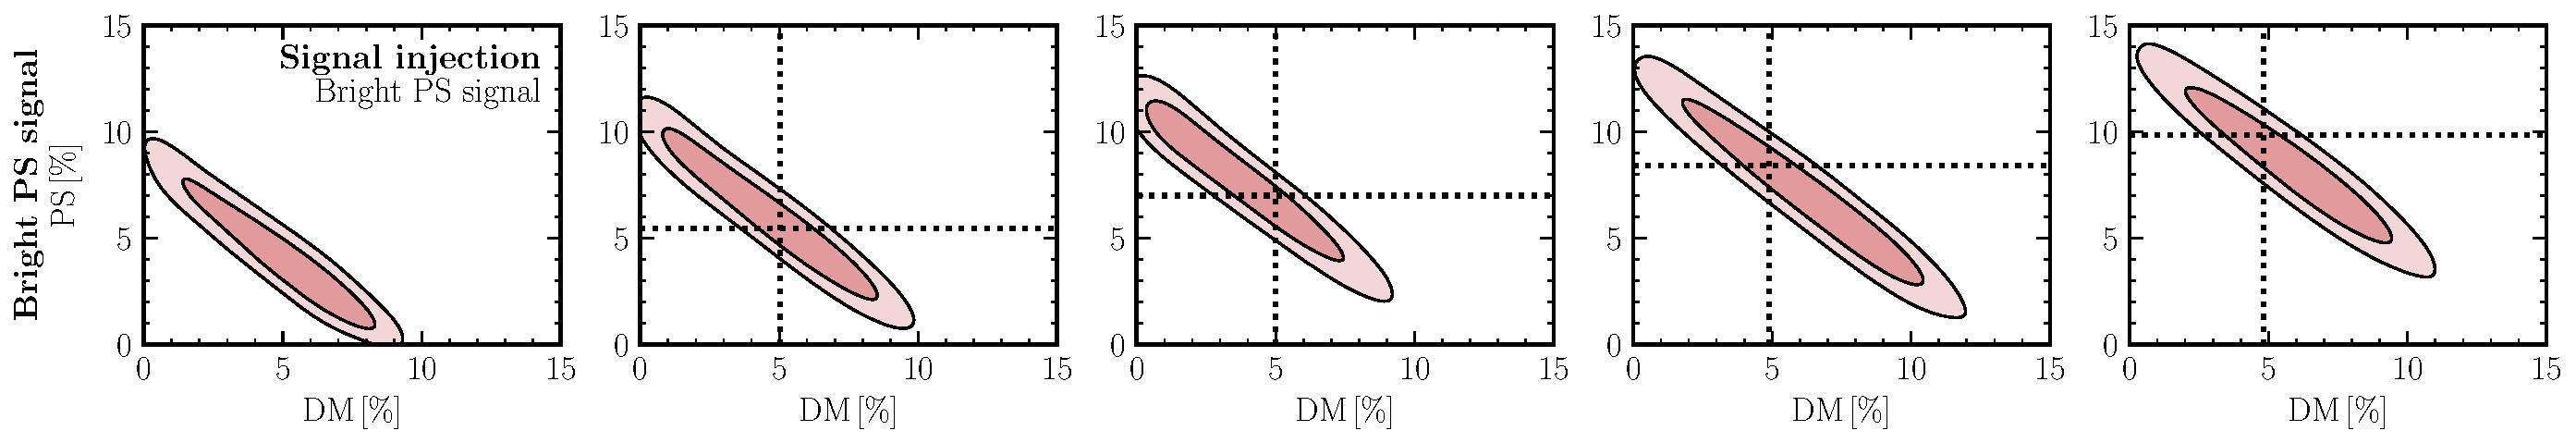
\includegraphics[width=0.95\textwidth]{plots/data_sig_inj_ps.pdf}

\includegraphics[width=0.95\textwidth]{plots/sig_inj_chyron.pdf}
\caption{Joint posterior for the flux fraction of PS-like and DM-like emission when an artificial DM signal is injected onto the real \Fermi data. The different rows correspond to different signal types, from top to bottom, purely DM, dim PSs (maximum of 5 expected counts per PS), moderately-bright PSs (maximum of 10 expected counts per PS), and bright PSs (maximum of 20 expected counts per PS). The leftmost panels shows the baseline analysis on \Fermi data, with subsequent panels showing results with progressively larger signals injected onto the data. The dotted lines show the expected total emissions including the injected signal and the median fluxes. The additional injected DM and PS signals are seen to correctly reconstructed within the respective posterior bounds in all cases.}
\label{fig:sig_inj_data}
\end{figure*}
%

\subsection{Systematic variations on the analysis}
\label{sec:systematics}

% %
% \begin{figure*}
%     \centering
%     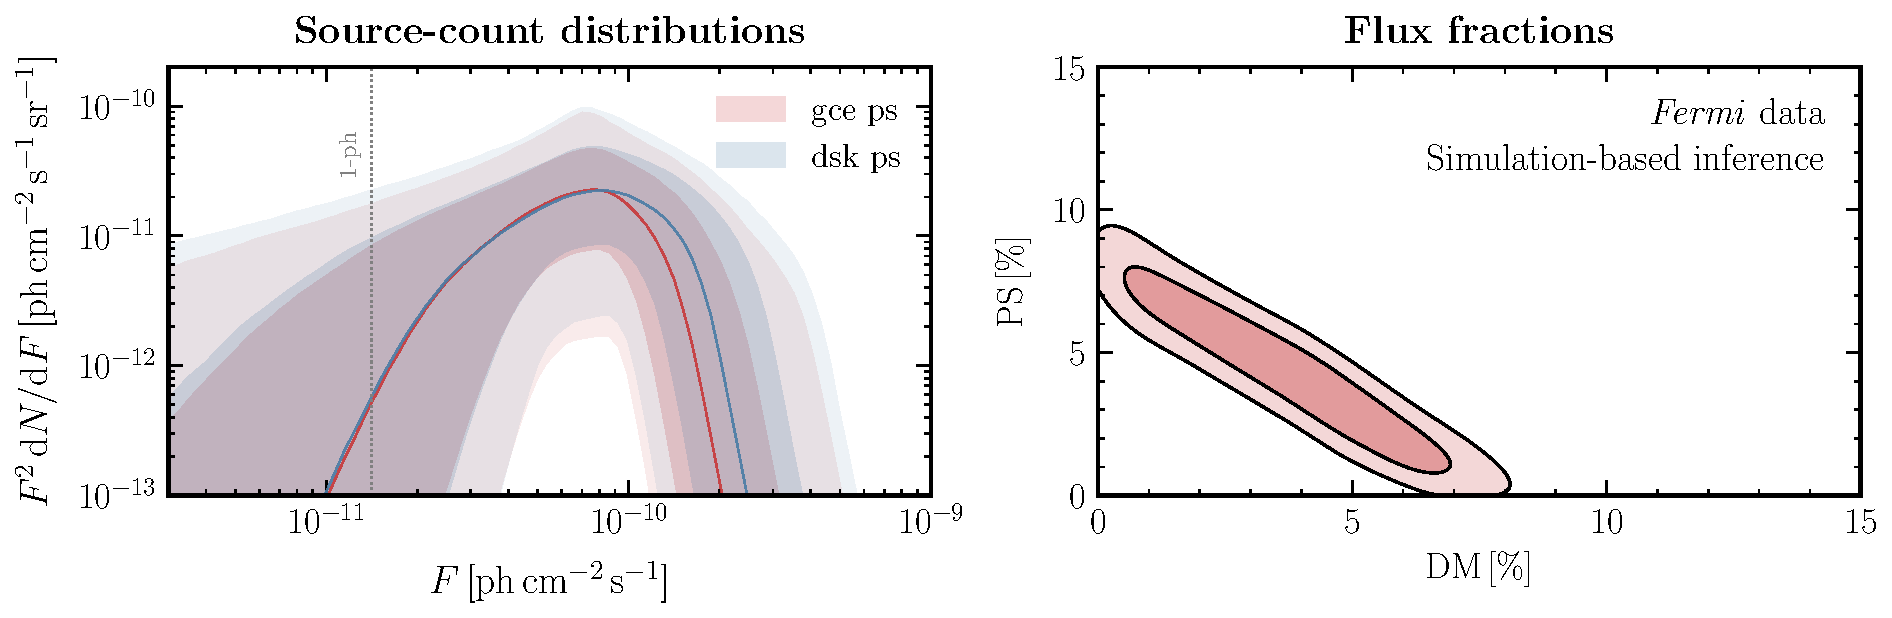
\includegraphics[width=0.45\textwidth]{plots/data_fid_sbi_20.pdf}
%     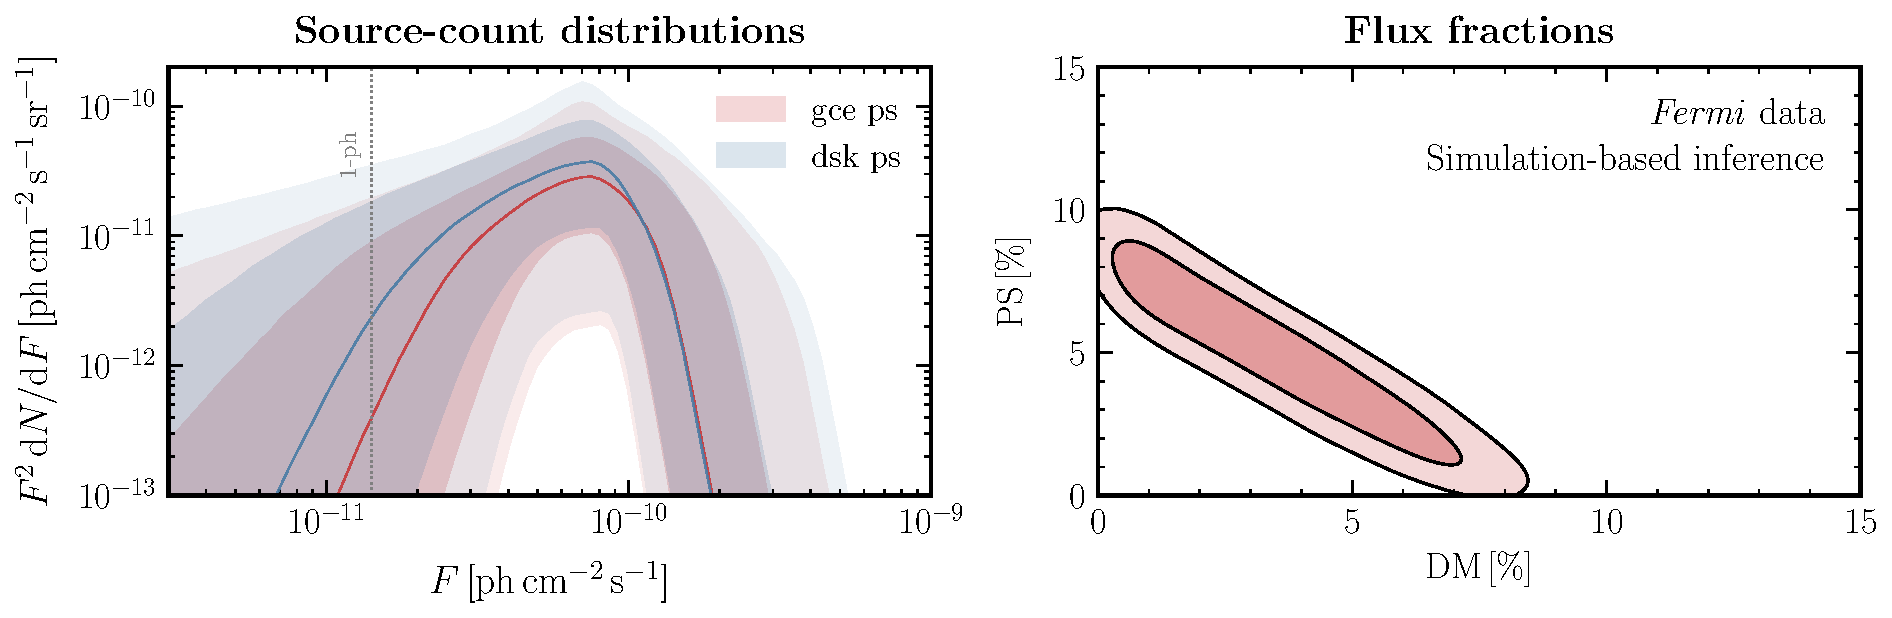
\includegraphics[width=0.45\textwidth]{plots/data_fid_sbi_15.pdf}
%     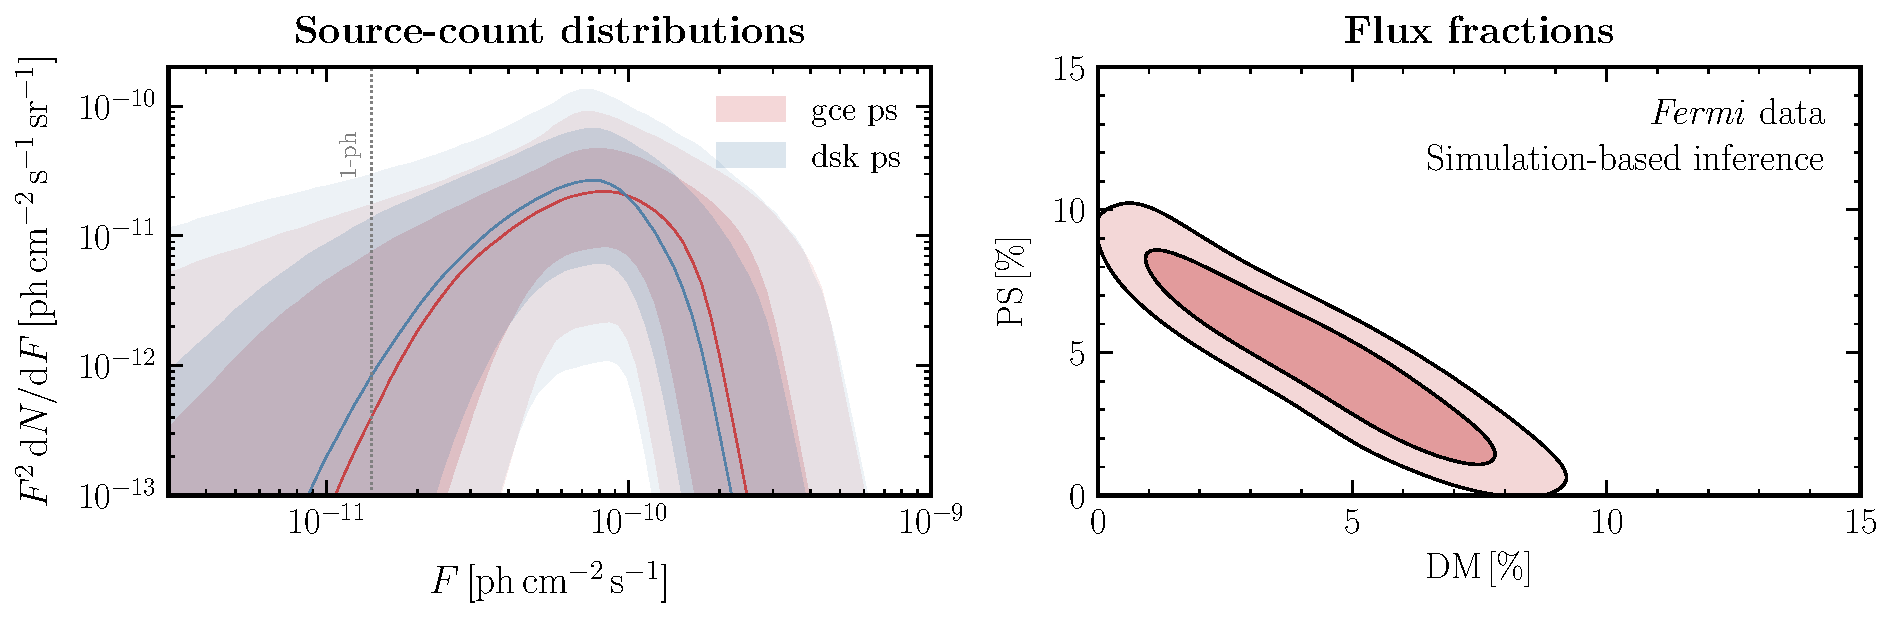
\includegraphics[width=0.45\textwidth]{plots/data_fid_sbi_10.pdf}
%     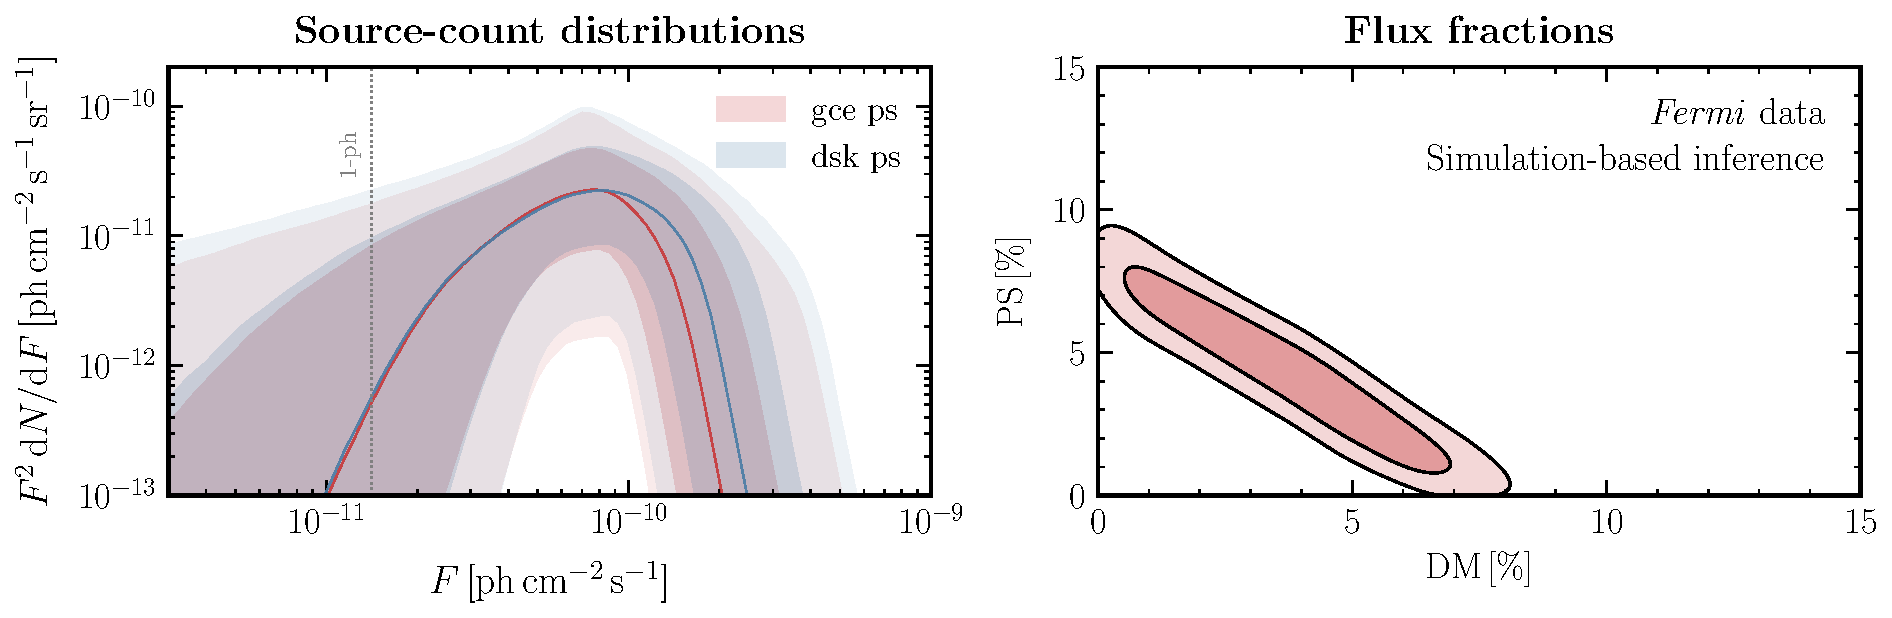
\includegraphics[width=0.45\textwidth]{plots/data_fid_sbi_20.pdf}
%     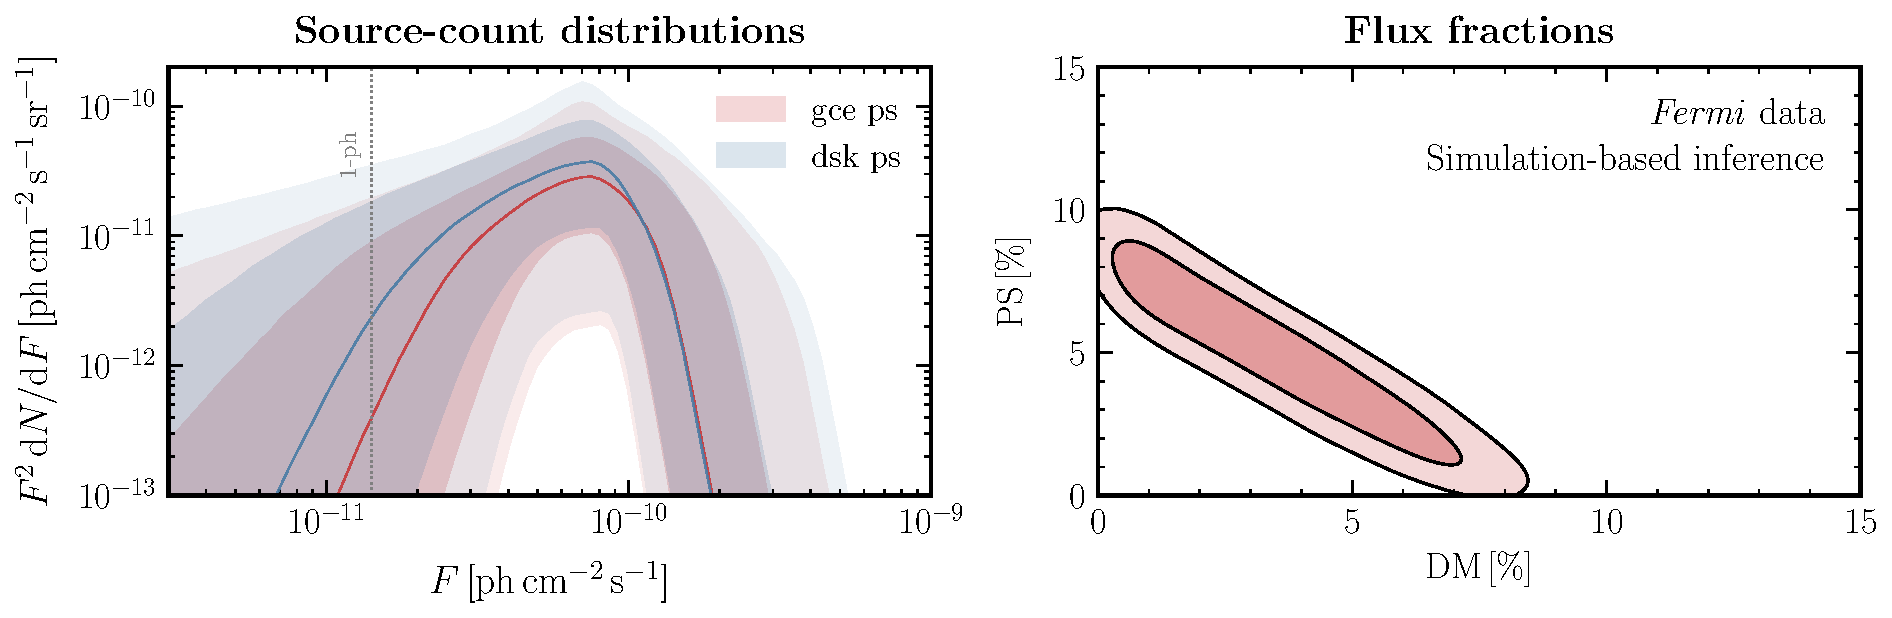
\includegraphics[width=0.45\textwidth]{plots/data_fid_sbi_15.pdf}
%     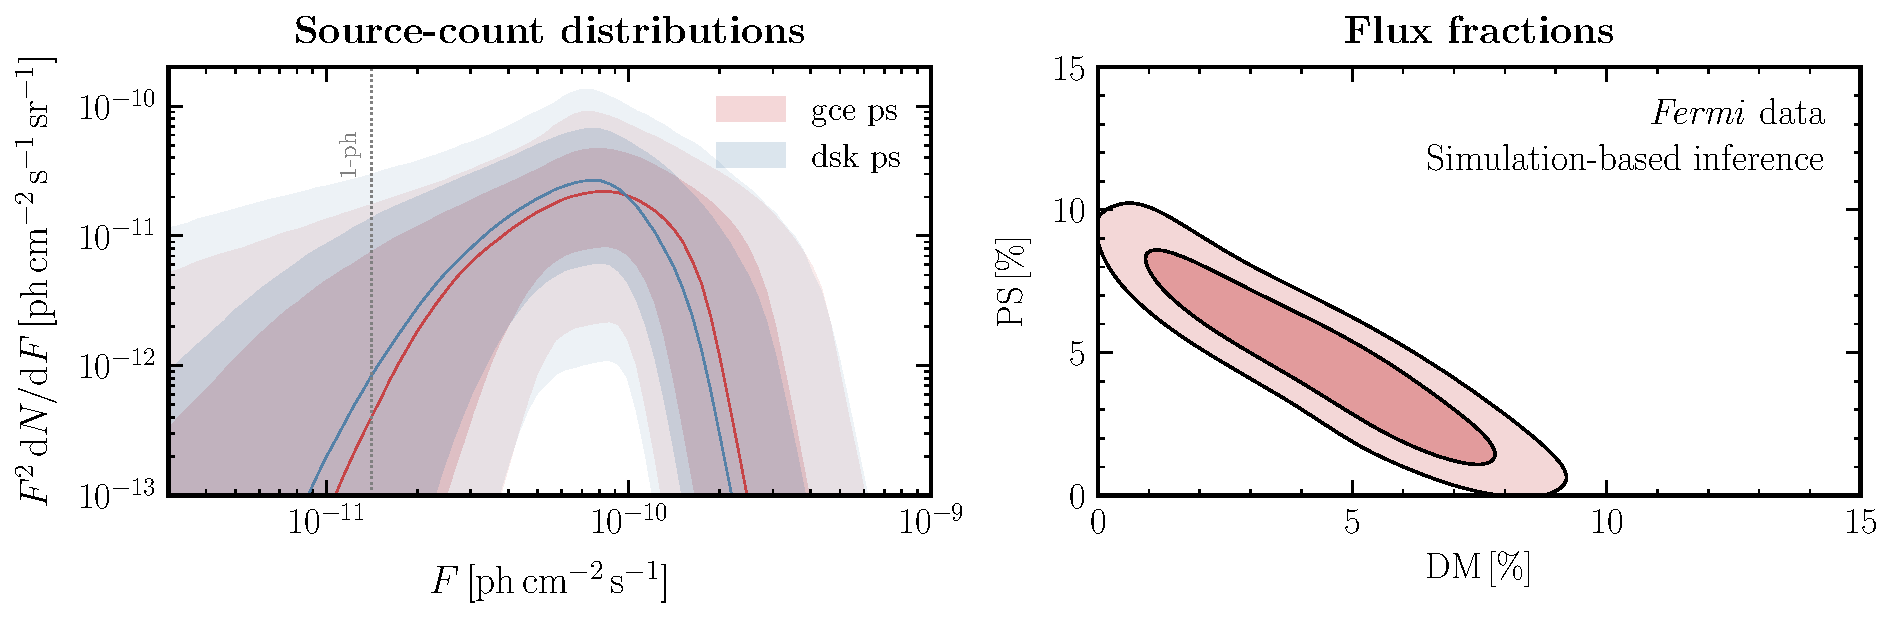
\includegraphics[width=0.45\textwidth]{plots/data_fid_sbi_10.pdf}

%     % 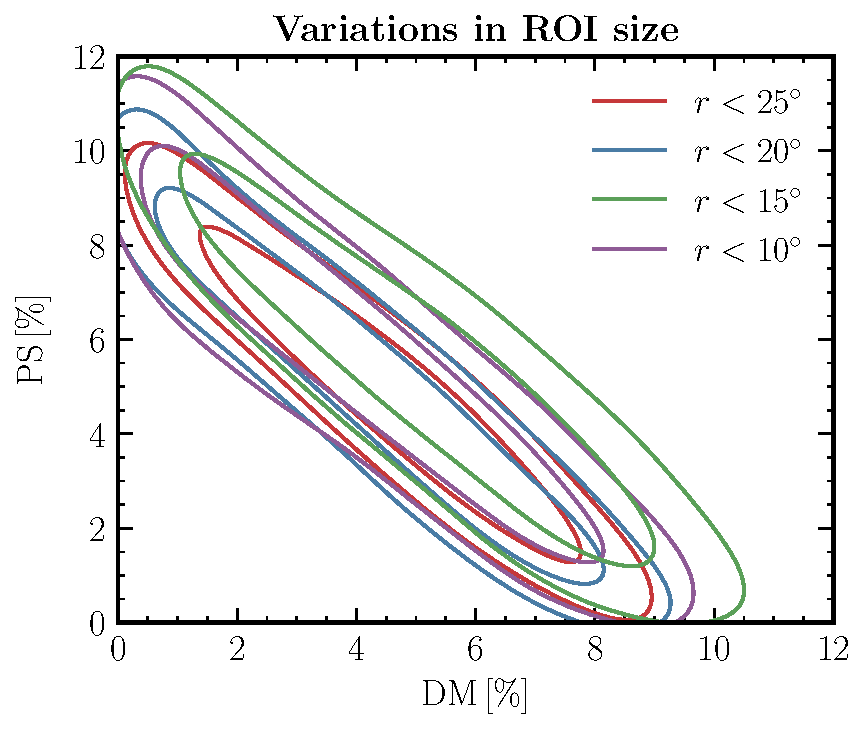
\includegraphics[width=0.22\textwidth]{plots/roi_var.pdf}
%     \caption{Joint posterior for flux fraction of PS-like and DM-like emission on real \Fermi data for different diffuse models \emph{(left)} and ROI sizes \emph{(right)}. In varying diffuse models, the baseline Model O (red) is compared with results obtained using Models A (blue) and F (green). Although the overall GCE flux is seen to varying by up to a factor of $\sim2$ between diffuse models, no evidence for PS-like emission is seen. As seen in the right panel, results remain consistent for smaller ROI sizes.}
%     \label{fig:variations}
% \end{figure*}
% %



%
\begin{figure*}
\centering
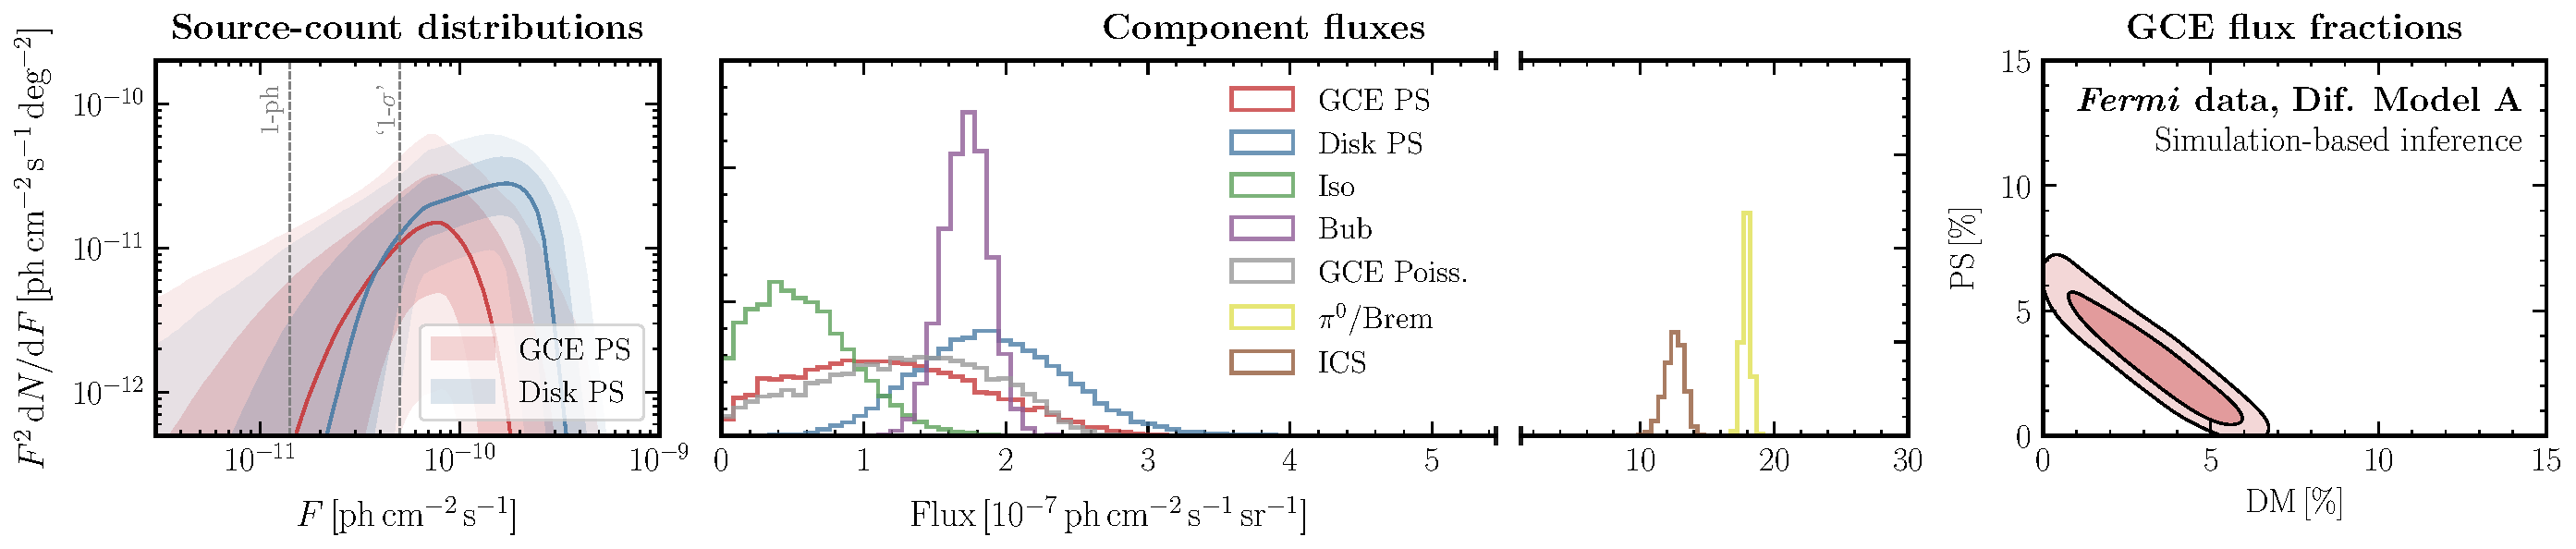
\includegraphics[width=0.95\textwidth]{plots/data_fid_sbi_modelA.pdf}
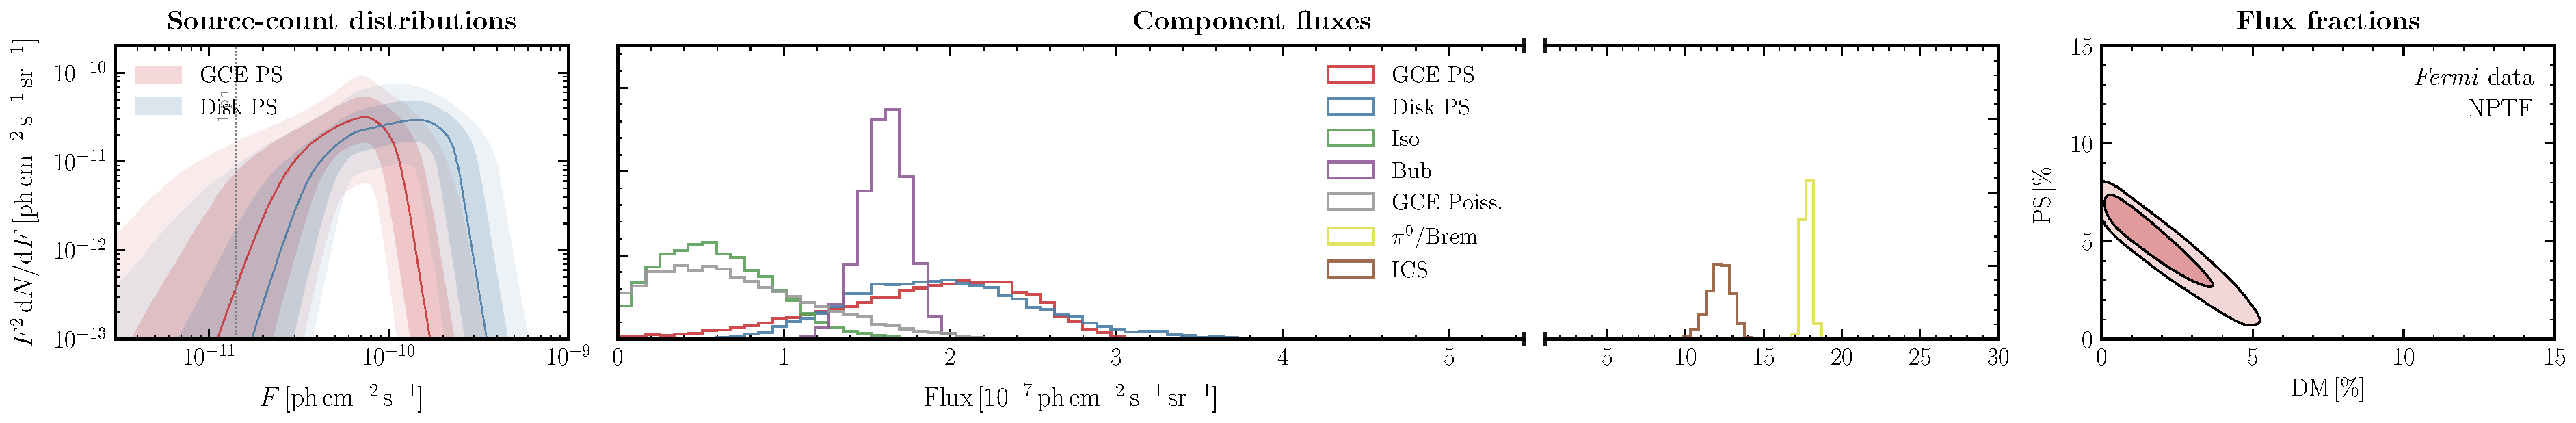
\includegraphics[width=0.95\textwidth]{plots/data_fid_nptf_modelA.pdf}
\caption{Same as Fig.~\ref{fig:fid_data}, but for a model where the diffuse foreground emission is modeled using the alternative Model A.}
\label{fig:fid_data_modelA}
\end{figure*}
%


%
\begin{figure*}
\centering
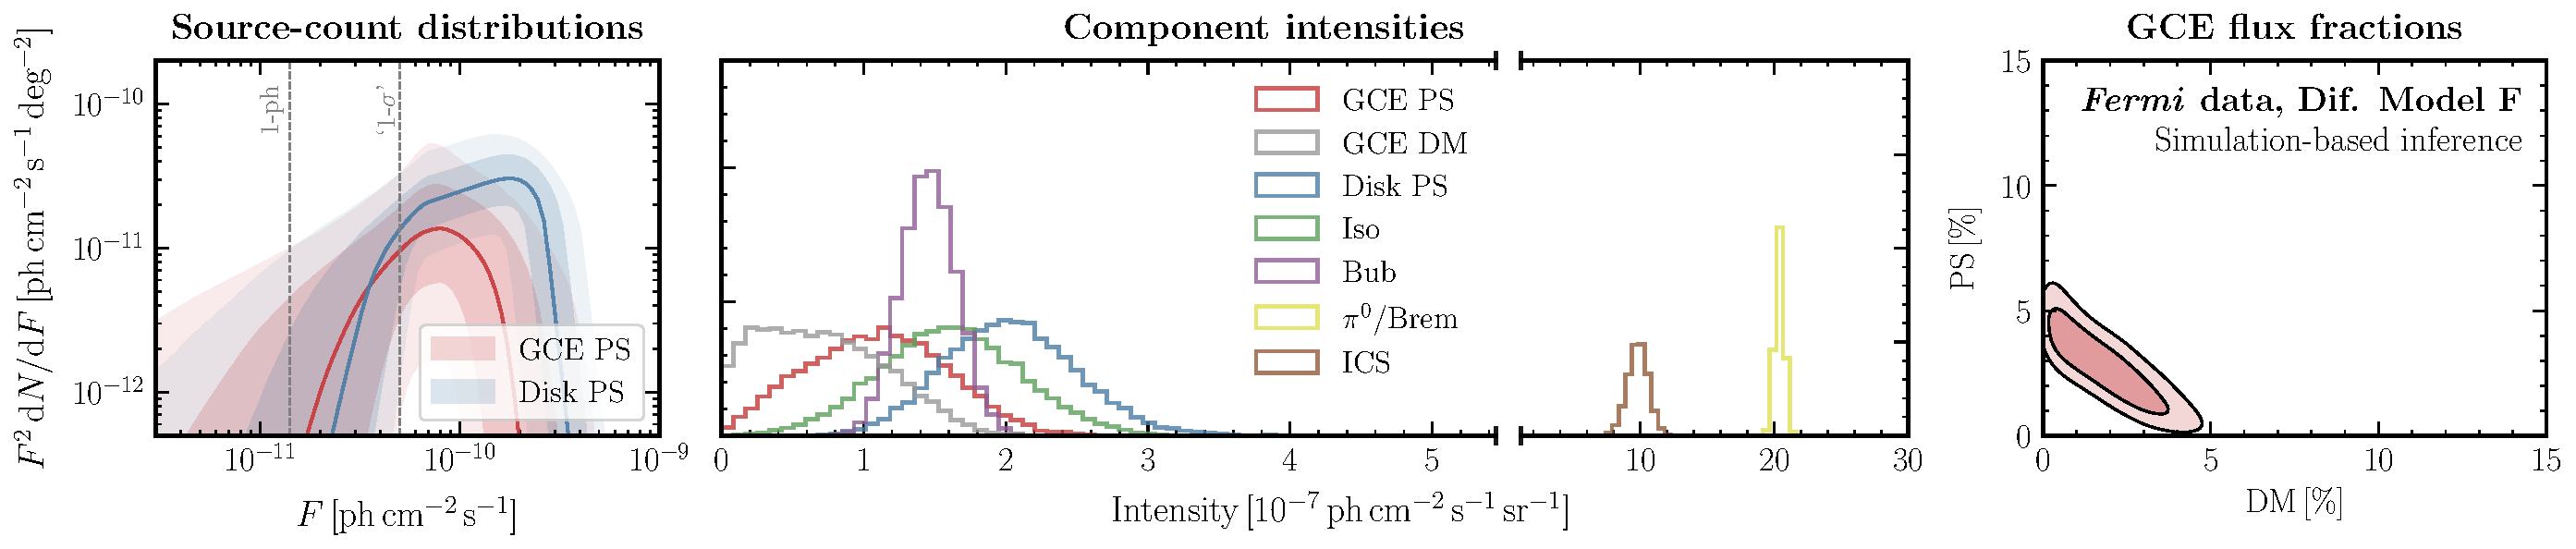
\includegraphics[width=0.95\textwidth]{plots/data_fid_sbi_modelF.pdf}
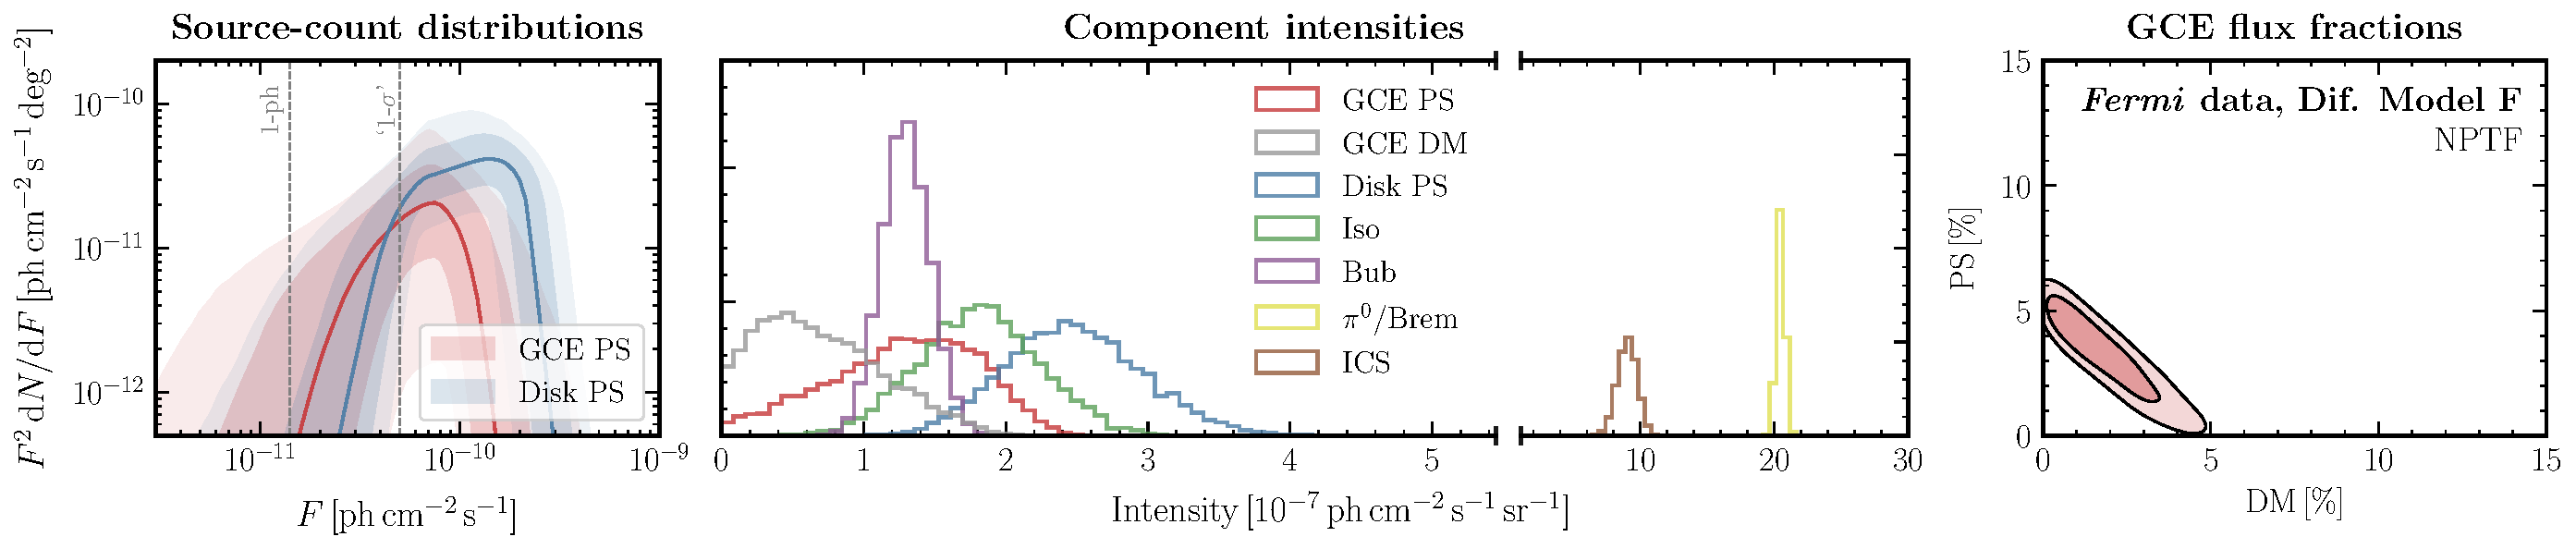
\includegraphics[width=0.95\textwidth]{plots/data_fid_nptf_modelF.pdf}
\caption{Same as Fig.~\ref{fig:fid_data}, but for a model where the diffuse foreground emission is modeled using the alternative Model F.}
\label{fig:fid_data_modelF}
\end{figure*}
%

%
\begin{figure*}
\centering
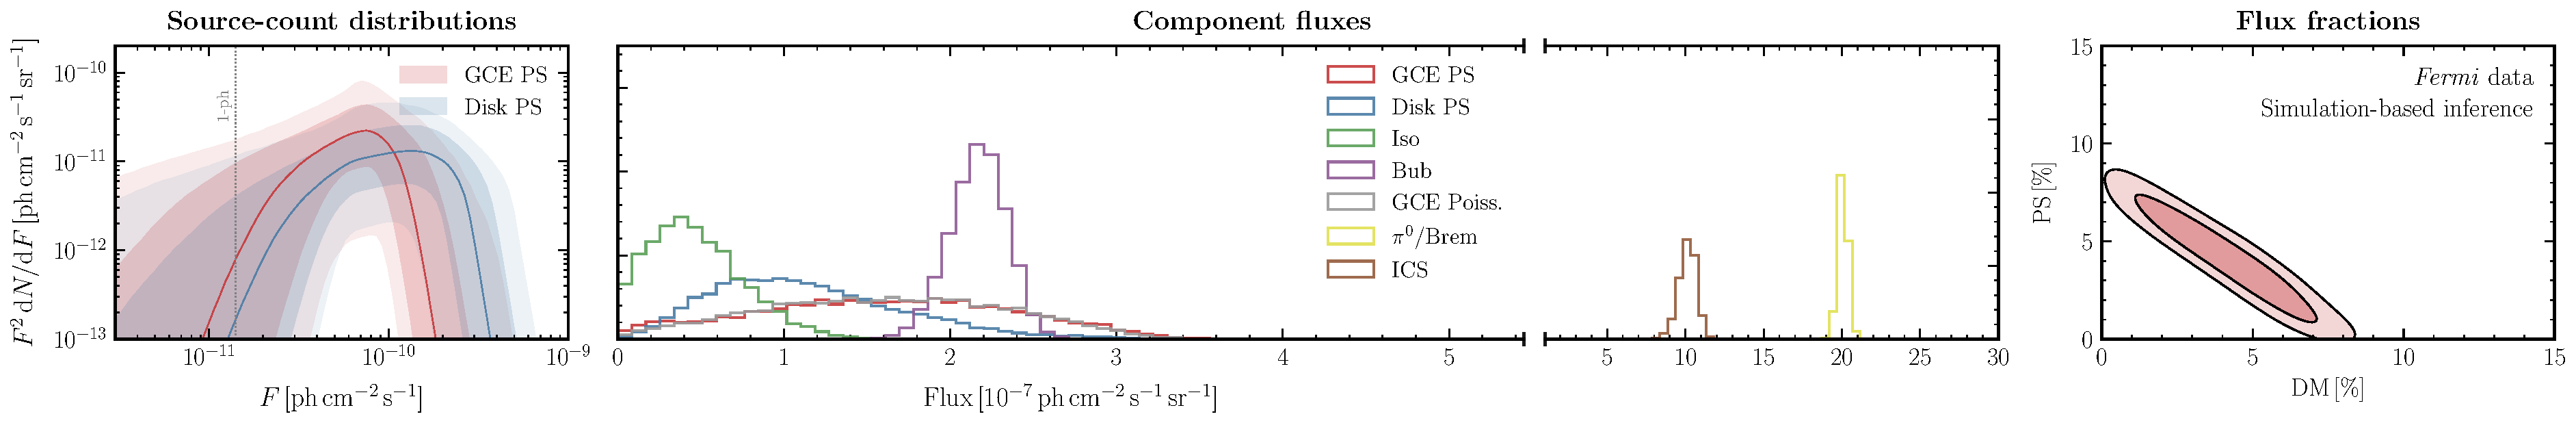
\includegraphics[width=0.95\textwidth]{plots/data_fid_sbi_thick.pdf}
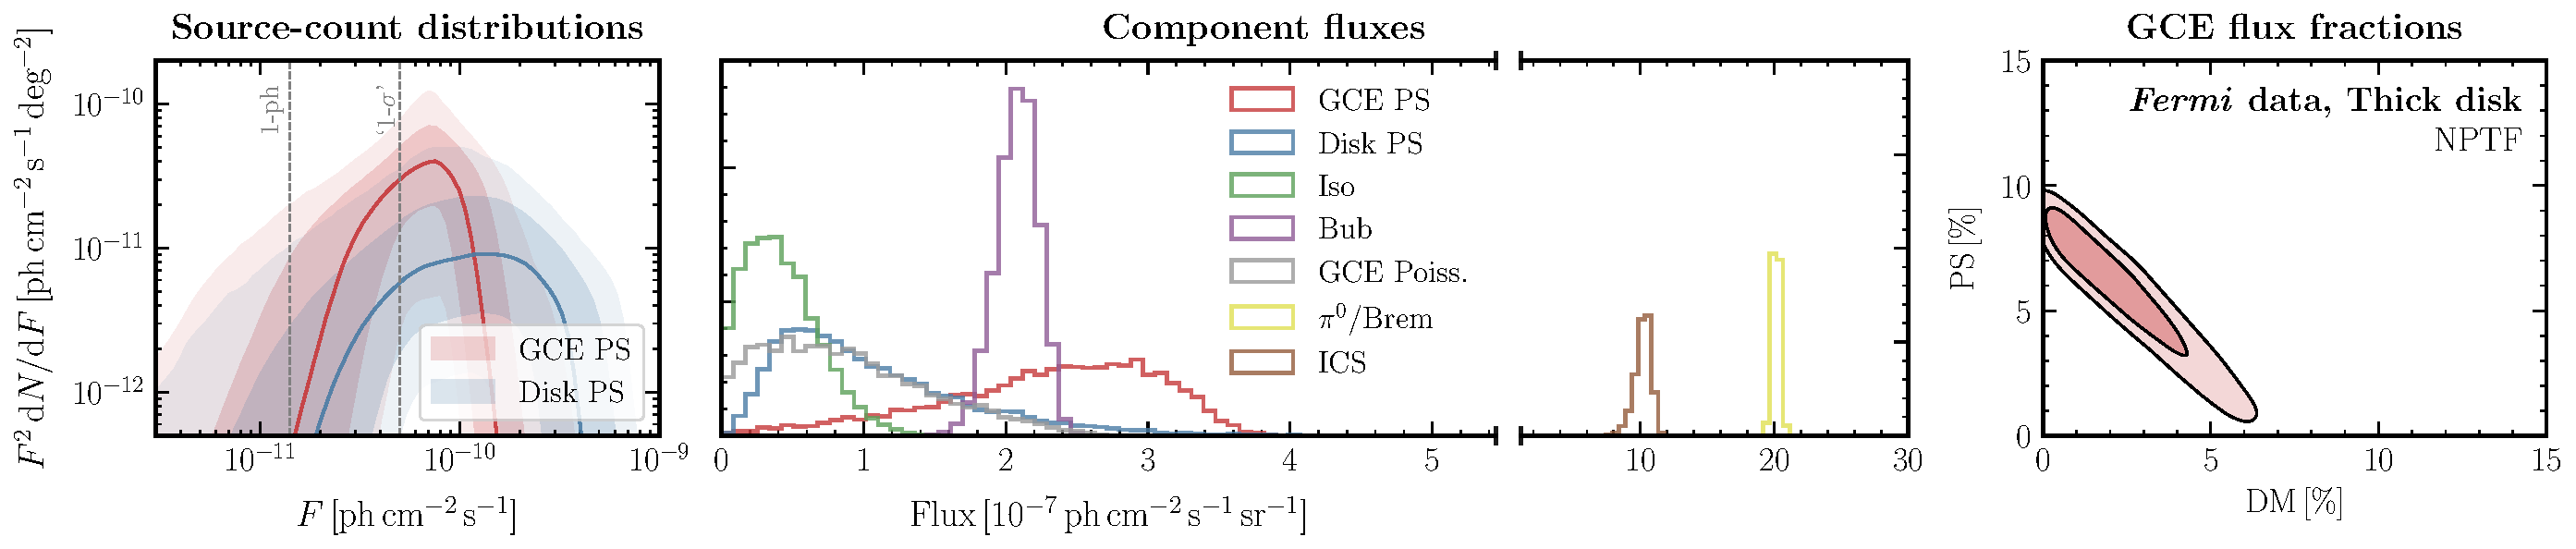
\includegraphics[width=0.95\textwidth]{plots/data_fid_nptf_thick.pdf}
\caption{Same as Fig.~\ref{fig:fid_data}, but for a model where the spatial distribution of disk-correlated PSs is modeled using a thick-disk template (scale factor $z_\mathrm{s}=1\,\mathrm{kpc}$ in Eq.~\eqref{eq:disk_spatial}) rather than the default thin-disk template ($z_\mathrm{s}=0.3\,\mathrm{kpc}$).}
\label{fig:fid_data_thick_disk}
\end{figure*}
%

We test the robustness of our results by exploring several systematic variations on the baseline analysis, using alternative descriptions for the diffuse foreground emission template and the spatial distribution of disk-correlated sources. Here, the neural network is re-trained on a new set of simulations obtained using the alternative forward model before applying it to \Fermi data. Results of these analysis variations are summarized in Tab.~\ref{tab:results}. \\

\noindent
\textbf{Variation on the diffuse foreground model:}
In addition to diffuse Model O considered in the baseline analysis, we consider the alternative Models A and F from Ref.~\cite{Calore:2014xka} to model the diffuse foreground emission, again including separate templates for gas-correlated emission and inverse Compton scattering. While shown to be a worse fit to the present dataset~\cite{Buschmann:2020adf}, these models have been previously used in the GCE literature~\cite{Buschmann:2020adf,Leane:2020pfc,Leane:2020nmi} and provide a useful comparison point.

Results for these variations are shown in Figs.~\ref{fig:fid_data_modelA} and~\ref{fig:fid_data_modelF}, respectively. In each case, results using the SBI pipeline are shown in the top row, with corresponding results using the NPTF pipeline in the bottom row. 
Qualitatively similar results are obtained when using Model A (Fig.~\ref{fig:fid_data_modelA}) compared to the baseline analysis in Fig.~\ref{fig:fid_data} using Model O, with $34.7^{+9.9}_{-19.8}\%$ of the GCE flux attributed to PS, roughly half the fraction found by the NPTF analysis. Using Model F on the other hand, $52.9^{+10.8}_{-26.1}\%$ of the emission is attributed to PSs, with a marginally larger amount found by the NPTF analysis. The total emission absorbed by the GCE in this case is about half of that found in the baseline scenario. This is consistent with the results of Ref.~\cite{Buschmann:2020adf}, which found that the total GCE flux could vary by up to a factor of $\sim 2$ between analyses using different diffuse models. \\

\noindent
\textbf{Variation on the disk template:}
The baseline scenario considered a disk-correlated PS population with a spatial distribution given by Eq.~\eqref{eq:disk_spatial}, setting the scale height scale height $z_\mathrm{s} = 0.3\,\mathrm{kpc}$ corresponding to the `thin-disk' scenario. Given uncertainties in the spatial distribution of the point source population (in particular, that of millisecond pulsars) associated with the Galactic disk, a `thick-disk' spatial distribution has been employed in the literature as an alternative model~\cite{Lee:2015fea,Leane:2019xiy,Buschmann:2020adf}, where the scale height is typically set to $z_\mathrm{s} = 1\,\mathrm{kpc}$. 

Results using a thick-disk template for the disk-correlated PS population are shown in Fig.~\ref{fig:fid_data_thick_disk}. For the SBI analysis, a larger fraction $51.5^{+9.2}_{-22.2}\%$ of the GCE flux is attributed to a PS population in this case compared to the baseline scenario, with the GCE flux itself being slightly larger. Once again, the NPTF analysis estimates a higher relative fraction $75.0^{+7.1}_{-22.6}\%$ of the GCE in point sources.\\

% \noindent
% \textbf{Variation of the ROI size:}
% Although the GCE signal is concentrated predominantly in the inner $10^\circ$, the use of the larger $25^\circ$ ROI in this work is motivated by the fact that a larger region may better constrain various spatially-extended modeled emission components. On the other hand, there is also the potential for more susceptibility to mismodeling effects when using a larger ROI. The right panel of Fig.~\ref{fig:variations} shows analysis results using smaller ROI sizes---$10^\circ, 15^\circ$ and $20^\circ$. These are seen to be completely consistent with the baseline analysis in the $25^\circ$ ROI, with a wider posterior in the smaller ROIs as expected since these contain less information than baseline ROI.

\section{Susceptibility to model misspecification}
\label{sec:mismodeling}

Given the complex astrophysical environment in the Galactic Center, a key challenge in $\gamma$-ray analyses of the GCE is that associated with effects of mismodeled signal and background templates. As explored in detail in Refs.~\cite{Lee:2015fea,Leane:2020pfc,Leane:2020nmi,Buschmann:2020adf,Chang:2019ars} within the NPTF framework, mismodeling can hamper the characterization of an Inner Galaxy PS population and, if sufficiently severe, can result in the attribution of mismodeled residuals to a spurious PS population when the underlying emission is actually smooth in nature. 

In this section we assess the susceptibility of our simulation-based inference pipeline to this scenario. We do so by creating mock data with a smooth GCE signal and a background model that was perturbed compared to the model that was used to train the SBI pipeline, and analyzing it with our baseline neural network \emph{i.e.}, the one trained on the forward model described in Sec.~\ref{sec:datasets} and used in the baseline analysis on data in Sec.~\ref{sec:data}. The ability of our method to correctly characterize the injected signal is then indicative of the level of robustness that can be expected in the real data under corresponding circumstances. Results for the various tests performed are shown in Fig.~\ref{fig:sim_sbi_mismo}, and will be described below. In each case, we show posteriors by combining samples obtained by analyzing 10 different mock datasets in order to characterize the `average' mismodeling associated with a given configuration. The first row of Fig.~\ref{fig:sim_sbi_mismo} shows the aggregate analysis without mismodeling \emph{i.e.}, using mock data created with the same same templates used for training the neural posterior and for inference, as a point of comparison. In all cases tested, while posteriors for certain templates can show systematic biases, preference for a smooth GCE remains robust and the fraction of PS-like emission is compatible with zero, as seen from the right-most column of Fig.~\ref{fig:sim_sbi_mismo}. \\

\noindent
\textbf{Test of diffuse mismodeling using an alternative template:}
We create mock data using diffuse Model A, and analyze it using our baseline analysis pipeline trained with Model O. The aggregated results over 10 different maps are shown in the second row of Fig.~\ref{fig:sim_sbi_mismo}. We see that while the marginalized DM posterior faithfully corresponds to the true underlying value, the PS template picks up small amount of residual flux. \\

\noindent
\textbf{A data-driven test of large-scale mismodeling:}
We construct a data-driven model of foreground mismodeling on large spatial scales (specifically, well above the scale of the instrumental PSF) and assess the ability of our method to recover a smooth DM-like signal in this case. Following Ref.~\cite{Mishra-Sharma:2020kjb}, we perform a Poissonian template analysis on the \Fermi dataset $x$, modulating the diffuse model template $T_{\mathrm{dif}}$, which describes the bremsstrahlung and neutral pion decay components of diffuse Model O, by an (exponentiated) Gaussian process (GP) $f$:
\begin{equation}
x \sim \operatorname{Pois}\left(\sum_{i \neq \mathrm{dif}} A_{i} T_{i}+\exp \left(f\right) A_{\mathrm{dif}} T_{\mathrm{dif}}\right).
\end{equation}
The other Poissonian templates $T_{i}$, including a GCE DM template and the inverse Compton component of the diffuse foreground model, are treated as before using an overall normalization factor $A_{i}$. $f \sim \mathcal{N}(m, K)$ is the GP component with prior mean $m$ set to zero, and the covariance $K$ described using the Mat\'ern kernel with smoothness parameter $\nu = 5/2$. We refer to Ref.~\cite{Mishra-Sharma:2020kjb} for further details of the analysis, as well a validation of the GP-augmented template fitting pipeline on simulated data.

Five random samples from the Gaussian process describing multiplicative mismodeling relative to the real \Fermi data when using our baseline diffuse Model O are shown in Fig.~\ref{fig:dd_mismo_map}. The largest mismodeling by magnitude in this case is inferred to be concentrated in the southern regions of the baseline ROI. We note that the recovered GCE flux tends to be lower by up to 40\% when using the GP-modulated diffuse model compared to that obtain in a Poissonian fit, indicating that a component of the centrally concentrated emission could be better described by the modulated template rather than the generalized NFW template modeling DM annihilation. We leave a detailed study of implications of this fact for the morphology of the excess to future work.

In order to test the effect of such mismodeling on recovery of a DM signal we modulate the bremsstrahlung and neutral pion decay-tracing components of Model O using samples drawn from the inferred Gaussian process. These simulated samples are used as mock data that are then analyzed with our baseline pipeline, where the unmodulated Model O was used to create training samples.

The results of this test are shown in the third row of Fig.~\ref{fig:sim_sbi_mismo}. It can be seen that while large-scale mismodeling can distort the total flux attributed to individual modeled components, preference for a smooth origin of the signal remains robust. \\

% %
% \begin{figure*}
%     \centering
%     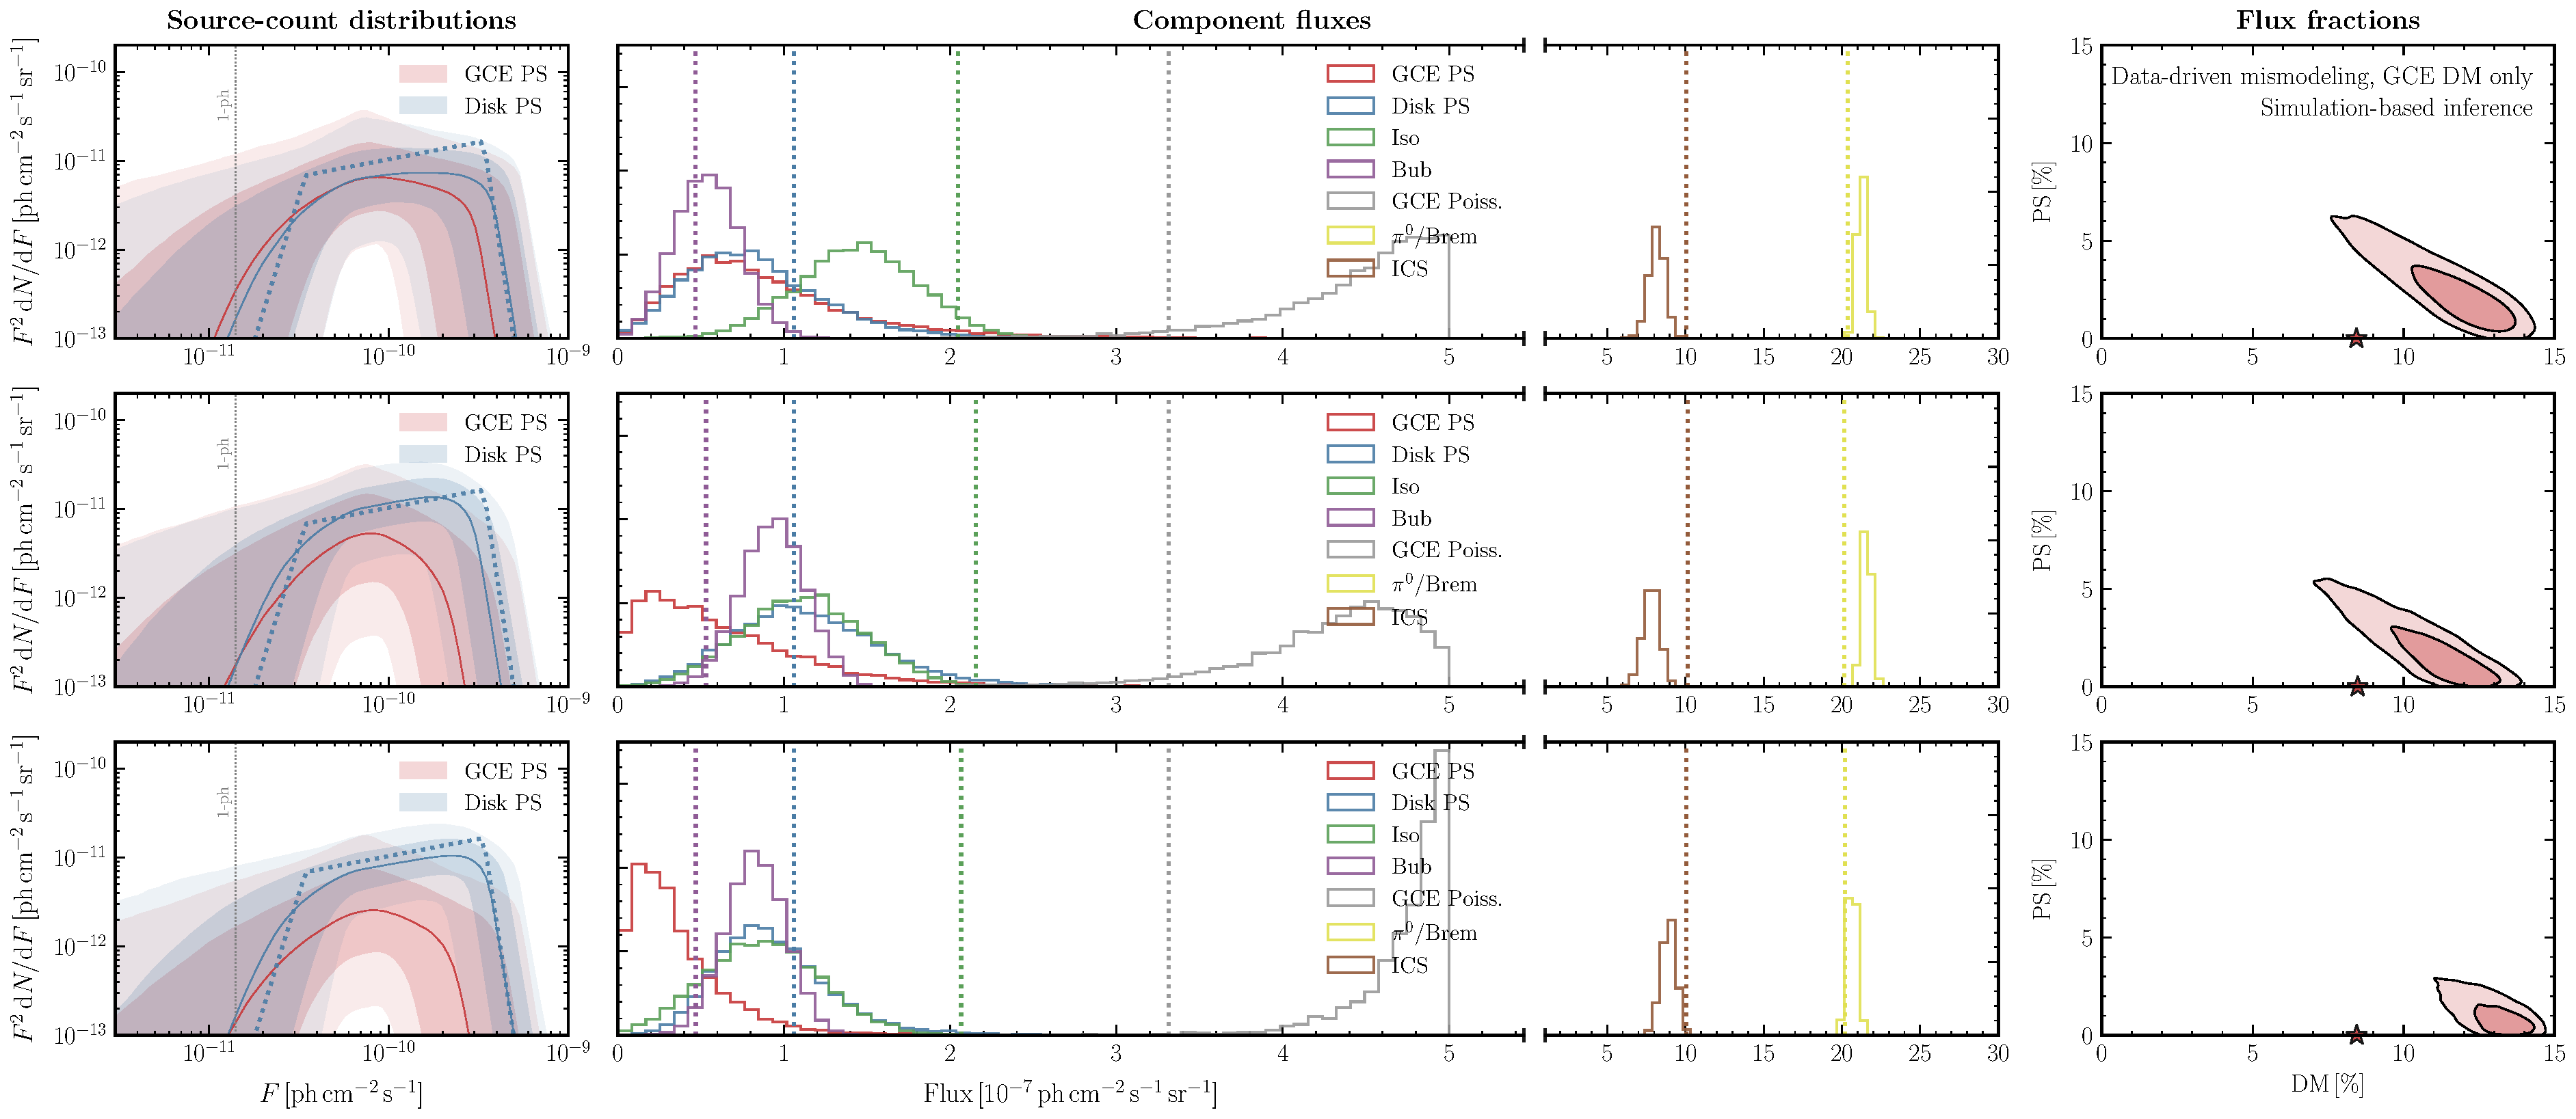
\includegraphics[width=0.95\textwidth]{plots/sim_sbi_dm_mismo.pdf}
%     \caption{Same as Fig.~\ref{fig:sim_sbi_dm}, but for simulated data where the GCE consists of purely DM-like emission and the diffuse model is modulated by draws from the Gaussian process description of diffuse mismodeling. DM-like emission is inferred in each case, although the magnitude of emission is overestimated as some of the diffuse mismodeling is absorbed into the Poissonian GCE component.}
%     \label{fig:sim_sbi_dm_mismo}
% \end{figure*}
% %

%
\begin{figure*}
\centering
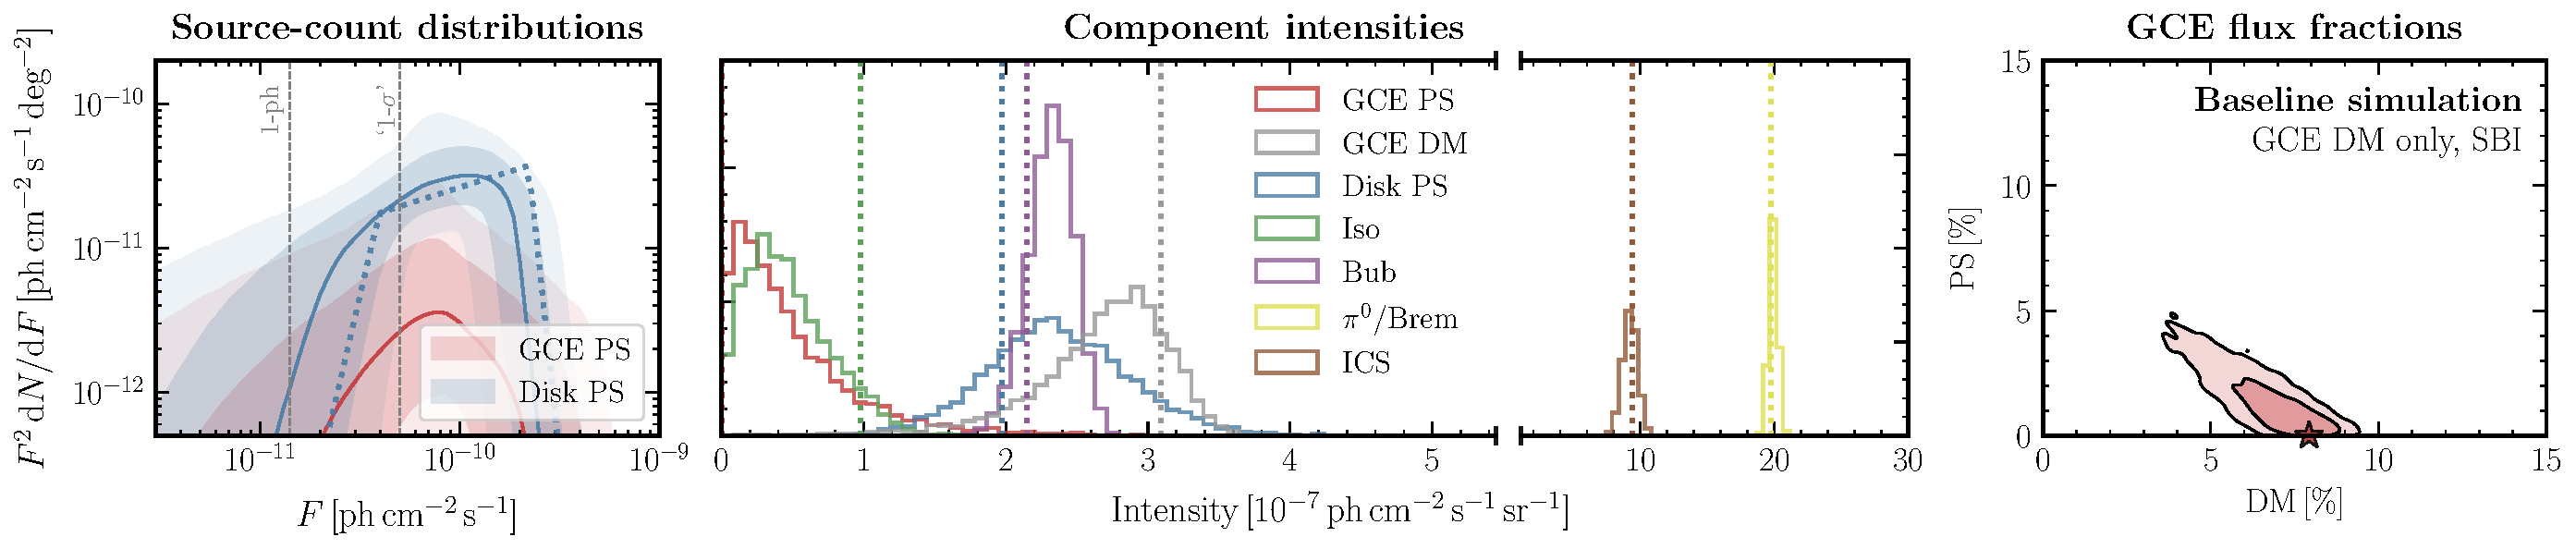
\includegraphics[width=0.95\textwidth]{plots/sim_sbi_dm_agg.pdf}
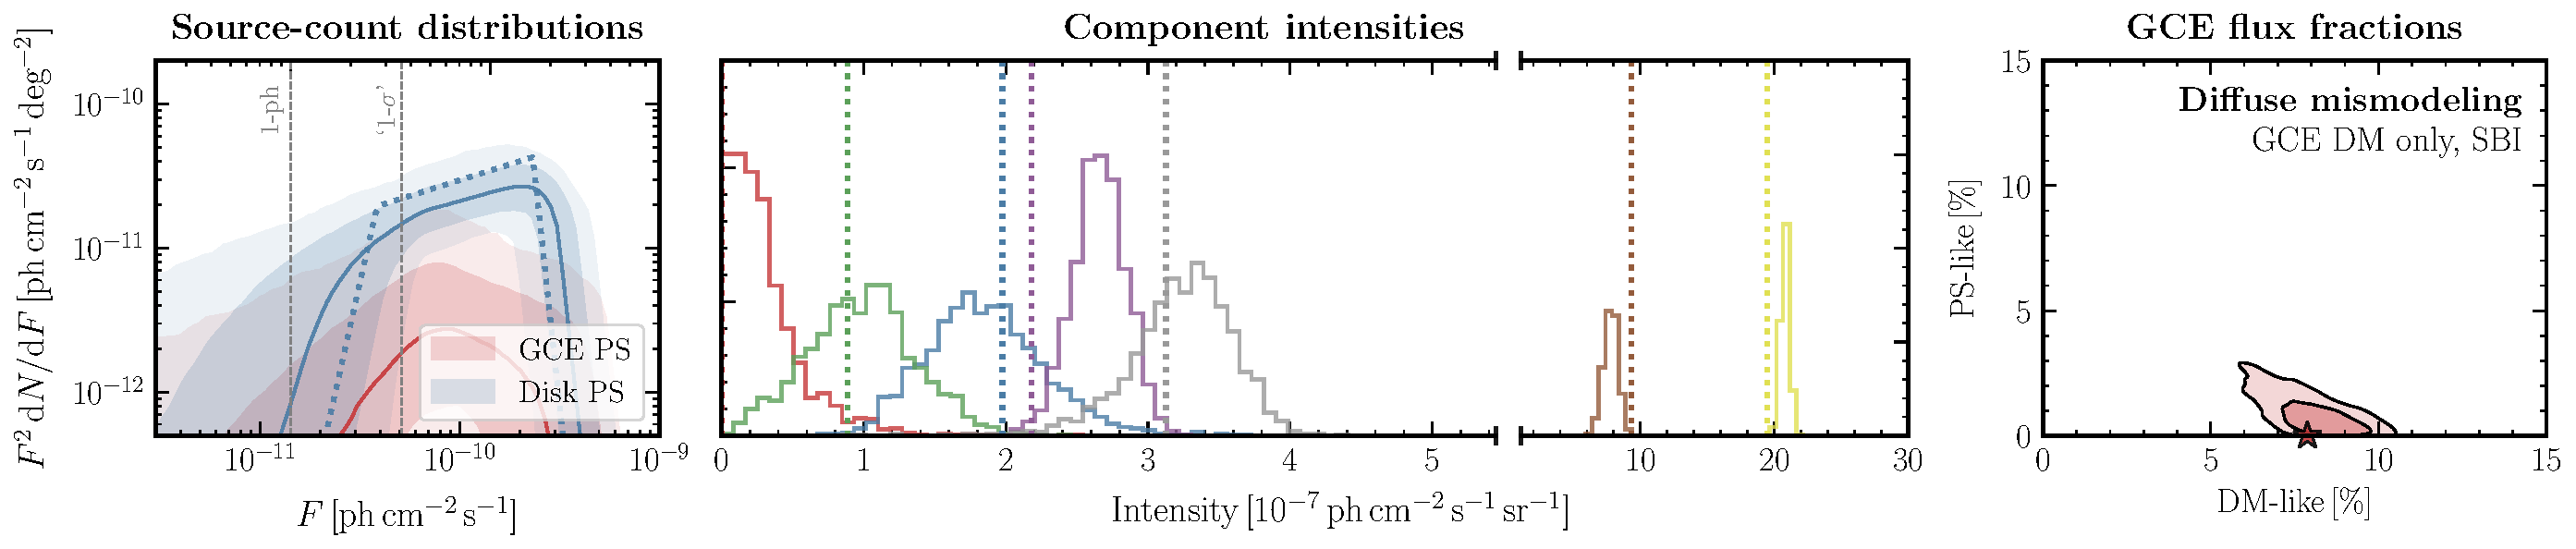
\includegraphics[width=0.95\textwidth]{plots/sim_sbi_modelA_dm.pdf}
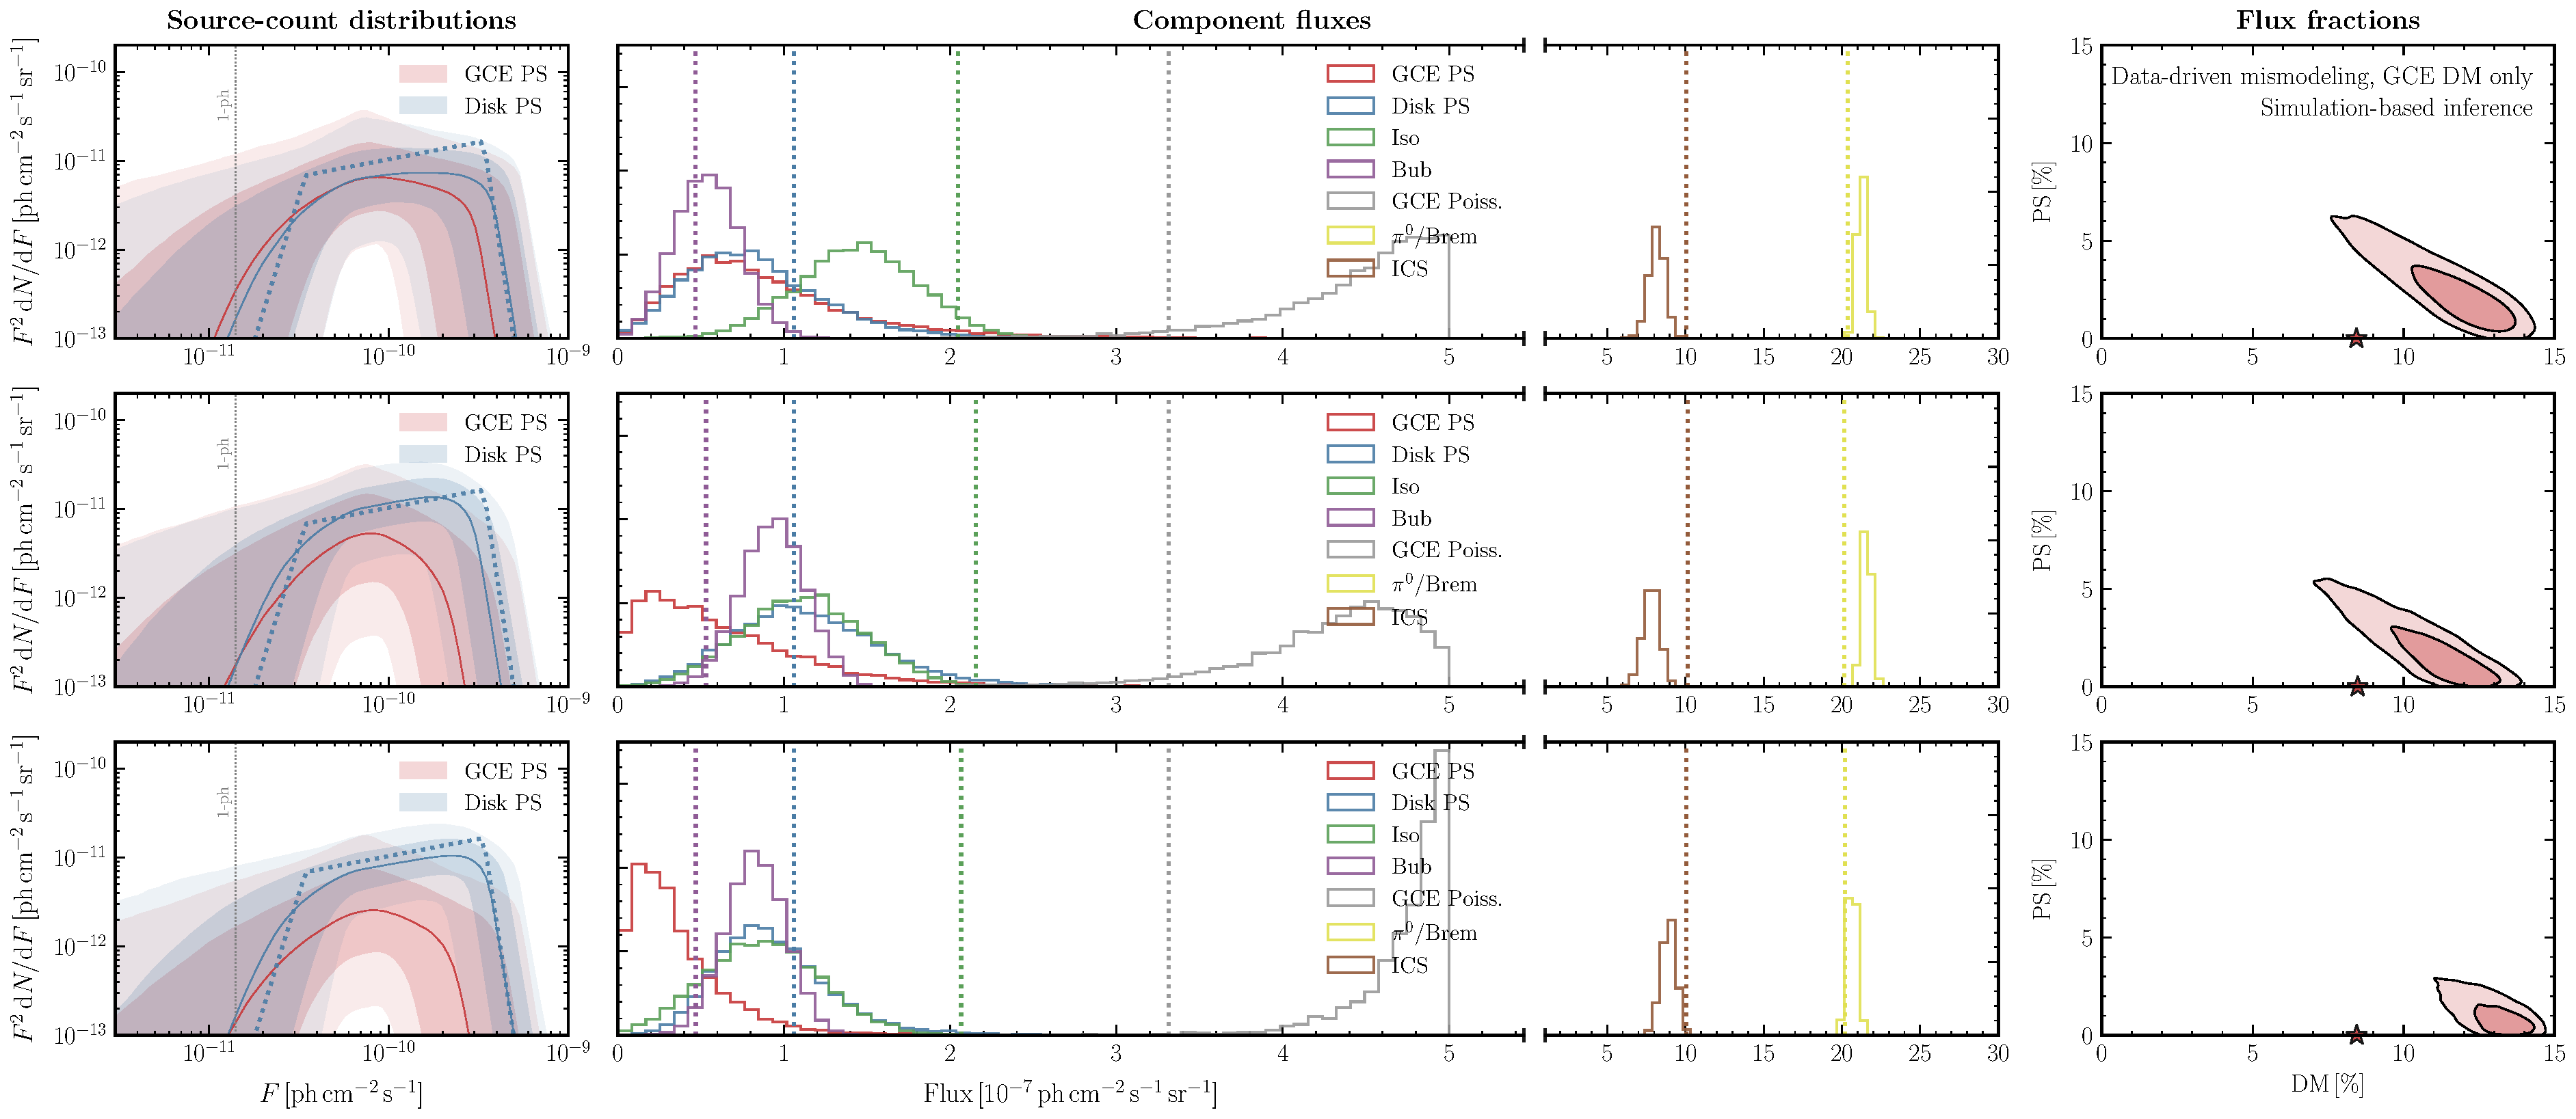
\includegraphics[width=0.95\textwidth]{plots/sim_sbi_dm_mismo.pdf}
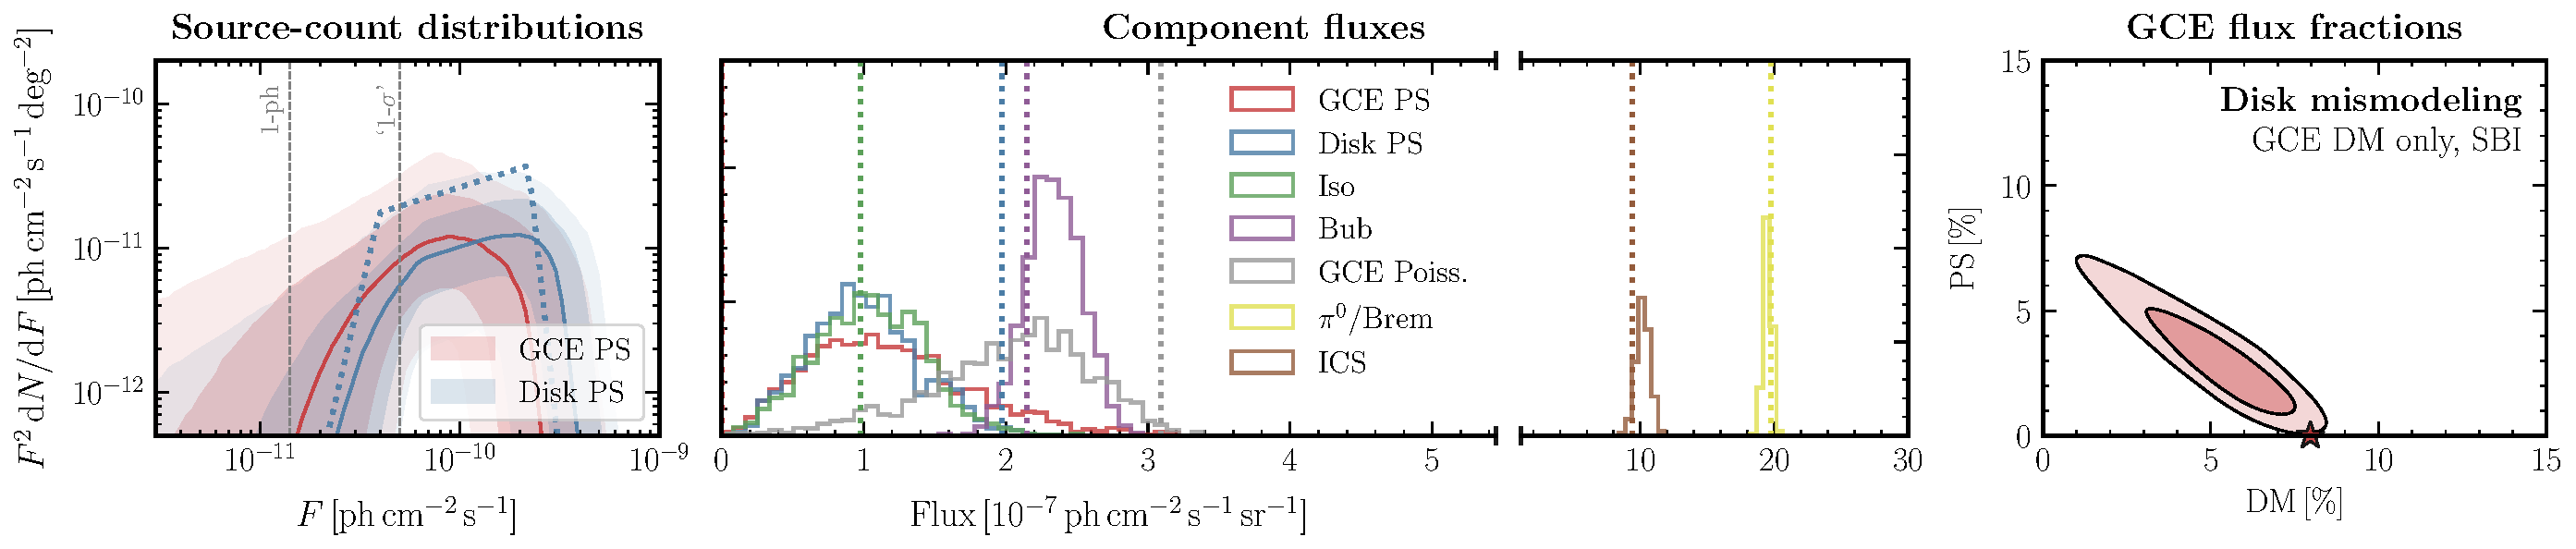
\includegraphics[width=0.95\textwidth]{plots/sim_sbi_thick_disk_mm_dm.pdf}
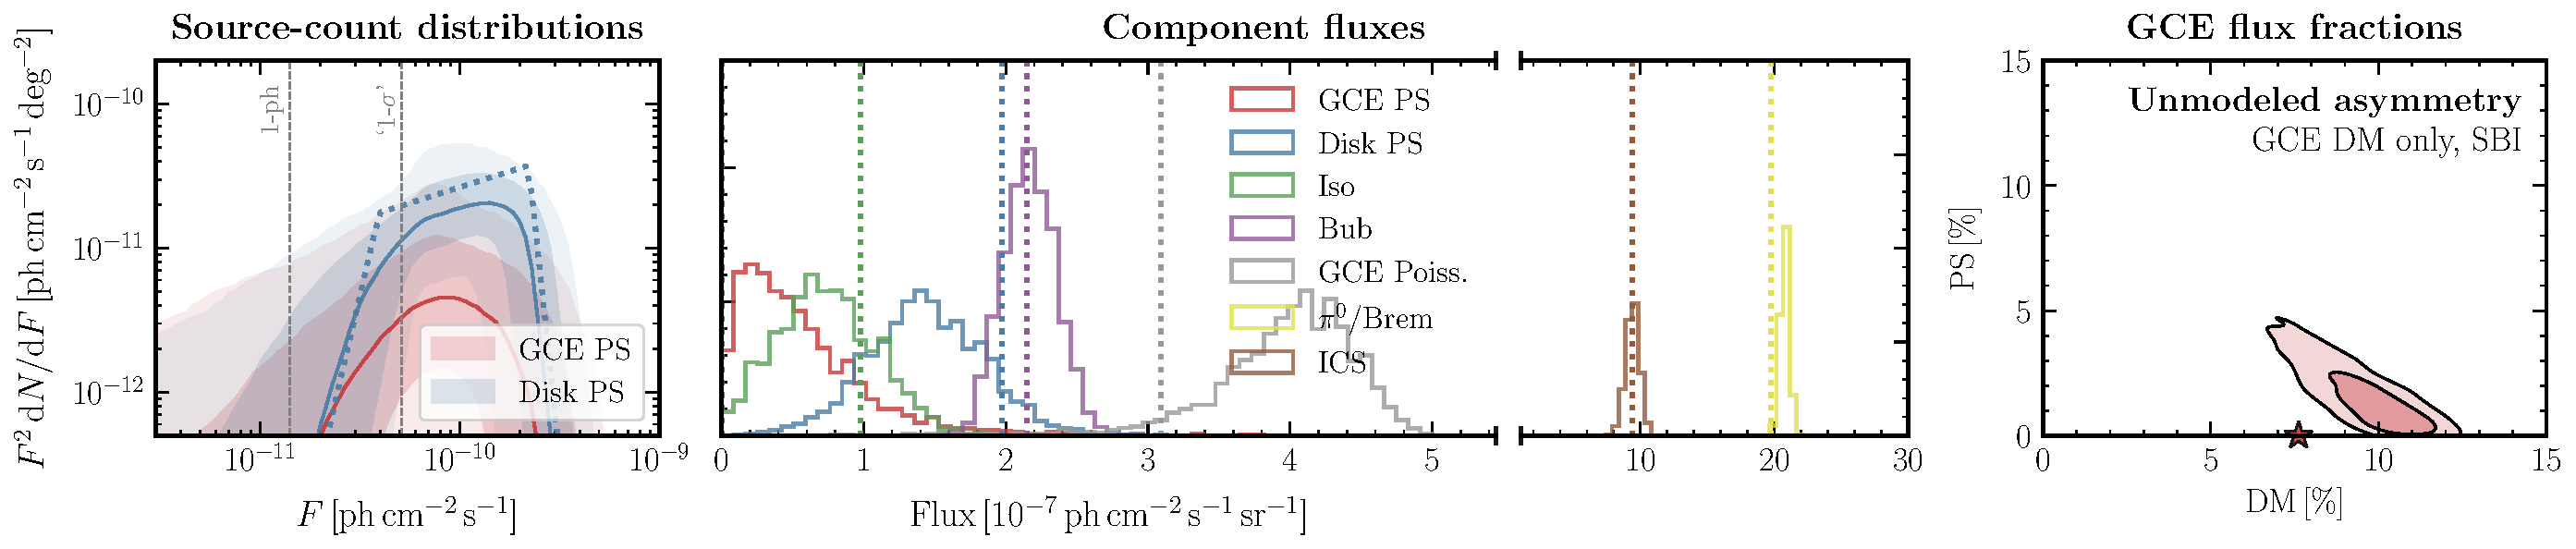
\includegraphics[width=0.95\textwidth]{plots/sim_sbi_dm_asym.pdf}
\caption{Effect of mismodeling on a smooth GCE within our analysis framework. Each row shows aggregate posteriors collected over 10 simulated samples; row-wise from top to bottom: \emph{(i)} No mismodeling; simulated data is constructed with the same templates as those used in the forward model. \emph{(ii)} Mock data created with diffuse Model A, showing the effect of diffuse mismodeling. \emph{(iii)} Mock data where the diffuse template, described by Model O, is modulated by draws from a Gaussian process modeling large-scale mismodeling inferred from the real \Fermi data. \emph{(iv)} Mock data where the thick-disk template is used in lieu of the thin-disk template. \emph{(v)} Mock data where the GCE signal in the Northern hemisphere is twice as large as that in the Southern hemisphere. While some PS-like emission is inferred, it is consistent with zero in all cases, and evidence for a smooth GCE is robust.}
\label{fig:sim_sbi_mismo}
\end{figure*}
%

\noindent
\textbf{Effect of mismodeling the disk spatial template:} 
We replace the thin-disk template, described by a scale height $z_\mathrm{s} = 0.3\,\mathrm{kpc}$ in Eq.~\eqref{eq:disk_spatial}, with a thick-disk template with $z_\mathrm{s} = 1\,\mathrm{kpc}$ in the simulated data. Results of then analyzing 10 mock maps using the thin-disk template used in the baseline configuration are shown in the fourth row of Fig.~\ref{fig:sim_sbi_mismo}. While disk mismodeling can distort the inferred SCD of disk-correlated PSs away from the truth, the smooth GCE signal is seen to be successfully recovered in this case. \\

%
\begin{figure*}
    \centering
    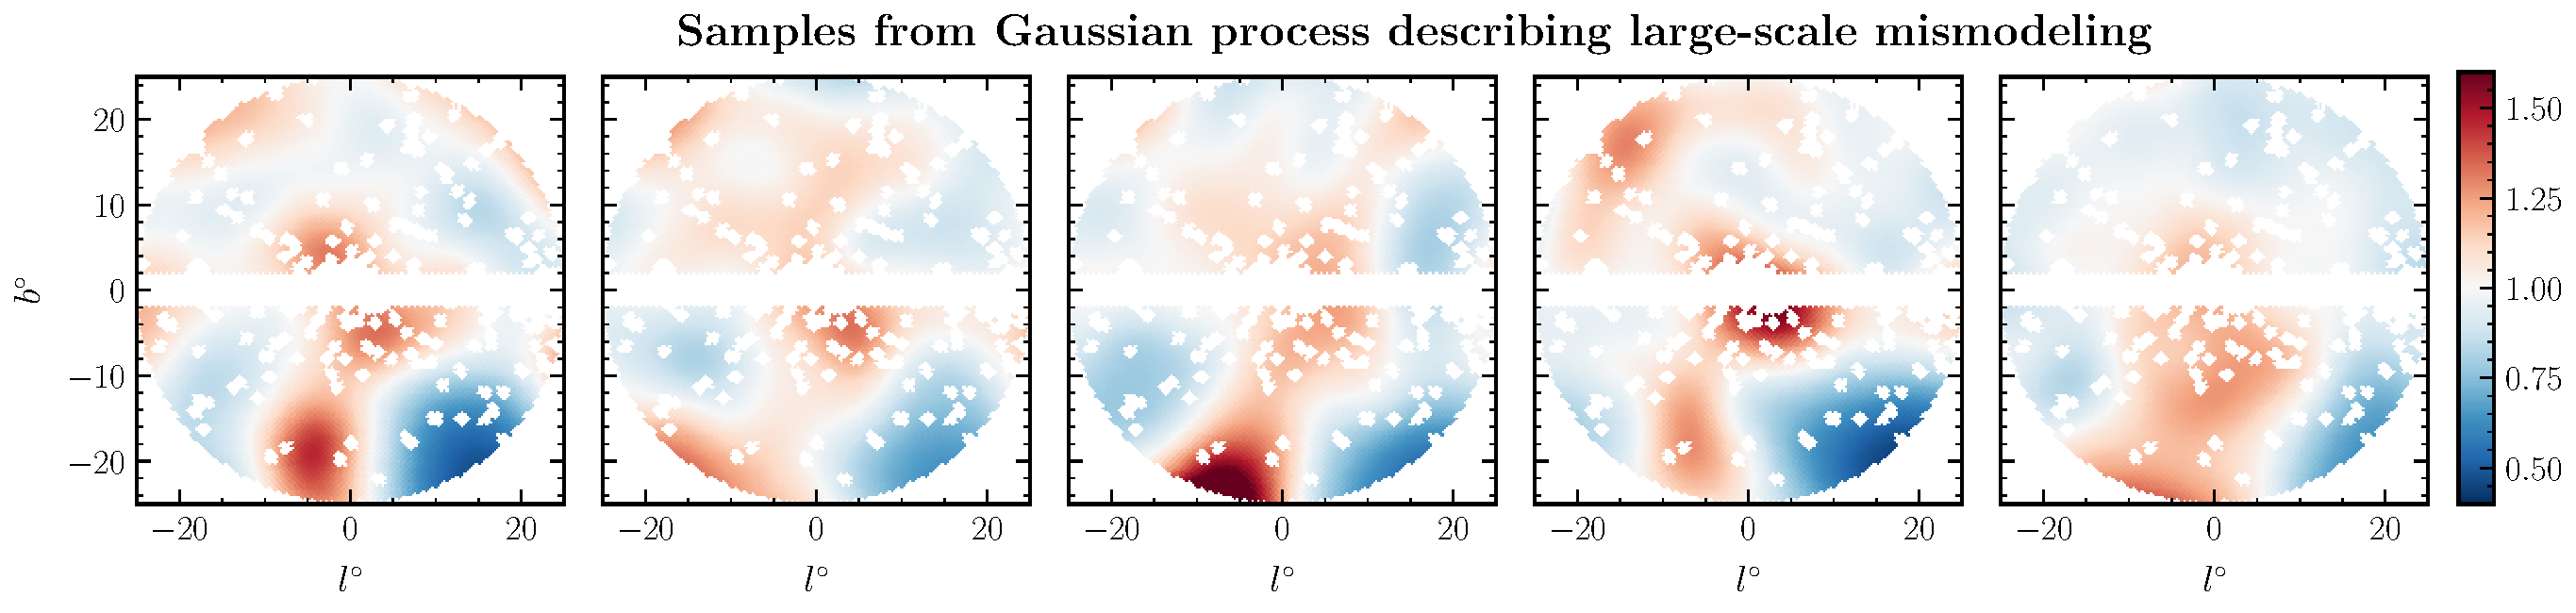
\includegraphics[width=0.95\textwidth]{plots/dd_mismo_map.pdf}
    \caption{Five random samples from the Gaussian process description of large-scale multiplicative mismodeling associated with the gas-correlated component of diffuse foreground Model O when applied to the real \Fermi data.}
    \label{fig:dd_mismo_map}
    \end{figure*}
    %

\noindent
\textbf{Effect of an unmodeled asymmetry in the signal:}
Besides mismodeling associated with astrophysical background templates, another concern is that associated with mismodeling of the signal emission itself. In particular, as pointed out in Refs.~\cite{Leane:2020nmi,Leane:2020pfc}, a North-South asymmetry in a putative dark matter signal, if unaccounted for, could lead to spurious inference of a PS population associated with the purely smooth, asymmetric signal in the NPTF framework. Refs.~\cite{Leane:2020nmi,Leane:2020pfc} found preference for such a scenario in real \Fermi data, with the GCE signal in the Northern hemisphere a factor of $\sim2$ larger than that in the Southern hemisphere when the GCE template in the two regions is floated separately in a ROI defined by $r < 10^\circ$. In this case, for certain diffuse models, no preference for a PS-like GCE was found in contrast to the case when a single template was used to model the GCE. 

We test the impact of a North-South-asymmetric dark matter signal within our framework by running our baseline pipeline on simulated datasets where the dark matter-like signal in the Northern hemisphere of the ROI is 2 times larger than that in the Southern hemisphere, mimicking the preference in real data found in Refs.~\cite{Leane:2020nmi,Leane:2020pfc}. The results of this test on 10 such simulated realizations is shown in the last row of Fig.~\ref{fig:sim_sbi_mismo}. We see that the presence of a substantially asymmetric DM signal has only a marginal impact on the inferred posteriors, and does not lead to a spurious preference for a PS population as was found in the NPTF framework. We attribute this to the fact that the \texttt{DeepSphere}-based feature extractor can account for pixel-to-pixel correlations in the $\gamma$-ray counts map, and can thus be sensitive to \emph{local} PS-like structures. In contrast, the 1-point PDF-based NPTF framework, being agnostic to the ordering of the pixels, can notice spurious PS-like structures in the distribution of `residuals' associated with an asymmetric signal when analyzed with a symmetric template.
As done in Ref.~\cite{Buschmann:2020adf}, we emphasize that the presence of an asymmetry in the GCE signal, if not attributed to diffuse mismodeling, would point towards astrophysical explanations of the GCE since a true dark matter signal would not be expected to be significantly asymmetric.
    
% %
% \begin{figure*}
%     \centering
%     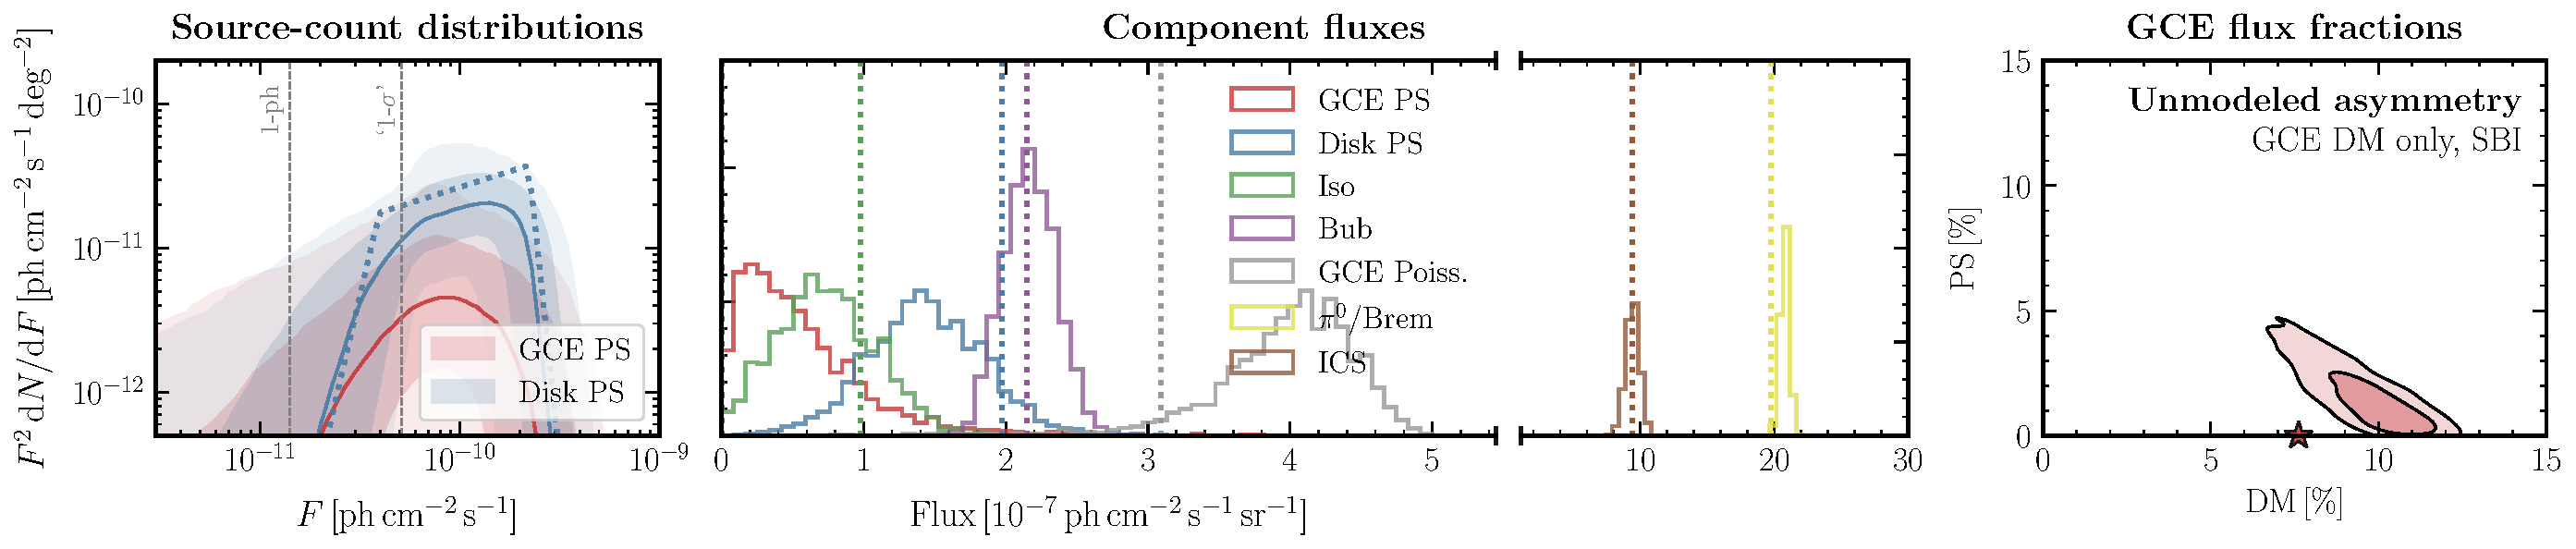
\includegraphics[width=0.95\textwidth]{plots/sim_sbi_dm_asym.pdf}
%     \caption{Same as Fig.~\ref{fig:sim_sbi_dm}, but for simulated data where the GCE consists of purely DM-like emission with a North-South asymmetry; the signal in the Northern hemisphere is larger by a factor of 3. The mismodeled signal is seen to have marginal qualitative effect on the recovery of DM-like emission.}
%     \label{fig:sim_sbi_dm_asym}
% \end{figure*}
% %

\section{Discussion and conclusions}
\label{sec:conclusion}

In this paper, we have leveraged recent advances in neural simulation-based inference in order to jointly characterize a putative DM-like signal and PS population associated with the observed \Fermi Galactic Center Excess. Consistent with Ref.~\cite{List:2020mzd} which used a Bayesian neural network and first leveraged a \texttt{DeepSphere}-based feature extraction architecture for analyzing $\gamma$-ray data in the Galactic Center region, our analysis based on conditional posterior density estimation with normalizing flows finds a reduced contribution associated with a potential population of unresolved PSs to the GCE compared to previous analyses based on the photon statistics of the $\gamma$-ray map. In particular, depending on the analysis configuration, we find a median value of $\sim30$--$50\%$ as the fraction of GCE emission that can be attributed to a PS population, with the inferred source-count distribution peaking at smaller fluxes $\sim2$--$3\times 10^{-11}$\,ph\,cm$^{-2}$\,s$^{-1}$ compared to values found in previous analyses based on the non-Poissonian template fitting (NPTF) framework~\cite{Lee:2015fea}, where the SCD is seen to peak just below the threshold for resolution of individual PSs. The NPTF analyses performed in this work find a similarly dim source-count distribution, in all cases however attributing a larger fraction $\sim50$--$75\%$ of the GCE to a PS population as compared to the corresponding SBI analyses.

The results of this paper are broadly consistent with and complementary to those obtained in Ref.~\cite{List:2021aer}, which used a \texttt{DeepSphere}-based architecture which was, in contrast to our parametric approach, combined with a novel neural network-based approach to inferring the counts distributions associated to PS populations using histograms with modeled uncertainties~\cite{list2021earth}. Their approach does not explicitly distinguish between Poissonian and PS-like components, treating emission associated with the inferred counts PDF below some threshold as effectively Poissonian. While this makes a direct comparison to the results of their analysis challenging, the overall conclusions regarding the fraction of emission that can be attributed to PSs and the characteristics of the GCE and disk source-count distributions are qualitatively similar between the two studies. In particular, both papers find a dimmer GCE-correlated source-count distribution, with a smaller lower bound $\gtrsim \mathcal O(30\%)$ on the fraction of the total GCE emission associated to PSs compared to previous studies based on the NPTF.

Our qualitative conclusions are robust to the systematic variations we have explored, including different models for the diffuse foreground and spatial distribution of disk-correlated PS emission. We used a novel Gaussian process-based method to construct a data-driven model of large-scale spatial mismodeling, finding our method to be resilient to such effects when it comes to inferring the presence of a DM-like. As in any Galactic Center $\gamma$-ray analysis, we caution of the potential of unknown systematics, such as mismodeling on the scale of the size of the \Fermi-LAT point-spread function, to bias the results and conclusions of our analysis. Although machine learning-based analyses can utilize more of the information encoded in the forward model, and in particular in the present case can take advantage of pixel-to-pixel correlations, this can also make them more susceptible to specific modeled features compared to traditional techniques based on data reduction to hand-crafted data summaries. We leave a more detailed investigation of the impact of these effects to future work.

Several improvements to the framework presented here are possible. Although we have used a dataset restricted to the top quartile of photons by quality of PSF reconstruction, as shown in Ref.~\cite{Leane:2020pfc} the use of a larger data sample can provide improved sensitivity to a PS population while acting as a consistency check with results obtained on the smaller sample. The inclusion of energy-binning information in the analysis can be implemented in a straightforward manner by splitting up the data and template maps into individual energy bins and feeding these as separate channels in the graph-convolutional feature extraction network. The use of more complex feature extraction architectures can additionally improve the robustness of our results. 
While we have considered a simulated-based inference framework based on posterior density estimation with normalizing flows, alternative frameworks based on likelihood-ratio estimation~\cite{Brehmer:2018eca,Brehmer:2018hga,Brehmer:2018kdj,Cranmer:2015bka, Hermans:2019ioj,Miller:2020hua,Miller:2021hys} or flow-based likelihood estimation~\cite{winkler2019learning,papamakarios2019sequential} can provide complementary ways to characterize the $\gamma$-ray PS population in the Galactic Center. Additionally, the use of sequential active-learning methods~\cite{papamakarios2019sequential} and methods that make use of additional latent information from the simulator~\cite{Brehmer:2018eca,Brehmer:2018hga,Brehmer:2018kdj,Brehmer:2019xox,Stoye:2018ovl} can significantly improve the simulation sample efficiency and allow for extensions to more complex forward models, which can be important in particular for an energy-binned analysis and if including additional degrees of freedom for the astrophysical background models. 

Since diffuse mismodeling is the largest source of uncertainty in any analysis that aims to characterize the GCE, we also note the possibility of using adversarial learning methods~\cite{Louppe:2016ylz} or distance correlations~\cite{Kasieczka:2020yyl} to account for systematic differences between the modeled and real \Fermi data. Alternatively, generative modeling of the diffuse foreground either in a Gaussian process-based data-driven framework or using, \emph{e.g.}, autoencoders trained on an ensemble of plausible diffuse models, can provide a principled way to account for the large latent space associated with diffuse emission modeling. Motivated by quantitative variations in our results on \Fermi data when using different disk templates, self-consistently accounting for plausible variations in the spatial distribution of disk-correlated PSs can strengthen the results of our analysis when it comes to characterizing the PS population in the Galactic Center. 
These extensions can lead to a more robust characterization of an unresolved PS population in the Galactic Center region associated with the GCE, and we leave their study to future work.

The code used to obtain the results in this paper as well as the pre-trained neural network model associated with the baseline analysis is available at \url{https://github.com/smsharma/fermi-gce-flows}.

% \SM{Beef up attribution to previous papers on different topics.}

\vspace{.2cm}
%%%%%%%%%%%%%%%

\begin{acknowledgments}

We thank Johann Brehmer and Tracy Slatyer for helpful conversations. We are grateful to Florian List and Nick Rodd for carefully reading an earlier version of this paper and for their many helpful comments.
SM would like to thank the Center for Computational Astrophysics at the Flatiron Institute for their hospitality while this work was being performed. 
This work was performed in part at the Aspen Center for Physics, which is supported by National Science Foundation grant PHY-1607611.
The participation of SM at the Aspen Center for Physics was supported by the Simons Foundation.
SM is supported by the NSF CAREER grant PHY-1554858, NSF grants PHY-1620727 and PHY-1915409, and the Simons Foundation. 
KC is partially supported by NSF awards ACI-1450310, OAC-1836650, and OAC-1841471, the NSF grant PHY-1505463, and the Moore-Sloan Data Science Environment at NYU. 
This work is supported by the National Science Foundation under Cooperative Agreement PHY-2019786 (The NSF AI Institute for Artificial Intelligence and Fundamental Interactions, \url{http://iaifi.org/}).
This material is based upon work supported by the U.S. Department of Energy, Office of Science, Office of High Energy Physics of U.S. Department of Energy under grant Contract Number DE-SC0012567.
We thank the \Fermi-LAT Collaboration for making publicly available the $\gamma$-ray data used in this work.
This work made use of the NYU IT High Performance Computing resources, services, and staff expertise. 
This research has made use of NASA's Astrophysics Data System. 
This research made use of the \texttt{astropy}~\cite{Price-Whelan:2018hus,Robitaille:2013mpa}, \texttt{dynesty}~\cite{Speagle_2020}, \texttt{getdist}~\cite{Lewis:2019xzd}, \texttt{IPython}~\cite{PER-GRA:2007}, \texttt{Jupyter}~\cite{Kluyver2016JupyterN}, \texttt{matplotlib}~\cite{Hunter:2007}, \texttt{MLflow}~\cite{chen2020developments}, \texttt{nflows}~\cite{nflows}, \texttt{NPTFit}~\cite{Mishra-Sharma:2016gis}, \texttt{NumPy}~\cite{harris2020array}, \texttt{pandas}~\cite{pandas:2010}, \texttt{PyGSP}~\cite{michael_defferrard_2017_1003158}, \texttt{Pyro}~\cite{bingham2018pyro}, \texttt{PyTorch}~\cite{NEURIPS2019_9015}, \texttt{PyTorch Geometric}~\cite{Fey/Lenssen/2019}, \texttt{PyTorch Lightning}~\cite{william_falcon_2020_3828935}, \texttt{seaborn}~\cite{seaborn}, \texttt{sbi}~\cite{tejero-cantero2020sbi}, \texttt{scikit-learn}~\cite{scikit-learn}, \texttt{SciPy}~\cite{2020SciPy-NMeth}, and \texttt{tqdm}~\cite{da2019tqdm} software packages. We acknowledge the use of data products and templates from the code repository associated with Ref.~\cite{List:2020mzd}.\footnote{\url{https://github.com/FloList/GCE_NN}} 
We acknowledge the use of the code repository associated with Ref.~\cite{defferrard2020deepsphere}, in particular the implementation of the \texttt{DeepSphere} graph convolutional layer.\footnote{\url{https://github.com/deepsphere/deepsphere-pytorch}}
\end{acknowledgments}

\bibliographystyle{apsrev4-1}
\bibliography{fermi-gce-flows}

\appendix

%
\begin{figure*}
    \centering
    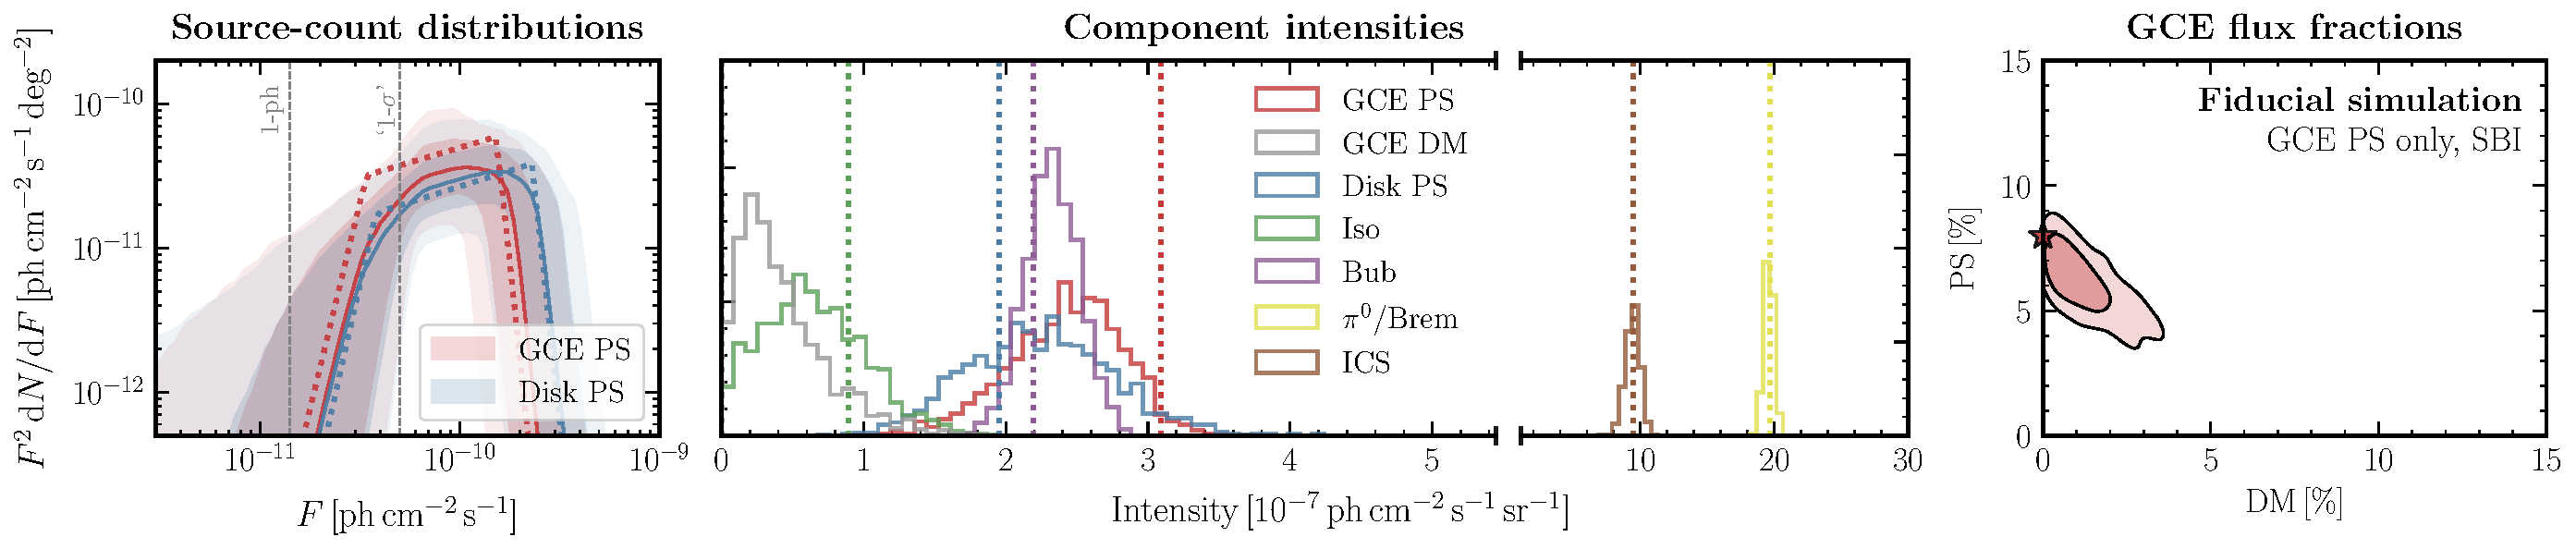
\includegraphics[width=0.95\textwidth]{plots/sim_sbi_ps_agg.pdf}
    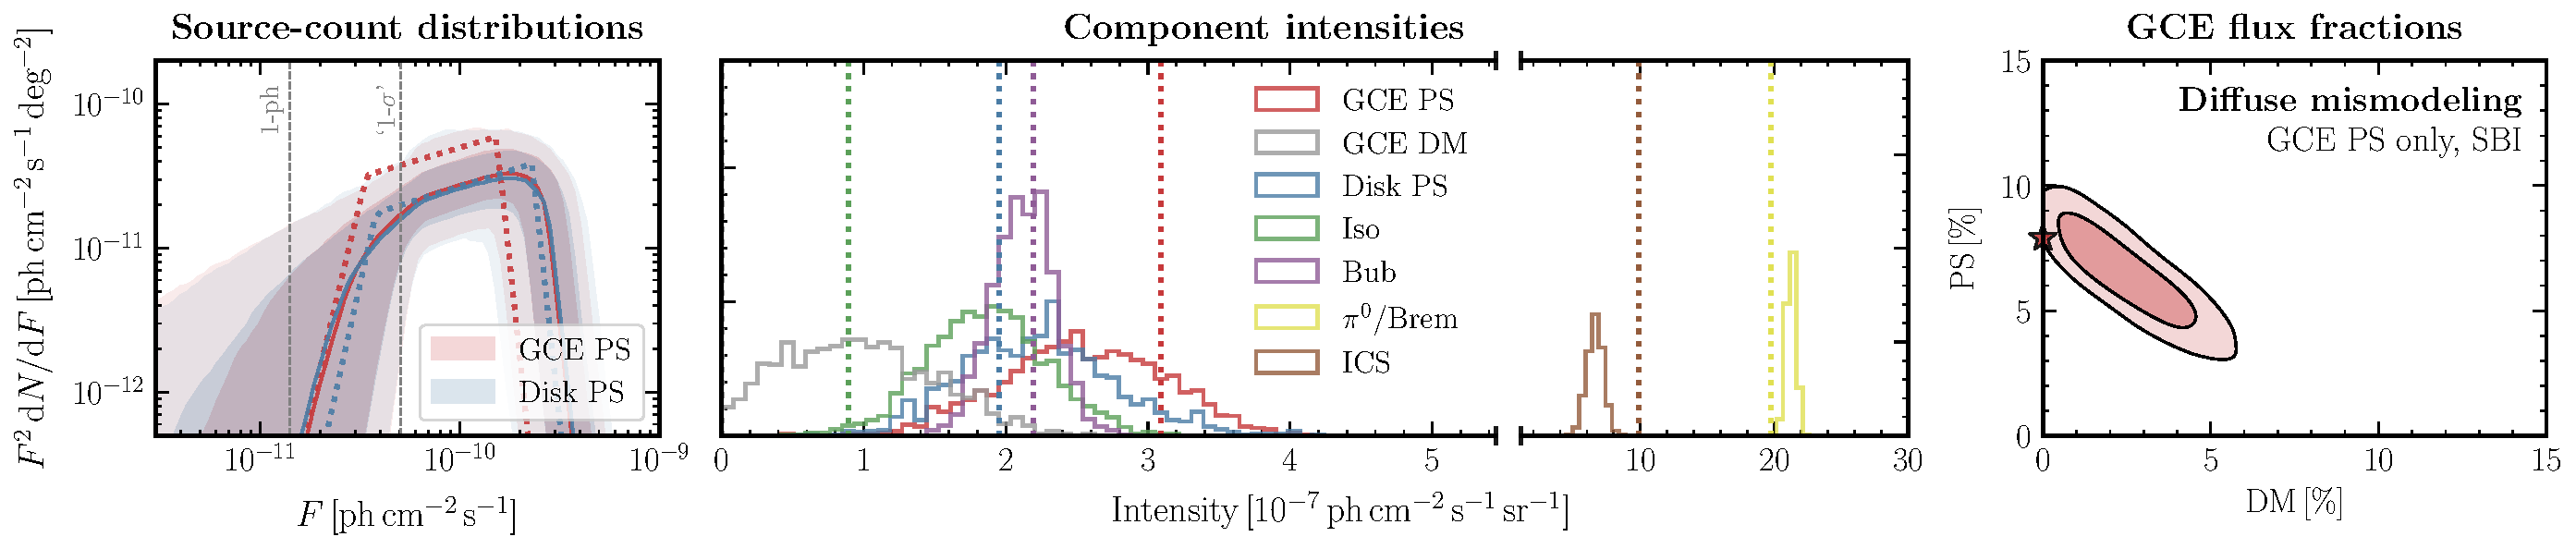
\includegraphics[width=0.95\textwidth]{plots/sim_sbi_modelA_ps.pdf}
    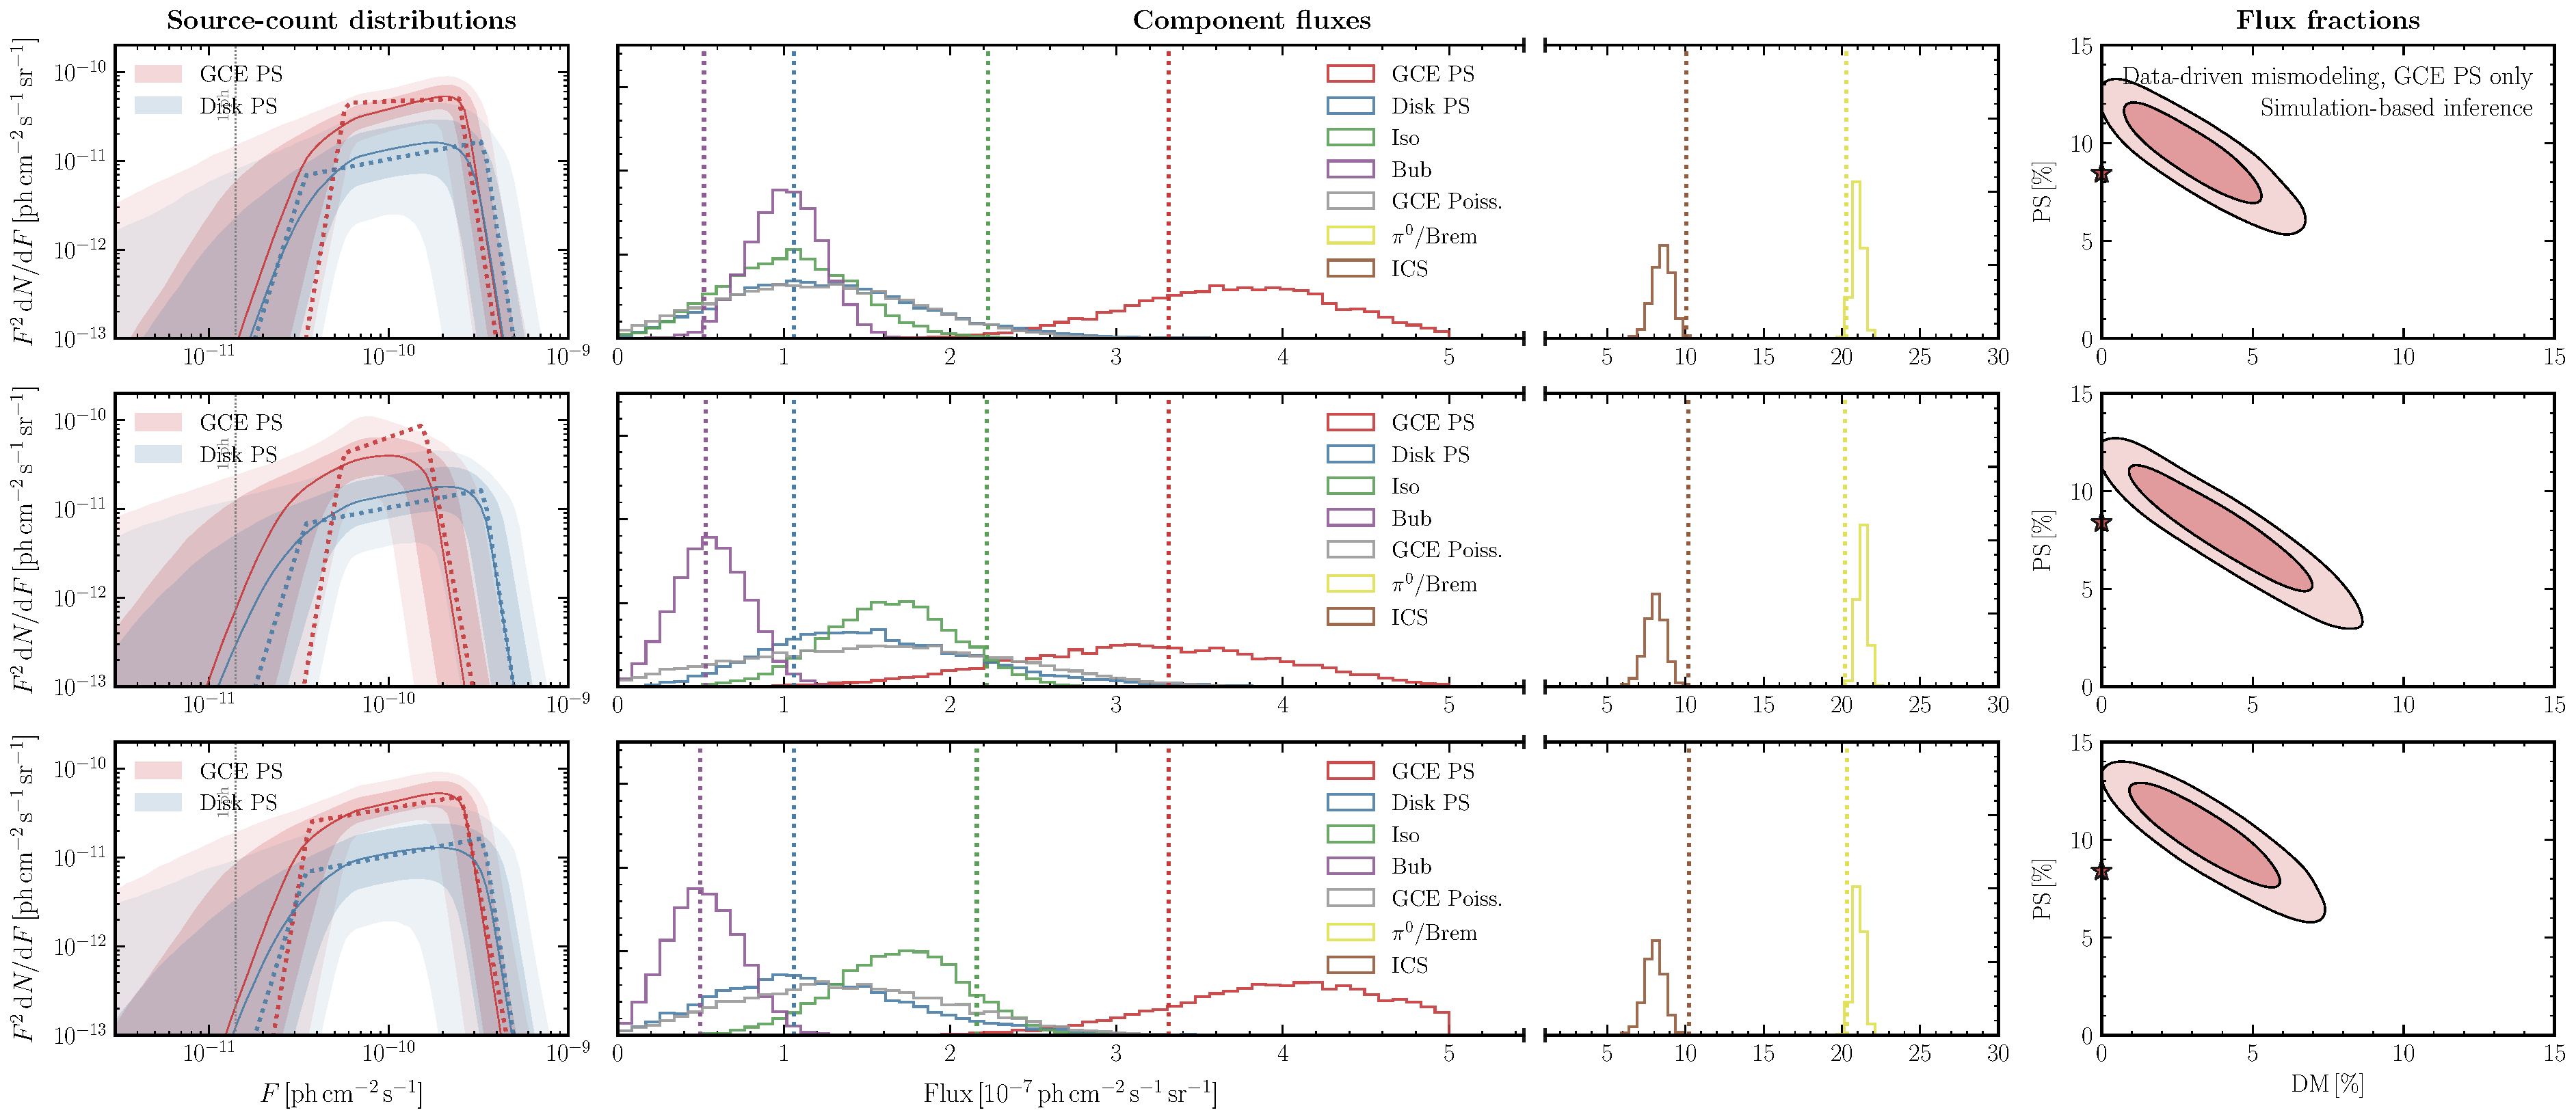
\includegraphics[width=0.95\textwidth]{plots/sim_sbi_ps_mismo.pdf}
    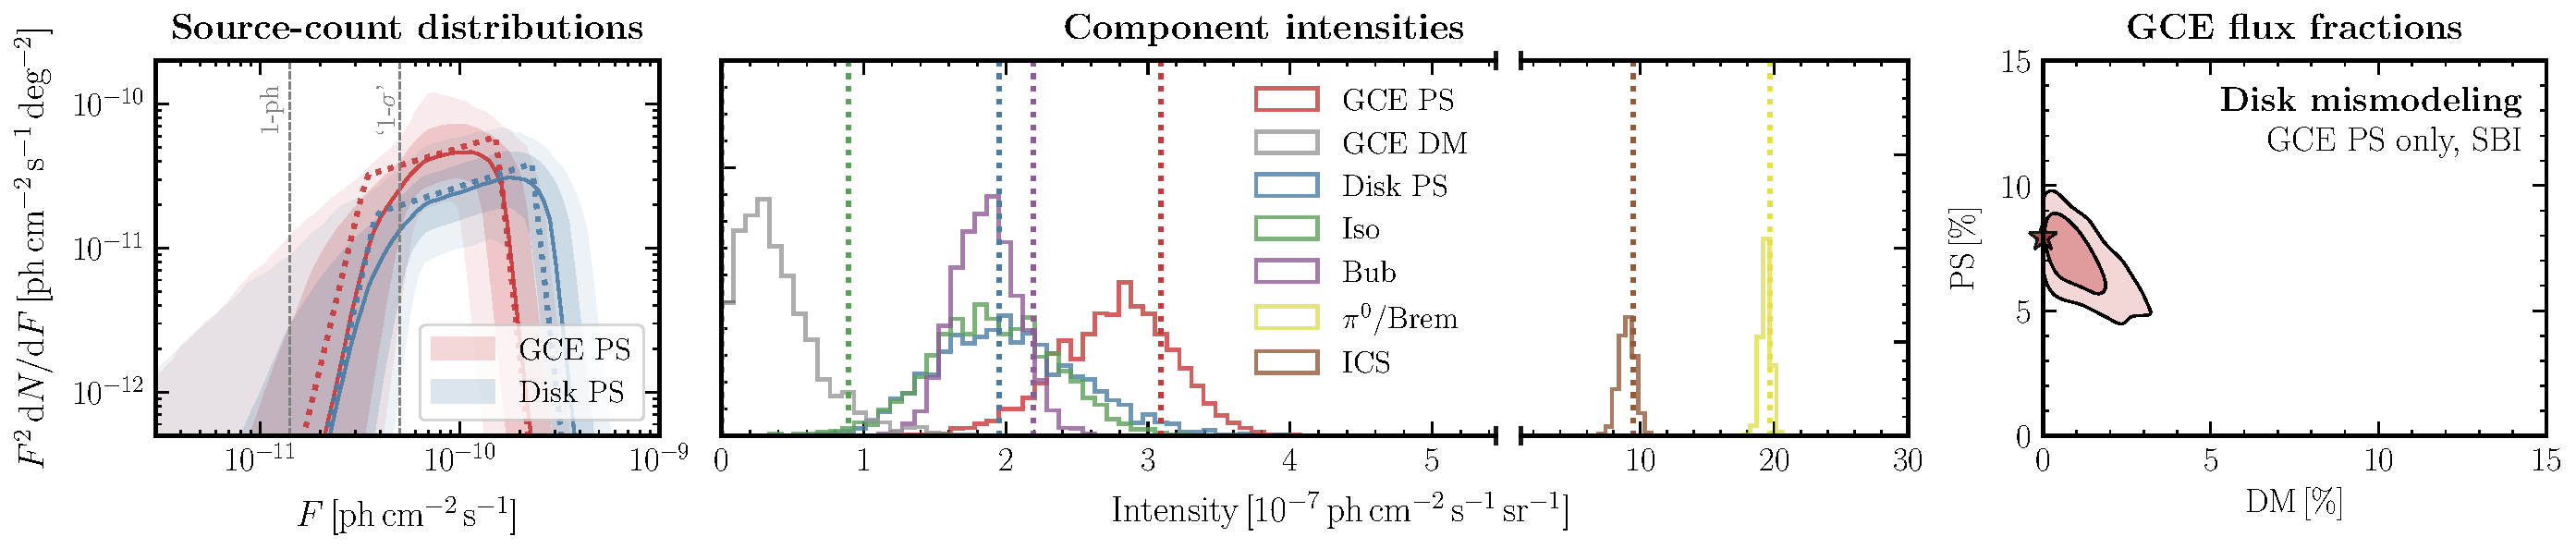
\includegraphics[width=0.95\textwidth]{plots/sim_sbi_thick_disk_mm_ps.pdf}
    \caption{Effect of mismodeling on a smooth GCE within our analysis framework. Each row shows aggregate posteriors collected over 10 simulated samples; row-wise from top to bottom: \emph{(i)} No mismodeling; simulated data is constructed with the same templates as those used in the forward model. \emph{(ii)} Mock data created with diffuse Model A, showing the effect of diffuse mismodeling. \emph{(iii)} Mock data where the diffuse template, described by Model O, is modulated by draws from a Gaussian process modeling large-scale mismodeling inferred from the real \Fermi data. \emph{(iv)} Mock data where the thick-disk template is used in lieu of the thin-disk template. \emph{(v)} Mock data where the GCE signal in the Northern hemisphere is twice as large as that in the Southern hemisphere. While some PS-like emission is inferred, it is consistent with zero in all cases, and evidence for a smooth GCE is robust.}
    \label{fig:sim_sbi_mismo}
    \end{figure*}
    %
    

\end{document}
